\documentclass[11pt,a4paper]{article}

\usepackage{graphicx}
\usepackage{color}
\usepackage{amsmath}
\usepackage{amssymb}
\usepackage{listings}
\usepackage{hyperref}

\lstset{language=c++}
\lstset{basicstyle=\tiny}
\lstset{backgroundcolor=\color{white}}
\lstset{frame=single}
\lstset{stringstyle=\ttfamily}
\lstset{keywordstyle=\color{red}\bfseries}
\lstset{commentstyle=\itshape\color{blue}}
\lstset{showspaces=false}
\lstset{showstringspaces=false}
\lstset{showtabs=false}
\lstset{breaklines}

\title{Computational Development of the 2D Ising Model}
\author{John Bower}
\date{May 5 2016}

\begin{document}
\maketitle

\begin{abstract}

In this project I investigate the 2D Ising Model.

\end{abstract}

\begin{itemize}
\item All source files and benchmark calculations can be found at \url{https://github.com/johnbower2012/CPMSU_work/tree/master/project4}.
\item A list of all code files can be found at the end of this document.
\end{itemize}

\section{Introduction}


Statistical Physics makes open those areas of interest involving quantities of particles far too large to be calculated normally, with numbers best measured in multiples of Avagadro's number, $6.022 x 10^23$. In this realm exact descriptions of specific states are replaced by bulk statements, mean values and systemwide properties. Through such methodologies, comprehensive descriptions of phase transitions in media, such as liquid to gas in water or liquid to superliquid in helium, are possible. An interesting and perhaps the classic example in this field is the Ising Model, a system wherein particles capable of only spin up or down are placed upon a grid in n-dimensions. By considering the interaction between neighboring spins, a description of the system's energy, magnetization, heat capacity, and magnetic susceptibility can be built, all from the simple description of its energy,
\begin{equation}
H = -J\sum\limits_{<ij>}s_is_j,
\end{equation}
where $J$ is the energy per spin pair, $<ij>$ describes a sum over only neighboring spins, and $s_i$ and $s_j$ are the respective spins of locations $i$ and $j$. From this statement of energy and 
an application of the Boltzmann distribution, where we say the probability of the system having an energy $E_i$ is
\begin{equation}
P(E_i) = \frac{e^{-E_i/T}}{\sum\limits^N_{i=1} e^{-E_i/T}} = \frac{e^{-E_i\beta}}{Z},
\end{equation}
where
\begin{equation}
\beta = \frac{1}{T}, \hspace{0.5 cm} Z = \sum\limits^N_{i=1} e^{-\beta E_i},
\end{equation}
we will investigate these bulk properties and search for a phase transition.

\section{Theory}

In this section we outline the mathematics of taylor expansions and the discretized notation in order to understand the approximations used in both the Verlet and Runge-Kutta methods.

\subsection{Taylor Expansion}

In principle, a taylor expansion uses an infinite series to exactly describe the behavior of a given function in terms of polynomial, that is given a function f(x) we may say
\begin{equation}
f(x+h) = \sum\limits_{i=0}^{\infty} \frac{h^i}{i!}f^{(i)}(x),
\end{equation}
where $f^{(i)}$ is the $i$th derivative of f(x) and $h$ is some small step in x. While the infinite series may be an exact description, in practice we are unable to sum to infinity and so must truncate at some step $n$,
\begin{align}
f(x+h) 	&\approx \sum\limits_{i=0}^{n} \frac{h^i}{i!}f^{(i)}(x) + O(h^{(n+1)})\\
		&= f(x) + hf^{(1)}(x) + \frac{h^2}{2}f^{(2)}(x) + \dots + \frac{h^n}{n!}f^{(n)}(x),
\end{align}
where we have noted that the error goes as $h^{(n+1)}$. 

Thus, given some function f(x) and its relation to its derivatives, we are able to approximate its evolution as we advance forward by some step size $h$, from $x \rightarrow x+h$.

\subsection{Discretization}

With the concept of taylor expansions settled, we turn our attention to discretizing the evolution of some function $f(x)$ across some range $x_{min} \rightarrow x_{max}$. Given some choice for the number of grid points, $n$, we define the step size, $h$ from above, as $h = \frac{x_{max} - x_{min}}{n}$, so that we may then say that our grid points are represented by the set which ranges from $x_0 = x_{min}, \dots, x_i = x_{min} + ih, \dots, x_n = x_{min} + nh = x_{max}$. Whereby we may define
\begin{equation}
f_{i+1} = f_i + hf^{(1)}_i + \frac{h^2}{2}f^{(2)}_i + \dots + \frac{h^n}{n!}f^{(n)}_i,
\end{equation}
so that given a set of initial conditions, $f^{(m)}(x_{min}) = a_m$, where $0\leq m \leq k$, we may calculate stepwise through to $f(x_{max})$.

Thus, we are ready to begin discussion of Verlet and Runge-Kutta. 

\section{Methodology}

In this section we discuss and implement the Verlet and Runge-Kutta algorithms themselves, building upon the work of the previous seection. My own code written for this task is included in my github repository, as seen at the beginning of the project, which includes method selections of RK4, Verlet, and Verlet with relativistic corrections coupled with optional output for the pure and complete evolution, output of once per earth year, and multiple choices for perihelion and aphelion outputs. The time of execution is written to screen for each method.

First however, we recognize that equation (1) may be rewritten from a second-order differential equation into two first-order differential equations by recognizing that
\begin{equation}
\frac{dx(t)}{dt} = v(t)
\end{equation}
so that
\begin{equation}
\frac{d^2x(t)}{dt^2} = \frac{dv(t)}{dt} = \frac{F(x(t),t)}{m}.
\end{equation}
Thus we may proceed by calculating both the body's position, x(t), and velocity, v(t), in small time steps $h$ given the total force, F(x(t),t), acting upon it. Note that we will be extending the discretized notation to both $x(t)$ and $t$, such that $x_i = x(t_i)$ and $t_i = t_{min} + ih$, whereby we may assume that $F_i = F(x_i, t_i) = F(x(t_i),t_i)$.


\subsection{Verlet Algorithm}

The Verlet algorithm involves an algebraic manipulation of taylor expansions. We begin by considering the expansions of x(t) and v(t) to second order. Thus, we have
\begin{align}
x(t+h) 	&= x(t) + h\frac{dx(t)}{dt} + \frac{h^2}{2}\frac{d^2x(t)}{dt^2} \\
		&= x(t) + hv(t) + \frac{h^2}{2}\frac{F(x(t),t)}{m}
\end{align}
and
\begin{align}
v(t+h) 	&= v(t) + h\frac{dv(t)}{dt} + \frac{h^2}{2}\frac{d^2v(t)}{dt^2} \\
		&= v(t) + h\frac{F(x(t),t)}{m} + \frac{h^2}{2}\frac{d^2v(t)}{dt^2}.
\end{align}
Here we notice that there is no obvious substition for $\frac{d^2v(t)}{dt^2}$, so we must once more consider an approximation. Expanding v(t+h) to first order,
\begin{equation}
v(t+h) 	= v(t) + h\frac{dv(t)}{dt},
\end{equation}
we see that by isolating $h\frac{dv(t)}{dt}$ and taking the derivative of each side, we arrive at
\begin{equation}
h\frac{d^2v(t)}{dt^2} = \frac{dv(t+h)}{dt} - \frac{dv(t)}{dt},
\end{equation}
or
\begin{align}
\frac{h^2}{2}\frac{d^2v(t)}{dt^2} &= \frac{h}{2}\bigg(\frac{dv(t+h)}{dt} - \frac{dv(t)}{dt}\bigg) \\
									&= \frac{h}{2}\bigg(\frac{F(x(t+h),t+h)}{m} - \frac{F(x(t),t)}{m}\bigg).
\end{align}
Whence we arrive at both x(t+h) and v(t+h)
\begin{align}
x(t+h) 	&= x(t) + h\frac{v(t)} + \frac{h^2}{2}\frac{F(x(t),t)}{m} \\
v(t+h)	&= v(t) + \frac{h}{2}\bigg(\frac{F(x(t+h),t+h)}{m} + \frac{F(x(t),t)}{m}\bigg).
\end{align}
Arriving in discretized fashion at our final form,
\begin{align}
x_{i+1} &= x_i + hv_i + \frac{h^2}{2}\frac{F_i}{m} \\
v_{i+1}	&= v_i + \frac{h}{2}\bigg(\frac{F_{i+1}}{m} + \frac{F_i}{m}\bigg),
\end{align}
we are now able to solve for both the final positions and velocities given only initial conditions and the relation of $\frac{d^2x(t)}{dt^2} = F(x(t), t)$.

\subsection{Runga-Kutta Algorithm (to fourth order)}

The Runge-Kutta algorithm follows from an implementation of the Fundamental Theorem of Calculus and Simpson's rule, namely
\begin{equation}
\int\limits_t^{t+h} f(t,y(t))dt = y(t+h) - y(t), \hspace{0.5 cm} where \frac{dy(t)}{dt} = f(t,y(t)),
\end{equation}
and
\begin{equation}
\int\limits_t^{t+h} f(t,y(t))dt = \frac{h}{6}\bigg(f(t,y(t)) + 4f\Big(t+\frac{h}{2},y\big(t+\frac{h}{2}\big)\Big)+f\Big(t+h,y\big(t+h\big)\Big)\bigg),
\end{equation}
respectively. By combining these two rules into discretized form, we see clearly that
\begin{align}
y_{i+1} &= y_i + \frac{h}{6}\Big(f\big(t_i,y_i\big) + 4f\big(t_{i+\frac{1}{2}},y_{i+\frac{1}{2}}\big)+f\big(t_{i+1},y_{i+1}\big)\Big) \\
		&= y_i + \frac{h}{6}\Big(f_i + 2f_{i+\frac{1}{2}} + 2f_{i+\frac{1}{2}} + f_{i+1}\Big)
\end{align}
where we have purposefully split the middle term into two equal halves and let $f_k = f(t_k,y_k)$. First, however, it is important to consider conceptionally what is happening. Here we are using a weighted average of slopes across the given $t \rightarrow t+h$ so as to better approximate the change from $y(t) \rightarrow y(t+h)$. With this in mind, we begin by rewriting our term as
\begin{equation}
y(t+h) = y(t) + \frac{h}{6}\big(k_1 + 2k_2 + 2k_3 + k_4\big),
\end{equation}
where we define the $k_1, \dots, k_4$ from the $f(t,y(t))$ in the following manner. Follow closely how each subsequent slope is used to determine the next.
\begin{align}
k_1 &= f_i \\
y_{i+\frac{1}{2}} &= y_i + \frac{h}{2}k_1 \\
k_2 &= f_{i+\frac{1}{2}} \\
y_{i+\frac{1}{2}} &= y_i + \frac{h}{2}k_2 \\
k_3 &= f_{i+\frac{1}{2}} \\
y_{i+1} = &= y_i + hk_3 \\
k_4 &= f_{i+1}
\end{align}
Hence we are finally able to calculate
\begin{equation}
y_{i+1} = y_i + \frac{h}{6}\big(k_1 + 2k_2 + 2k_3 + k_4\big),
\end{equation}
where all quantities on the right side are known. 
	While the above is the general method of implementing RK4, our method, however, is slightly more involved since we lack any general analytic form for the first deriative. Thus we must perform these calculations not only for $x(t)$, but also for $v(t,x(t))$. Thus we proceed as follows where we add an additional subscript on the $k$ values so as to keep the slopes for the position and velocity separate. Note also that in the following calculations $F_{i+\frac{1}{2}}$ refers to the new force at the new position $x_{i+\frac{1}{2}}$.
\begin{align}
k_{1v} & = F_i \\
k_{1x} &= v_i \\
x_{i+\frac{1}{2}} &= x_i + \frac{h}{2}k_{1x} \\
k_{2v} &= \frac{F_{i+\frac{1}{2}}}{m} \\
k_{2x} &= v_i + \frac{h}{2}k_{2v} \\
x_{i+\frac{1}{2}} &= x_i + \frac{h}{2}k_{2x} \\
k_{3v} &= \frac{F_{i+\frac{1}{2}}}{m} \\
k_{3x} &= v_i + \frac{h}{2}k_{3v} \\
x_{i+1} &= x_i + hk_{3x} \\
k_{4v} &= \frac{F_{i+1}}{m} \\
k_{4x} &= v_i + hk_{4v} \\
\end{align}
Whence we are able to calculate both $x_{i+1}$ and $v_{i+1}$ as
\begin{align}
x_{i+1} &= x_i + \frac{h}{6}\big(k_{1x} + 2k_{2x} + 2k_{3x} + k_{4x}\big) \\
v_{i+1} &= v_i + \frac{h}{6}\big(k_{1v} + 2k_{2v} + 2k_{3v} + k_{4v}\big).
\end{align}
Whence we are able to calculate the evolution of our system given initial conditions and with some specified total force. 

\subsection{Expansion to Three Dimensions, n-bodies}

In our example problem, we model first a two body system in two dimensions, then an n-body system in three dimensions, both plus time. Note that this only adds extra subscripts to our positions and velocities, such that we have three independent axes which follow the same evolution. The only mixing comes from the force which in our case relies on the magnitude of the relative position vectors. Thus we would proceed as above in both algorithms, except that we must first calculate the new position along each axis, $x_{i+1}, y_{i+1}, z_{i+1}$, in order to calculate the magnitude of the position vector, $r_{i+1}$. With this, we are then able to calculate the new force vector, $F_{i+1}$, and so calculate the velocities. 

When considering the case of simultaneously mobile n-bodies, the method proceeds exactly as above, excepting that once all new positions are calculated for the first body, they must be calculated for each other body before the net forces may be calculated. Note that the net force on a given body $i$ will simply be the superposition of the other bodies acting upon it.

Thus, with three dimensions (plus time) and n-bodies, the formula is simply to calculate the new position for each body, the new forces given the new positions, and then the new velocities given the new forces and positions. 

\section{Results}

Here we begin by observing the stability and speed of each algorithm using the case of circular motion of the earth around the sun. We observe the radius of the earth after a number of revolutions around the sun given different numbers of gri	d points. The code is written in project3.cpp, which links to project3-library.h. If compiled from command line in the same folder and no additions are required to "g++ -o project3.x project3.cpp." Unit tests for conservation of energy and momentum are included in project3-unittest.cpp which links to project3-library-unittest.h. In Figure (1) we see a comparison of the times for each metholodogy over a period of five years. In Figure (2) we see the case of earth-sun circular motion. In Figures (3), (4), and (5) we see a comparison of various initial speeds for earth until it escapes orbit. In Figures (6), (7), and (8) we see the effect of the addition of Jupiter, with its regular mass, ten times its mass, and one thousand times its mass, on earth's orbit around the sun. In Figures (9) and (10) we see the evolution of the full solar system over 250 years, in (11) and (12) of the interior planets given a full system over 50 years. 

\begin{figure}
\centering
\begin{tabular}{| l | l | l | l | l | l | l |}
\hline
n  	 & RK4 & RK4 time [s] & Verlet & Verlet time [s] & V. Rel. Cor & V.RC time[s]  \\ \hline
100   &  0.77813979  &  0.000188   &   1.004426   & 7.7e-5    & 1.0010571 & 6.3e-5 \\ \hline
200   &  0.98847564  &  0.000354   &  1.0001543   & 0.000105  & 1.0000138 & 9.2e-5 \\ \hline
500   &  0.9993386 	 &  0.00061    &  1.0000026   & 0.000313  & 1.0000001 & 0.000244 \\ \hline
1000   &  0.99991847 &  0.001717   &  1.0000001	  & 0.00052   & 1		  & 0.000493 \\ \hline
2000   &  0.99998984 &  0.002993   &   1	 	  & 0.00102   & 1		  & 0.000875 \\ \hline
5000   &  0.99999935 &  0.006268   &   1		  & 0.001993  & 1		  & 0.002277 \\ \hline
10000  &  0.99999992 &  0.014253   &   1		  & 0.004282  & 1		  & 0.005601 \\ \hline
\end{tabular}
\caption{A table for the evolution of the circular motion earth-sun system after a period of five years. The exact answer should be a radius of one AU. The number of grid points is given under $n$, with the final radius and computation time given for the RK4, Verlet, and Verlet with relativistic correction provided in the corresponding row. It seems clear that at high enough values of n, the Verlet algorithm is approximately three times faster than the RK4, with the VRC lying between them. This implementation for the RK4 algorithm approaches the eact solution from the bottom, whereas the Verlet approaches from above. An examination of the data over the course of the five years reveals that the radius and velocity remain constant, with their direction perpendicular, so the potential and kinetic energies, as well as the angular momentum, remain constant.}
\end{figure}
\begin{figure}
\centering
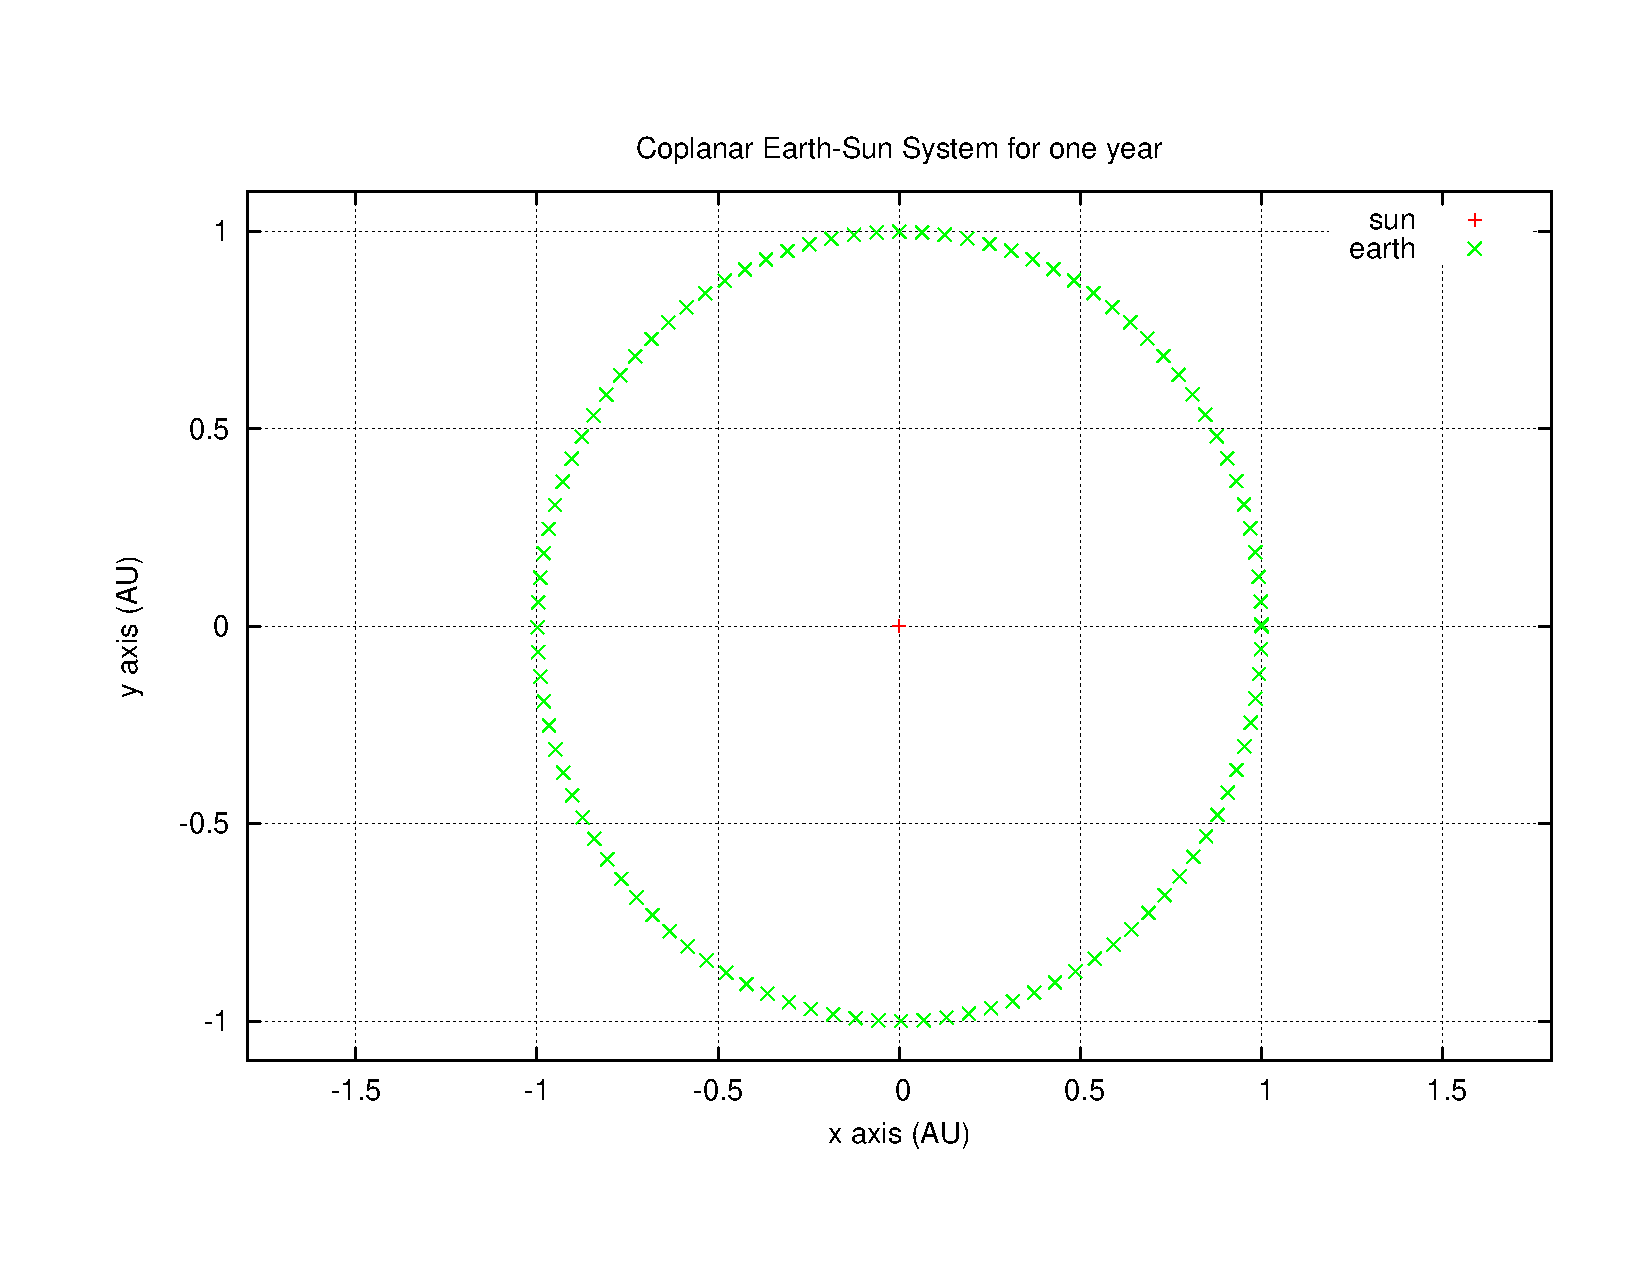
\includegraphics[width=1.0\textwidth]{coplanar_earthsun.pdf}
\caption{Here we see the coplanar earth-sun system with no evolution for the sun considered. The earth remains in a near perfect circular orbit given a starting speed of 2$\pi$ AU/yr and a radius of one AU.}
\end{figure}
\begin{figure}
\centering
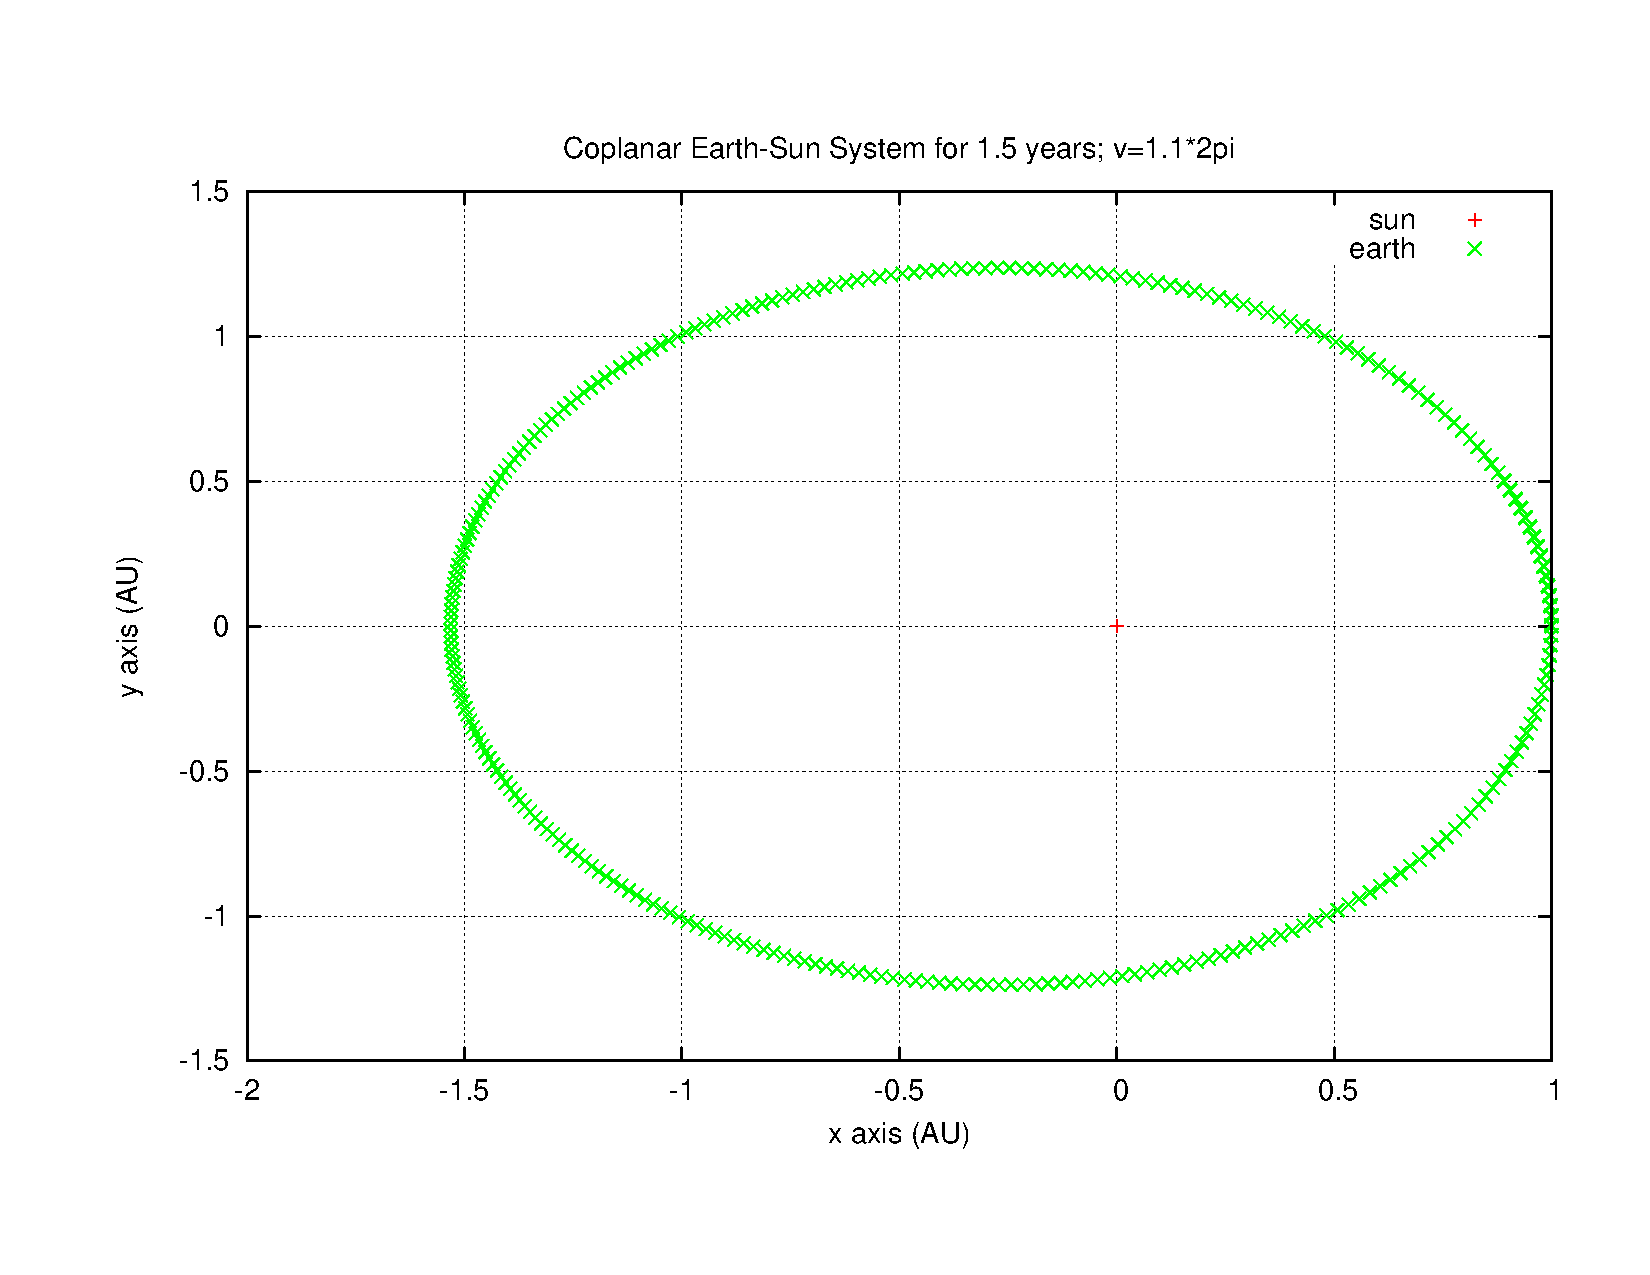
\includegraphics[width=1.0\textwidth]{coplanar_earthsun_v11.pdf}
\caption{Here we see the coplanar earth-sun system with no evolution for the sun considered. The earth has been given an initial speed of 2.2$\pi$. We observe that the orbit has become noticeable elliptical, with an aphelion of over 1.5 AU and a period of approximately 1.5 years.}
\end{figure}
\begin{figure}
\centering
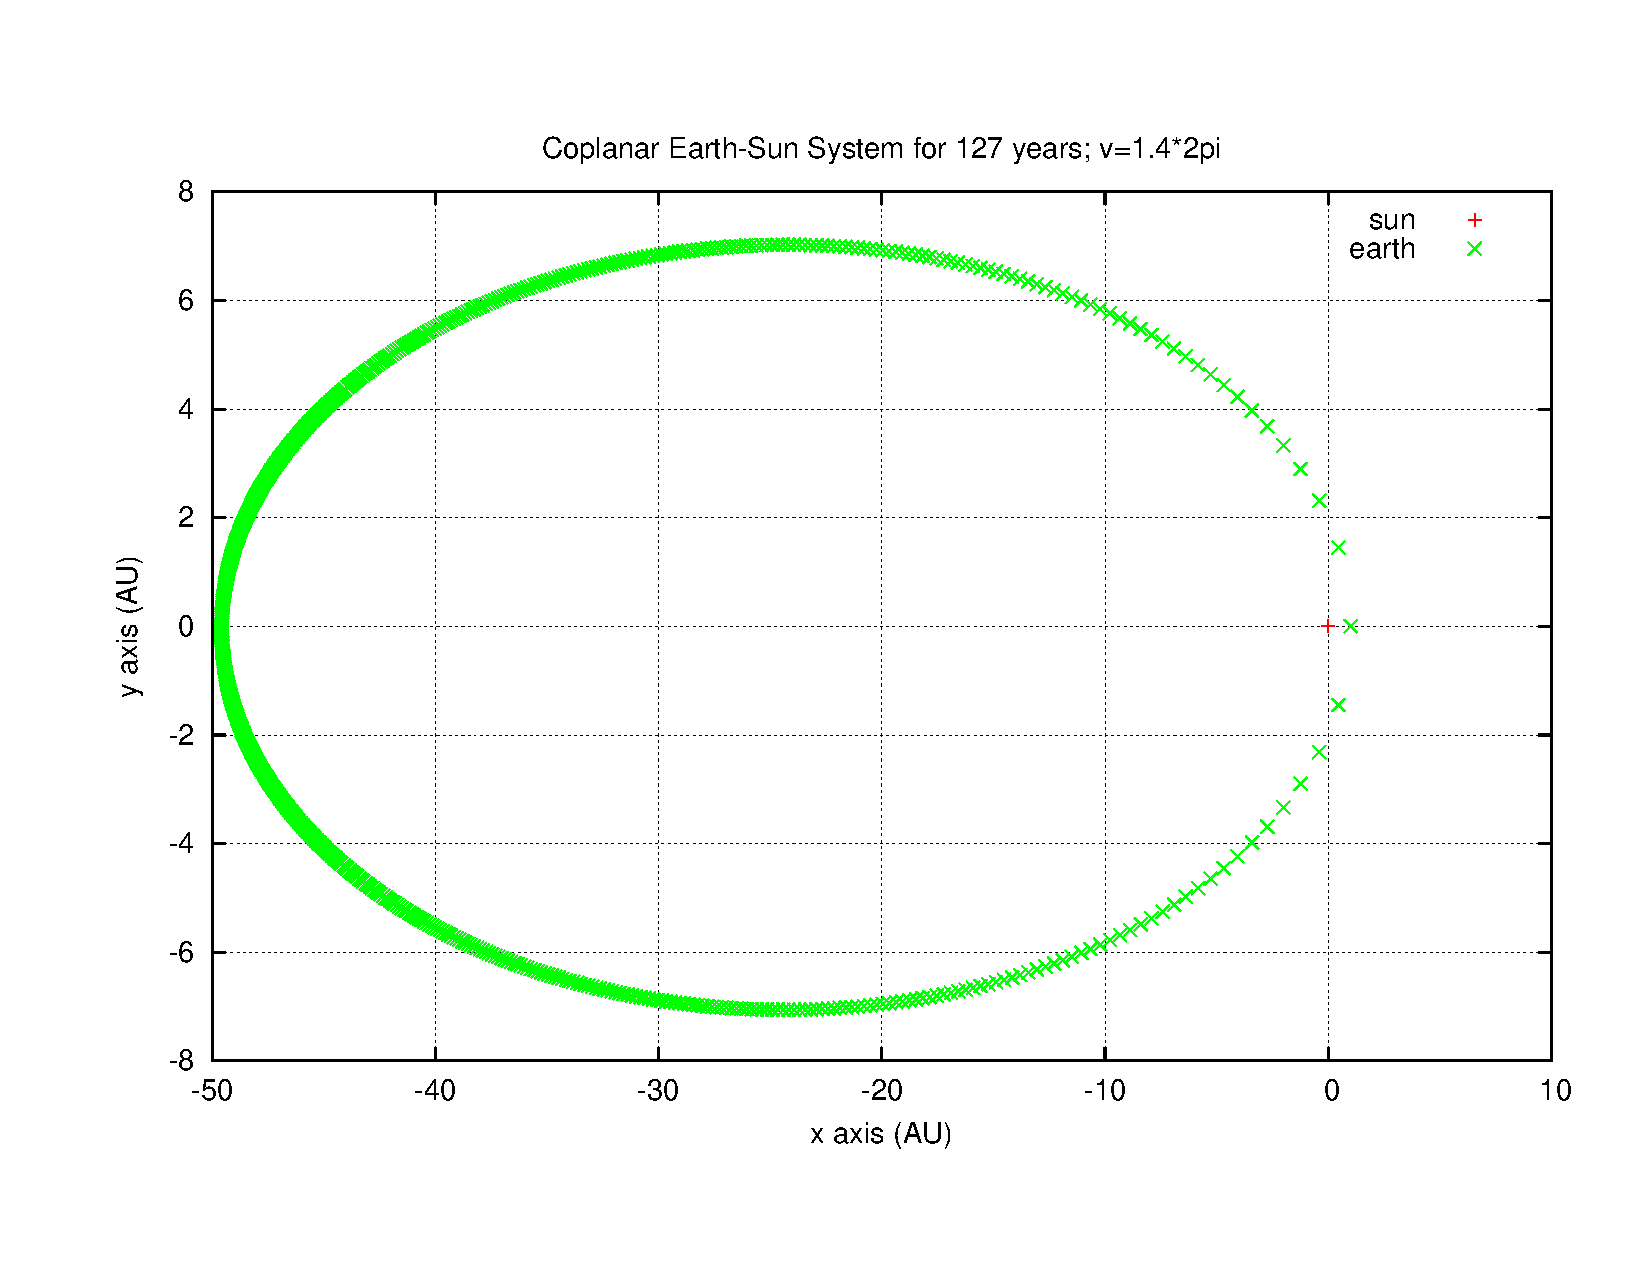
\includegraphics[width=1.0\textwidth]{coplanar_earthsun_v14.pdf}
\caption{Here we see the coplanar earth-sun system with no evolution for the sun considered. The earth has been given an initial speed of 2.8$\pi$. The earth's orbit has become widely elliptical, with an aphelion of over fifty AU and an orbital period of approximately 127 years. It has nearly reached escape velocity.}
\end{figure}
\begin{figure}
\centering
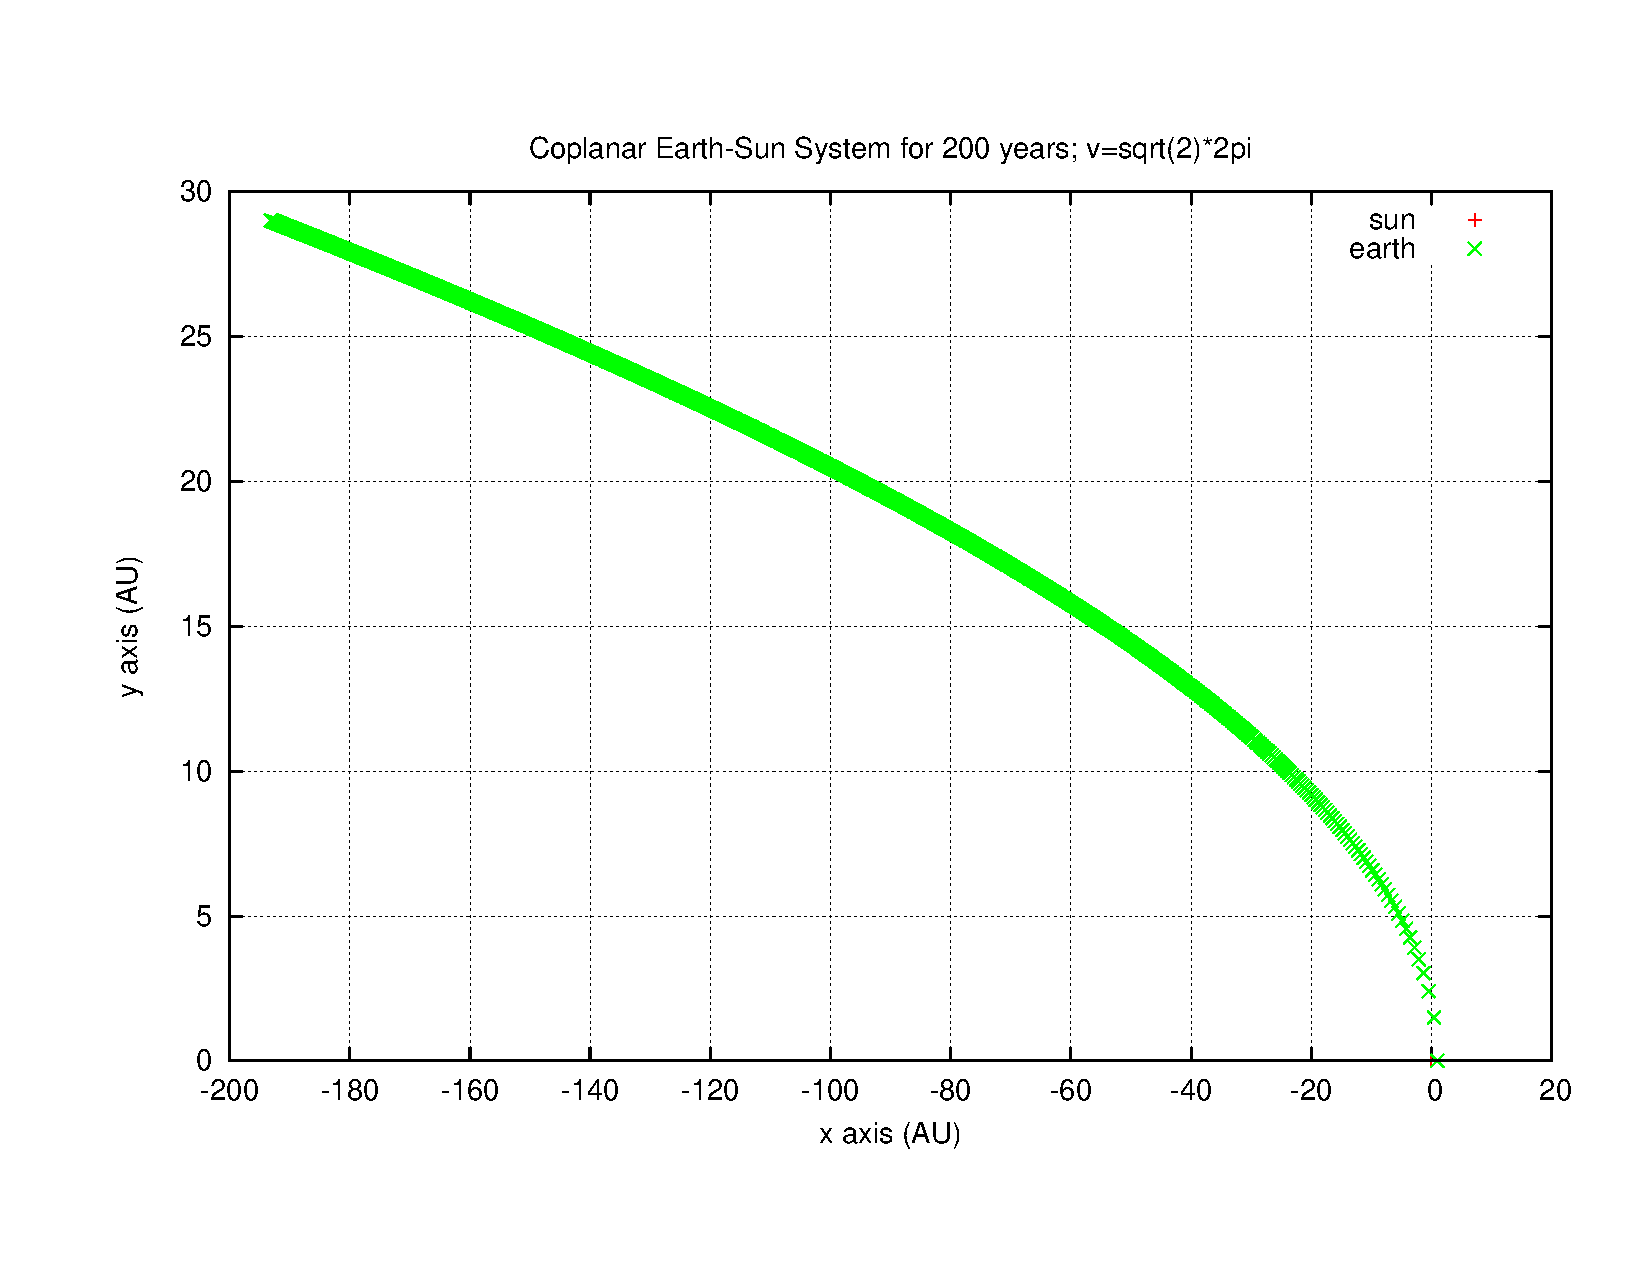
\includegraphics[width=1.0\textwidth]{coplanar_earthsun_vsqrt2.pdf}
\caption{Here we see the coplanar earth-sun system with no evolution for the sun considered. The earth has been given an initial speed of 2$\sqrt{2}\pi$, which equals the calculated escape velocity. Clearly, the earth has formed a hyperbolic curve and will not be returning to the sun. The calculation shown was an evolution of 200 years, and higher time frames were conducted as verification.}
\end{figure}
\begin{figure}
\centering
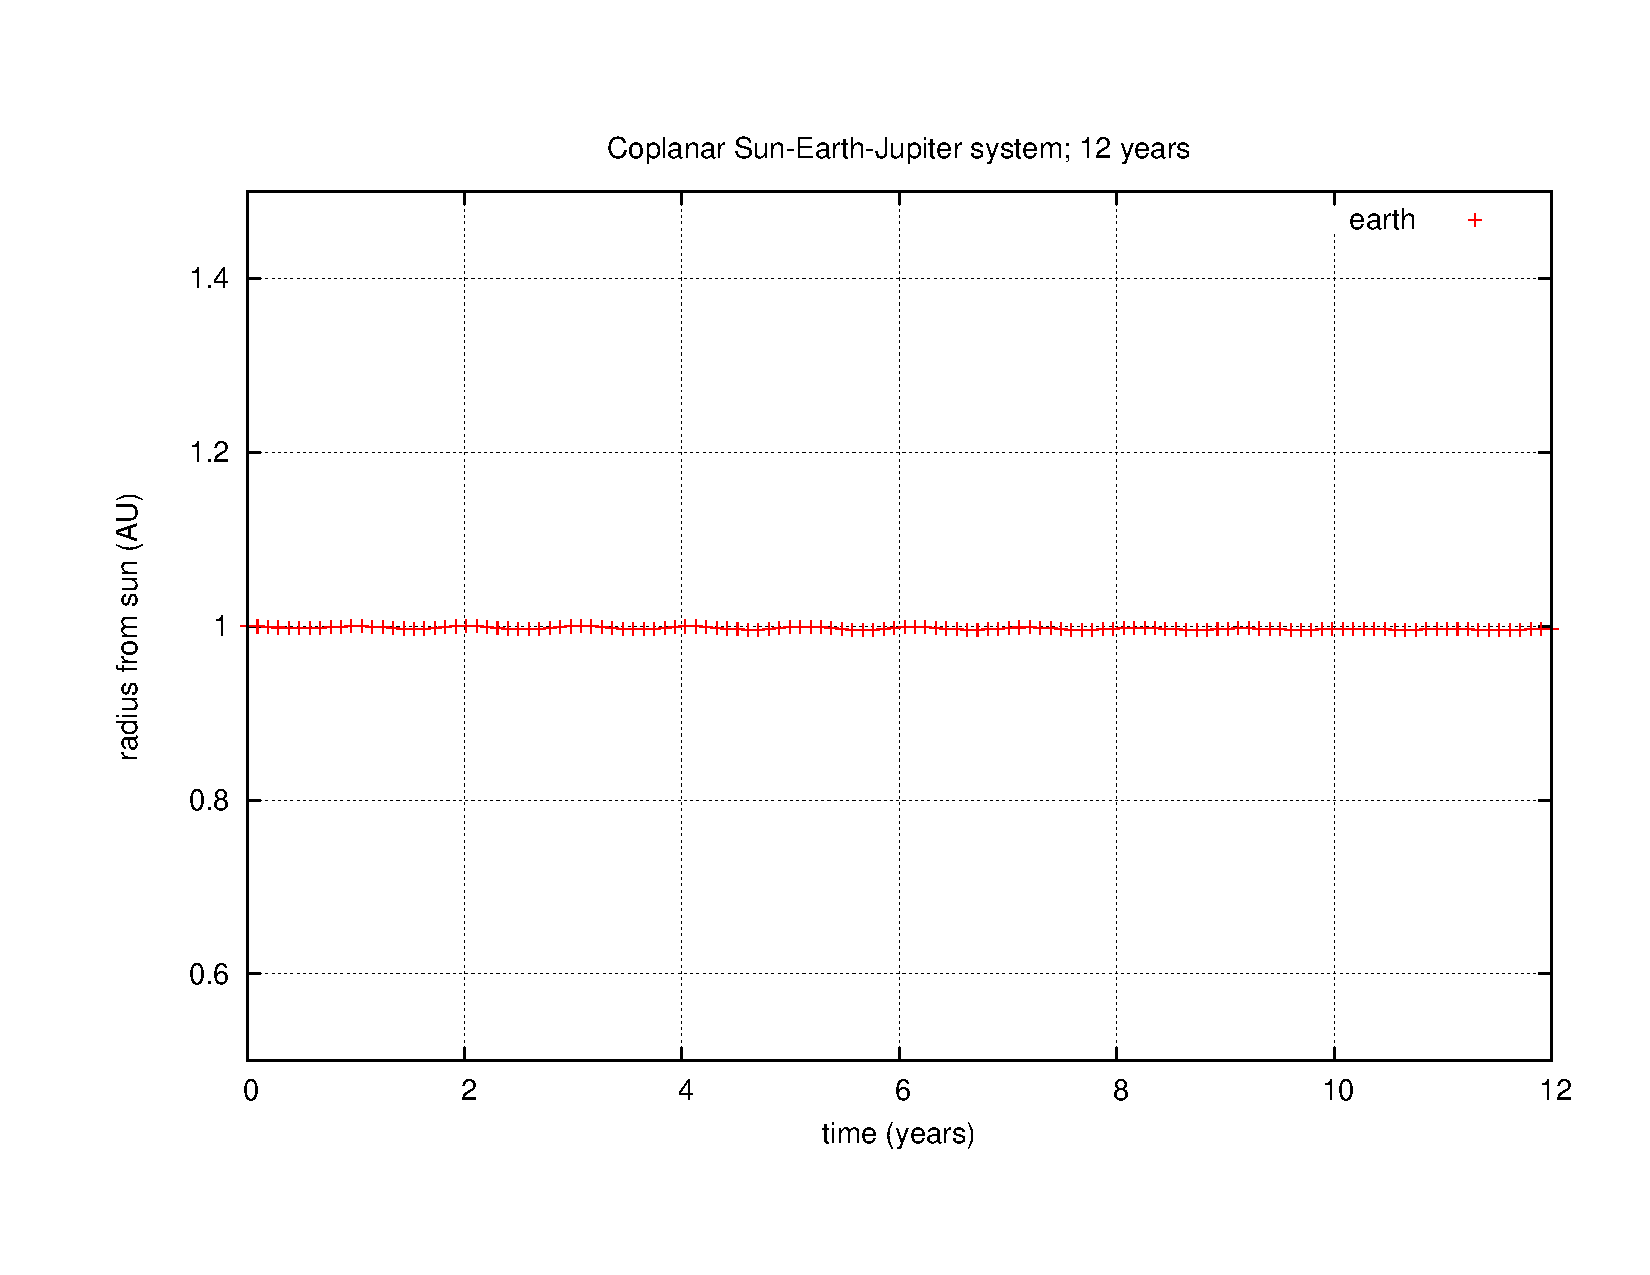
\includegraphics[width=1.0\textwidth]{coplanar_sej1_radius.pdf}
\caption{Here we see effect of the coplanar sun-earth-jupiter system on the earth's orbit with no evolution for the sun considered. The planets have each been given their respective mean orbital radius and velocity as initial conditions. We see that while Jupiter provides only small perturbations, they are clearly visible.}
\end{figure}
\begin{figure}
\centering
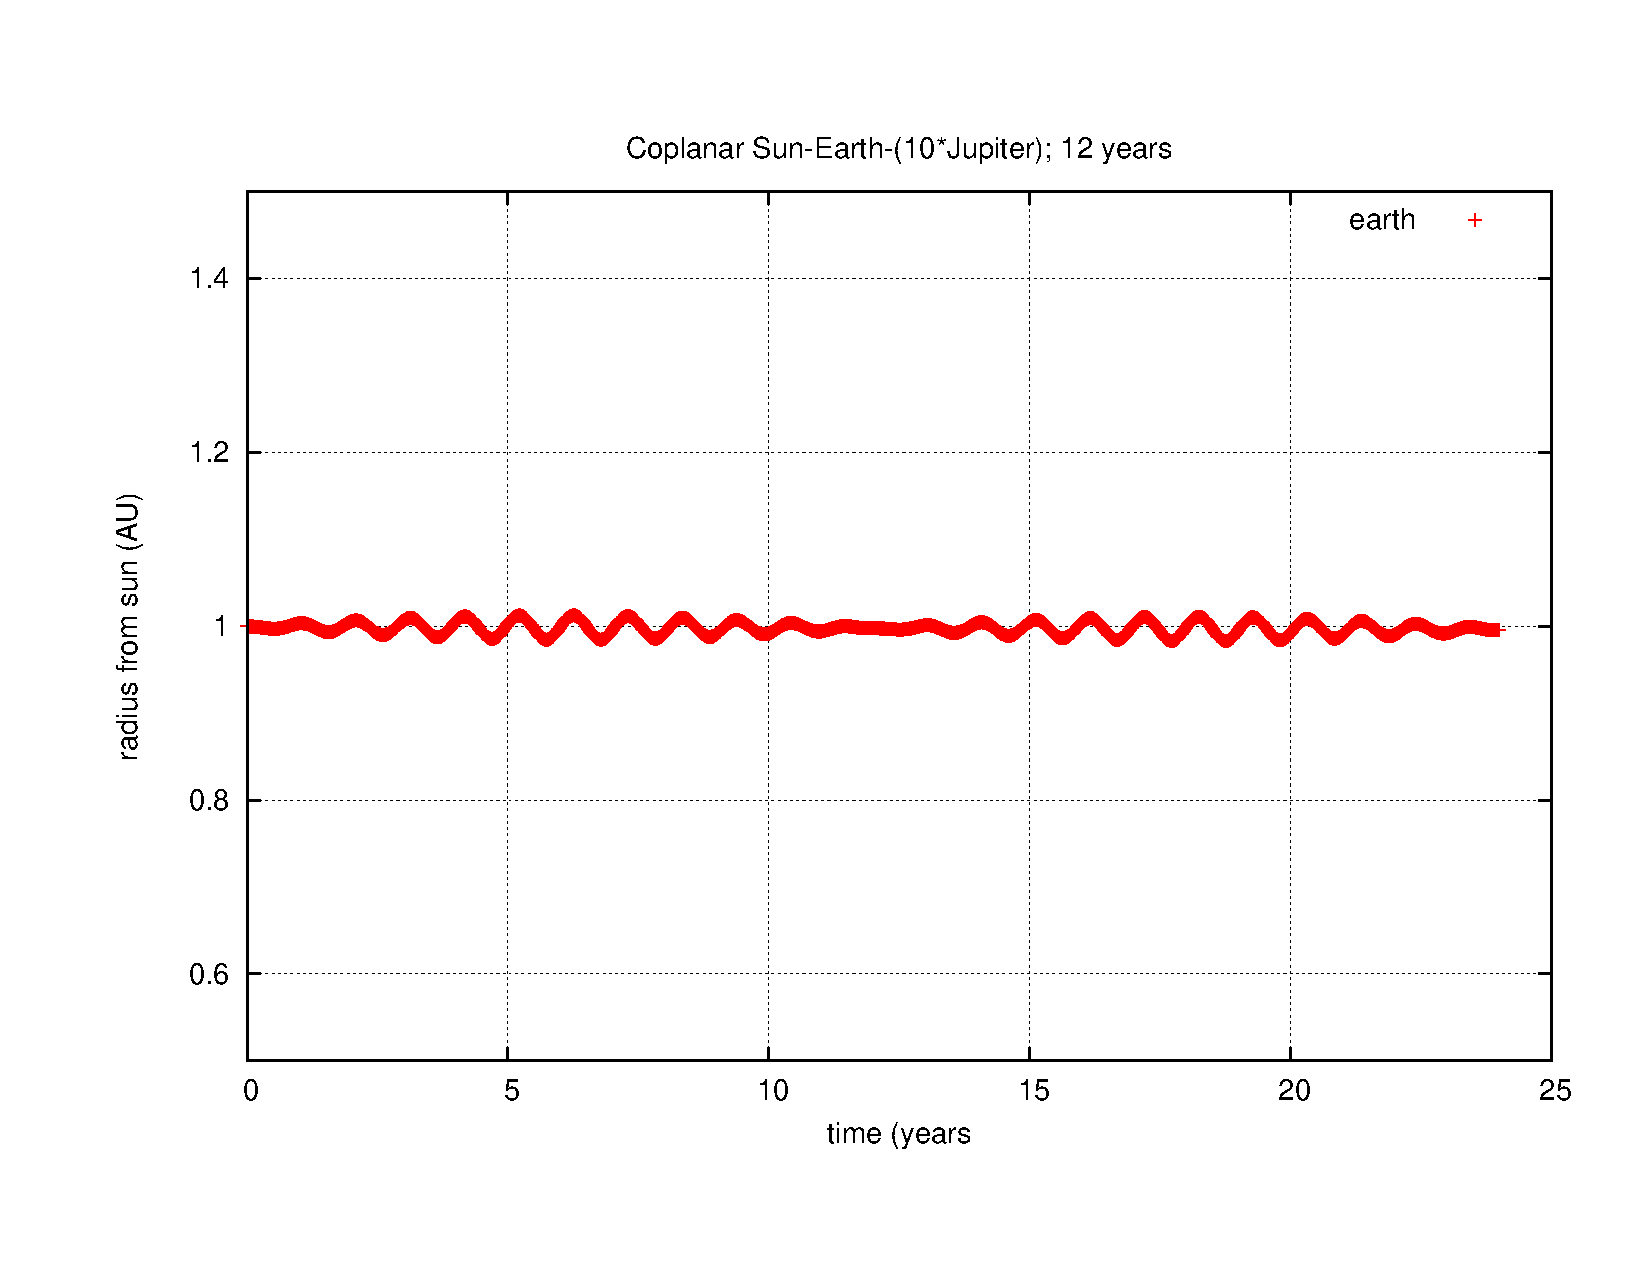
\includegraphics[width=1.0\textwidth]{coplanar_sej10_radius.pdf}
\caption{Here we see effect of the coplanar sun-earth-jupiter system on the earth's orbit with Jupiter's mass increased tenfold. The planets have each been given their respective mean orbital radius and velocity as initial conditions. We see that an increase in Jupiter's mass provides larger perturbations, but it appears to be periodic and results in a stable orbit for the earth.}
\end{figure}
\begin{figure}
\centering
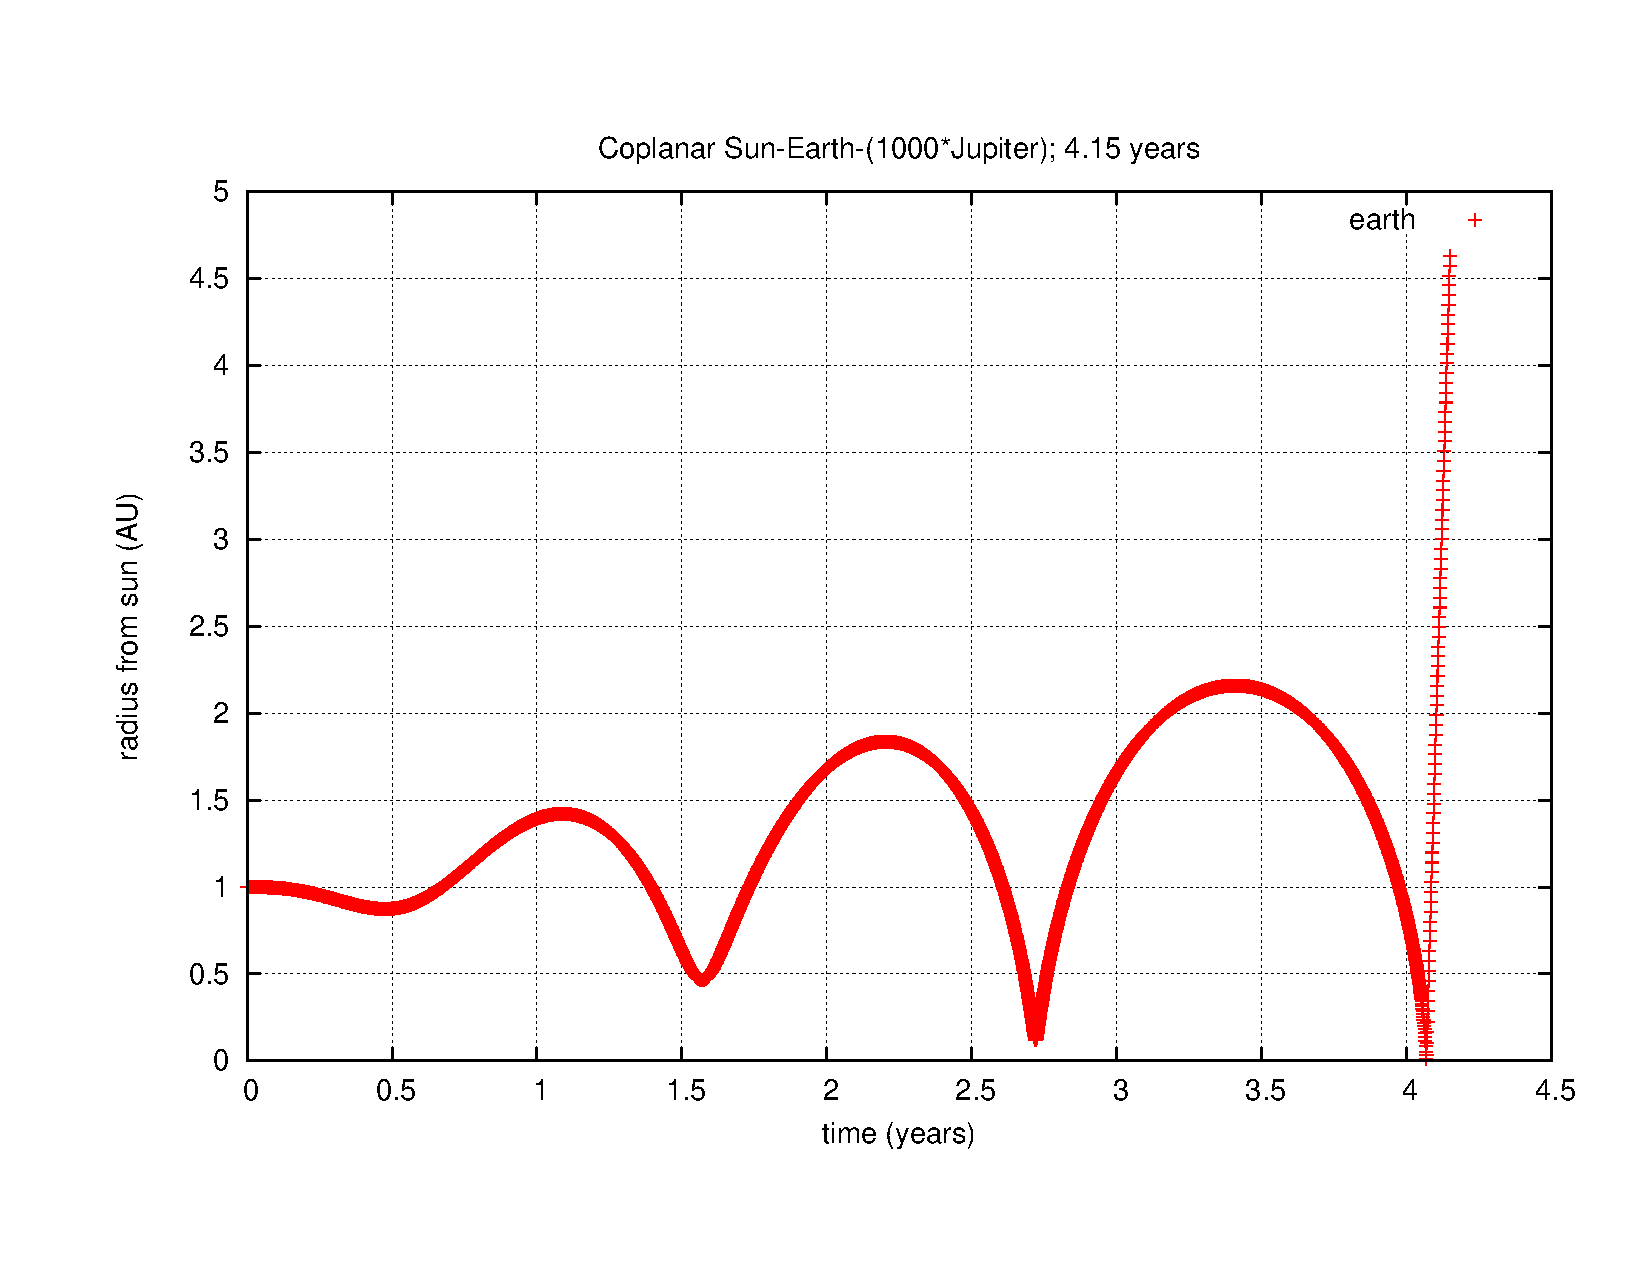
\includegraphics[width=1.0\textwidth]{coplanar_sej1000_radius.pdf}
\caption{Here we see effect of the coplanar sun-earth-jupiter system on the earth's orbit with Jupiter's mass increased thousandfold. The planets have each been given their respective mean orbital radius and velocity as initial conditions. We see that such an increase to Jupiter's mass creates an orbit which, after merely four years, sling shots earth from the solar system. The earth approaches the sun more and more closely during each pass and finally is launched from the solar system. Evolutions for much larger time frames were considered, but this is the best for viewing the initial gain of velocity leading to the expulsion of earth.}
\end{figure}
\begin{figure}
\centering
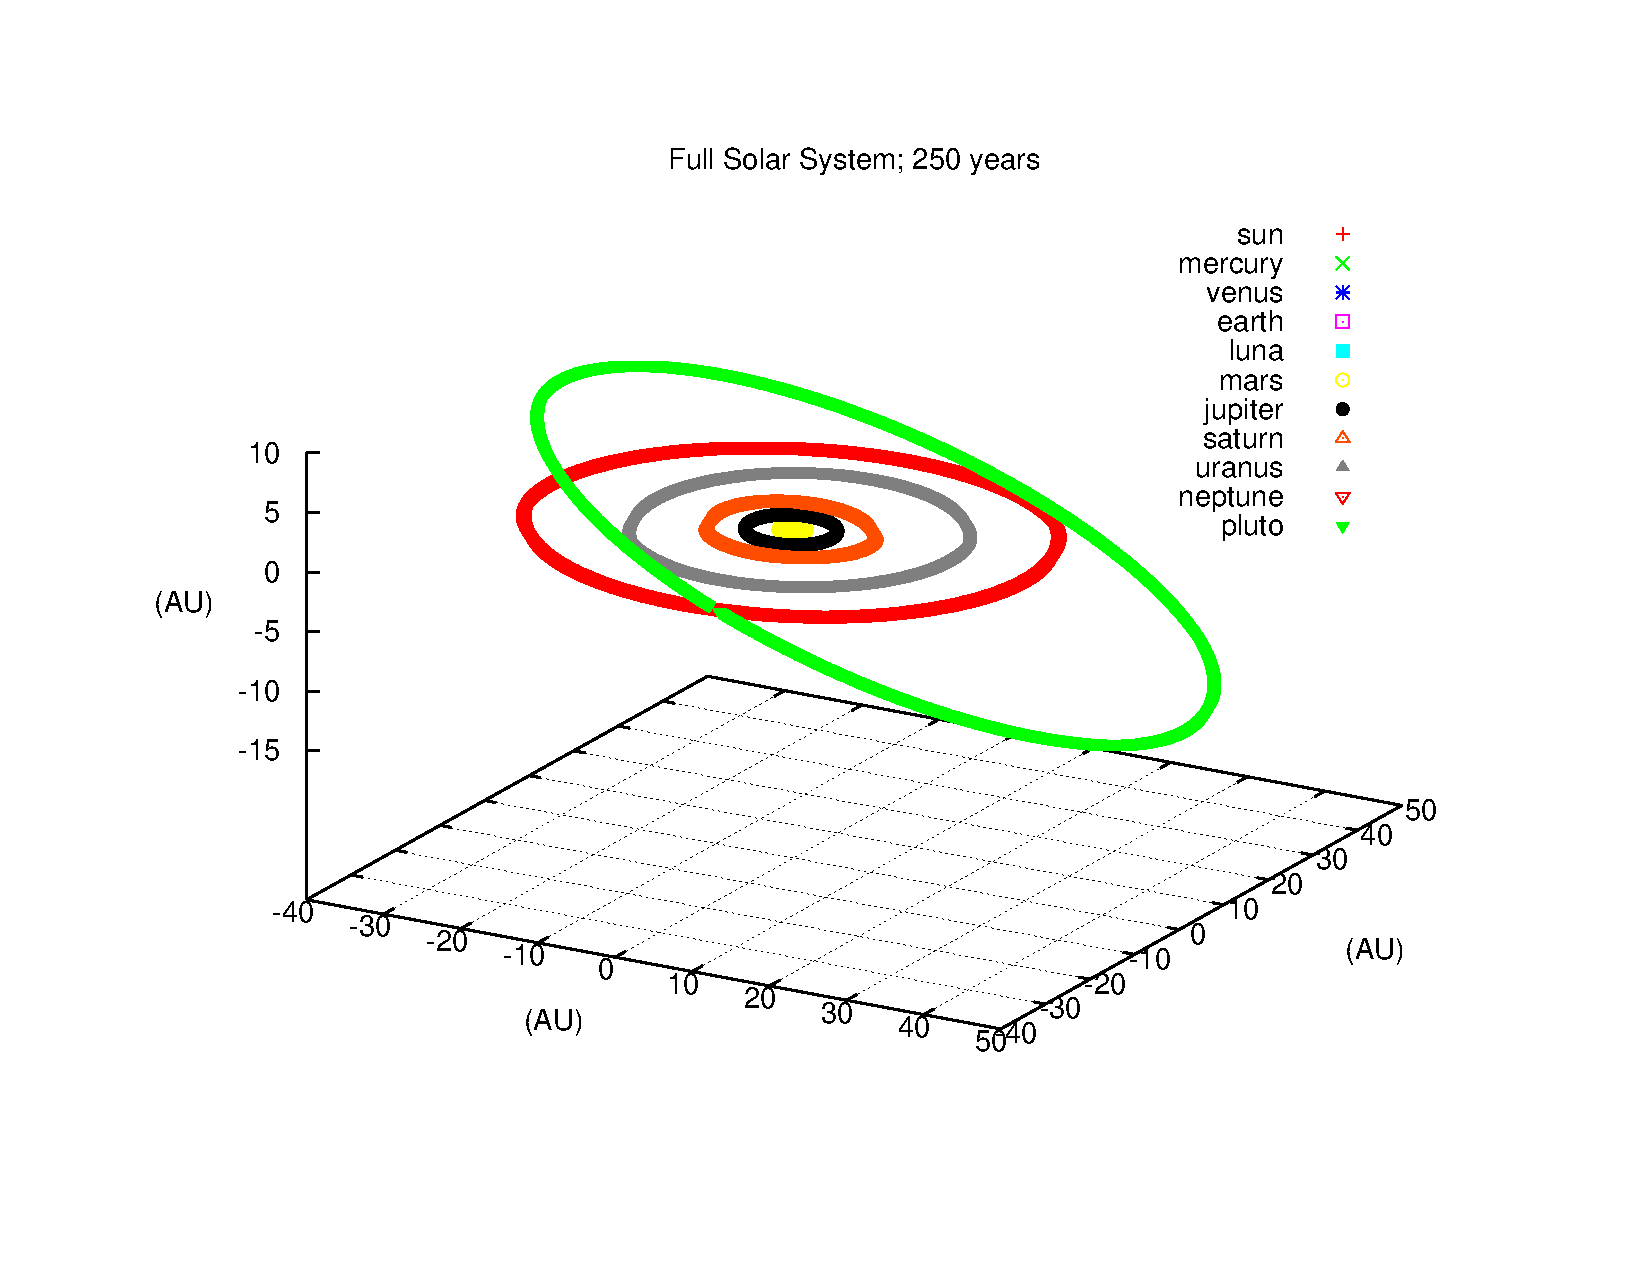
\includegraphics[width=1.0\textwidth]{fullss_250years.pdf}
\caption{Here we see the full solar system with initial conditions given from data on the Jet Propulsion Laboraty's website of March 18, 2016. The evolution is allowed to develop for 250 years see the near full revolution of pluto, the body with the longest orbital period and highest eccentricity. From this scale, we cannot see the inner panets, but we see they must have stable orbits since they have not left the solar system. We see that for a short time pluto is closer to the sun than neptune. The data file shows this much more clearly than the graph.}
\end{figure}
\begin{figure}
\centering
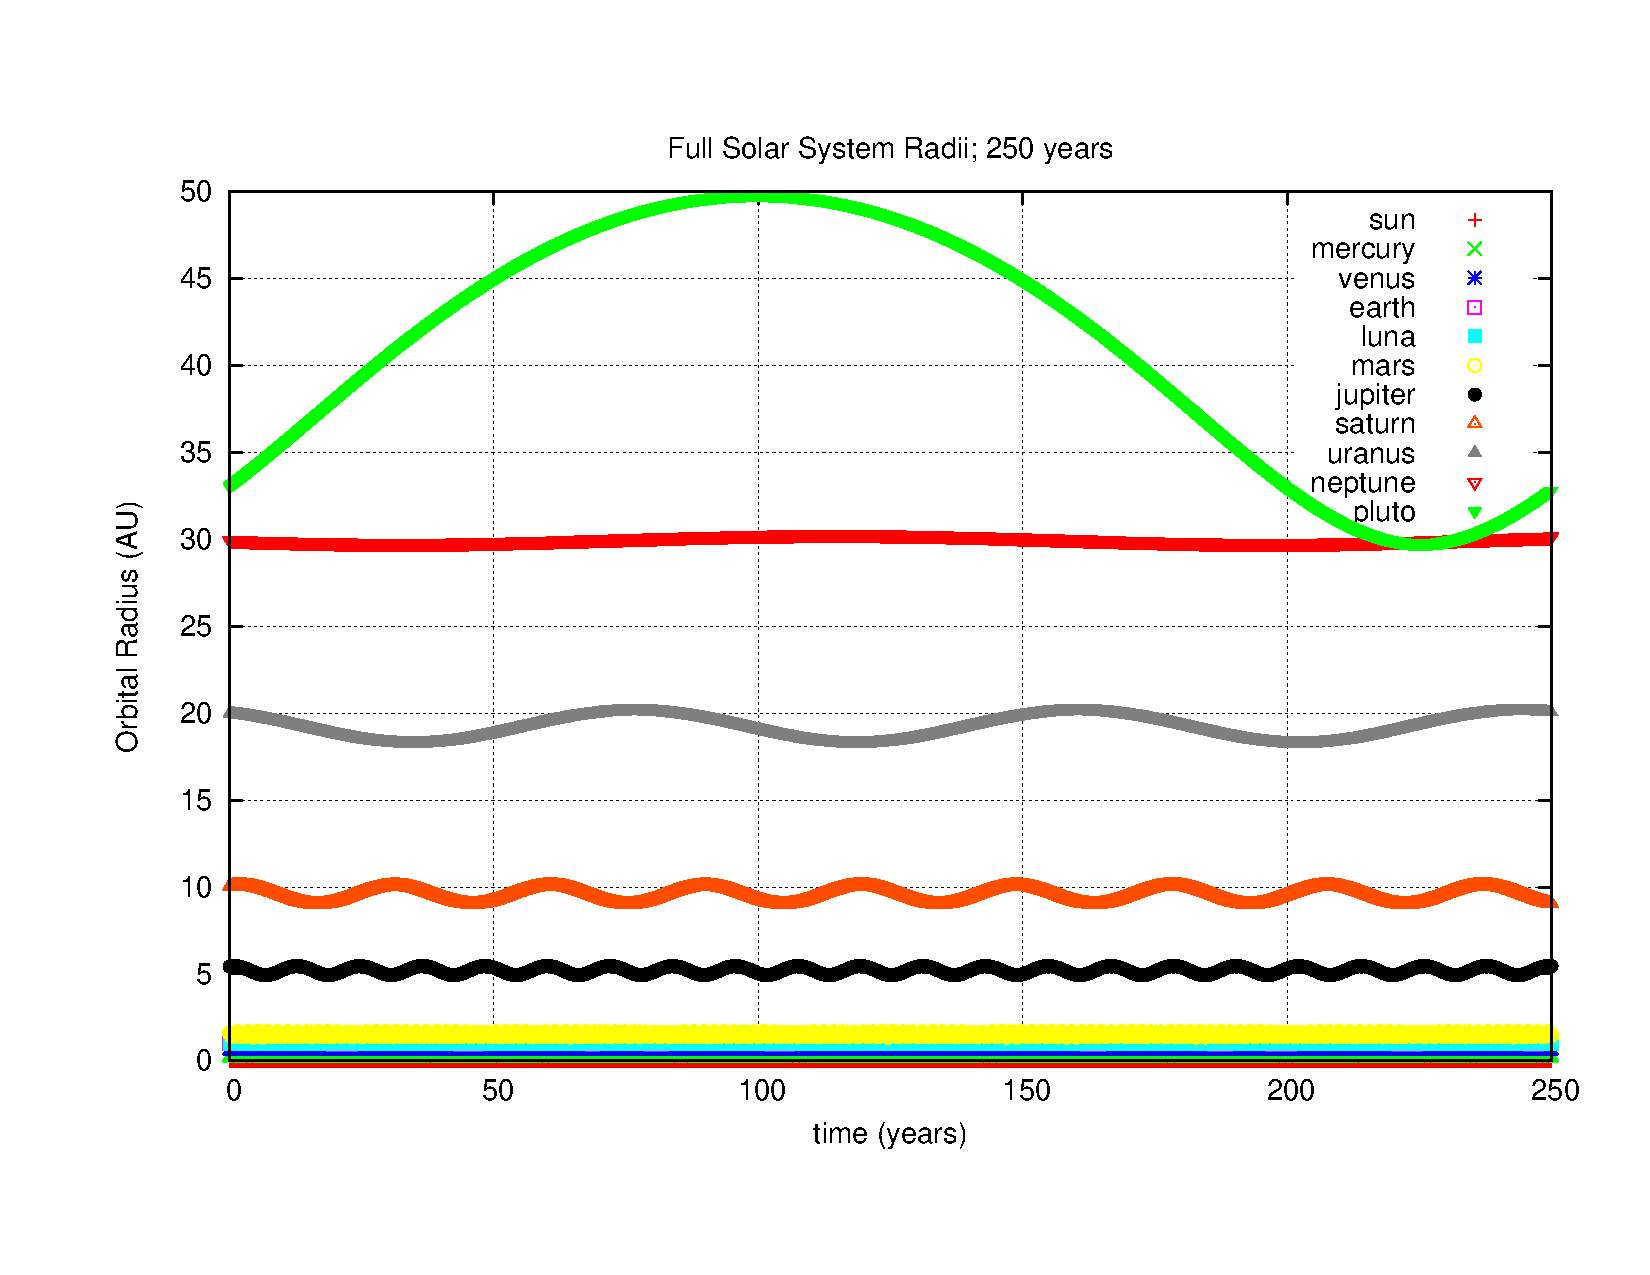
\includegraphics[width=1.0\textwidth]{fullss_radii_250years.pdf}
\caption{Here we see the orbital radii over the full 250 year evolution of the solar system from the previous figure. We see that the planets with the highest eccentricity have the most oscillatory orbits. Pluto clearly comes closer to the sun near the end of the 250 years, so once during its orbit. Also we observe that the approximate period can be determined from graph by measuring the distance from one maximum to the next, or one minimum to the next.}
\end{figure}
\begin{figure}
\centering
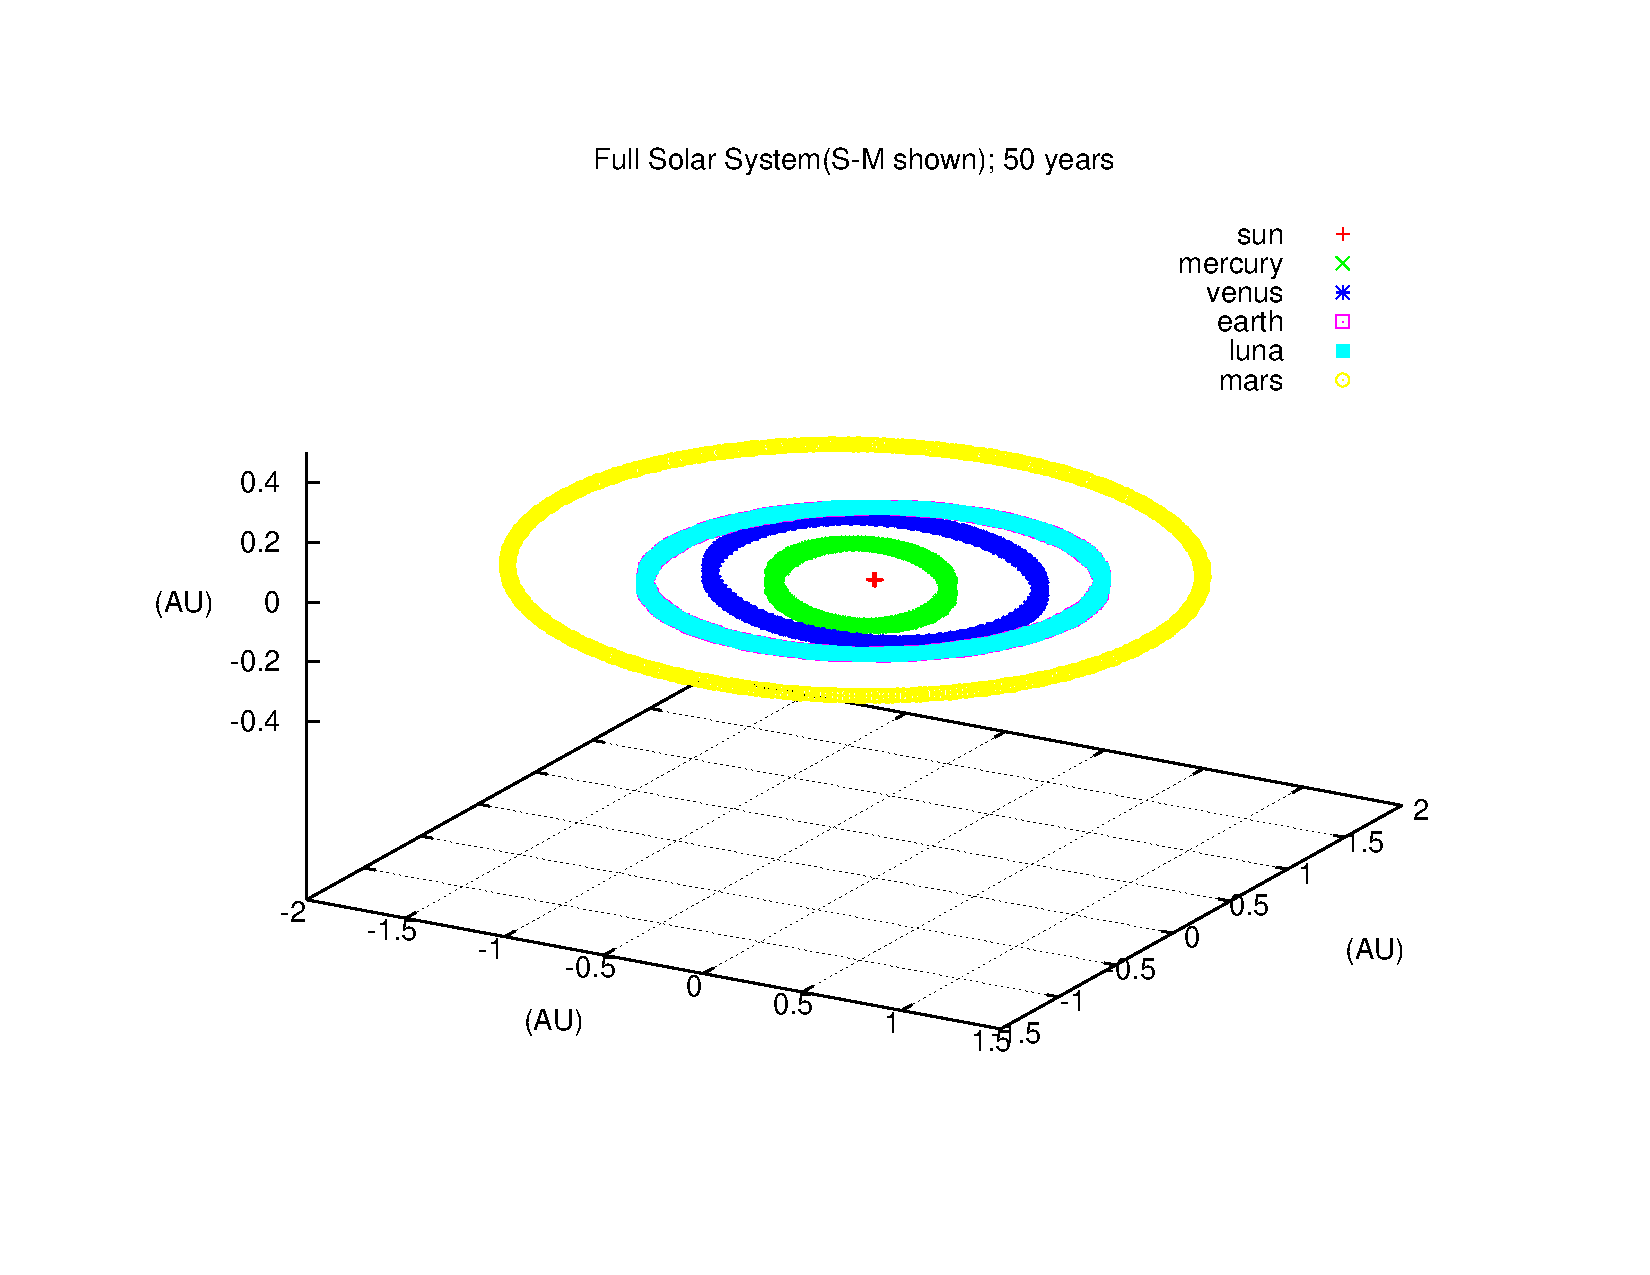
\includegraphics[width=1.0\textwidth]{fullss_s-m_50years.pdf}
\caption{Here we see the evolution of the solar system over 50 years, where all bodies were used for the calculation but only the inner have been plotted for clarity. Note that most inner planets have fairly circular orbits, with mercury being the most elliptical. Luna is the earth's moon, very clearly overlapping the orbit of the earth at this scale.}
\end{figure}
\begin{figure}
\centering
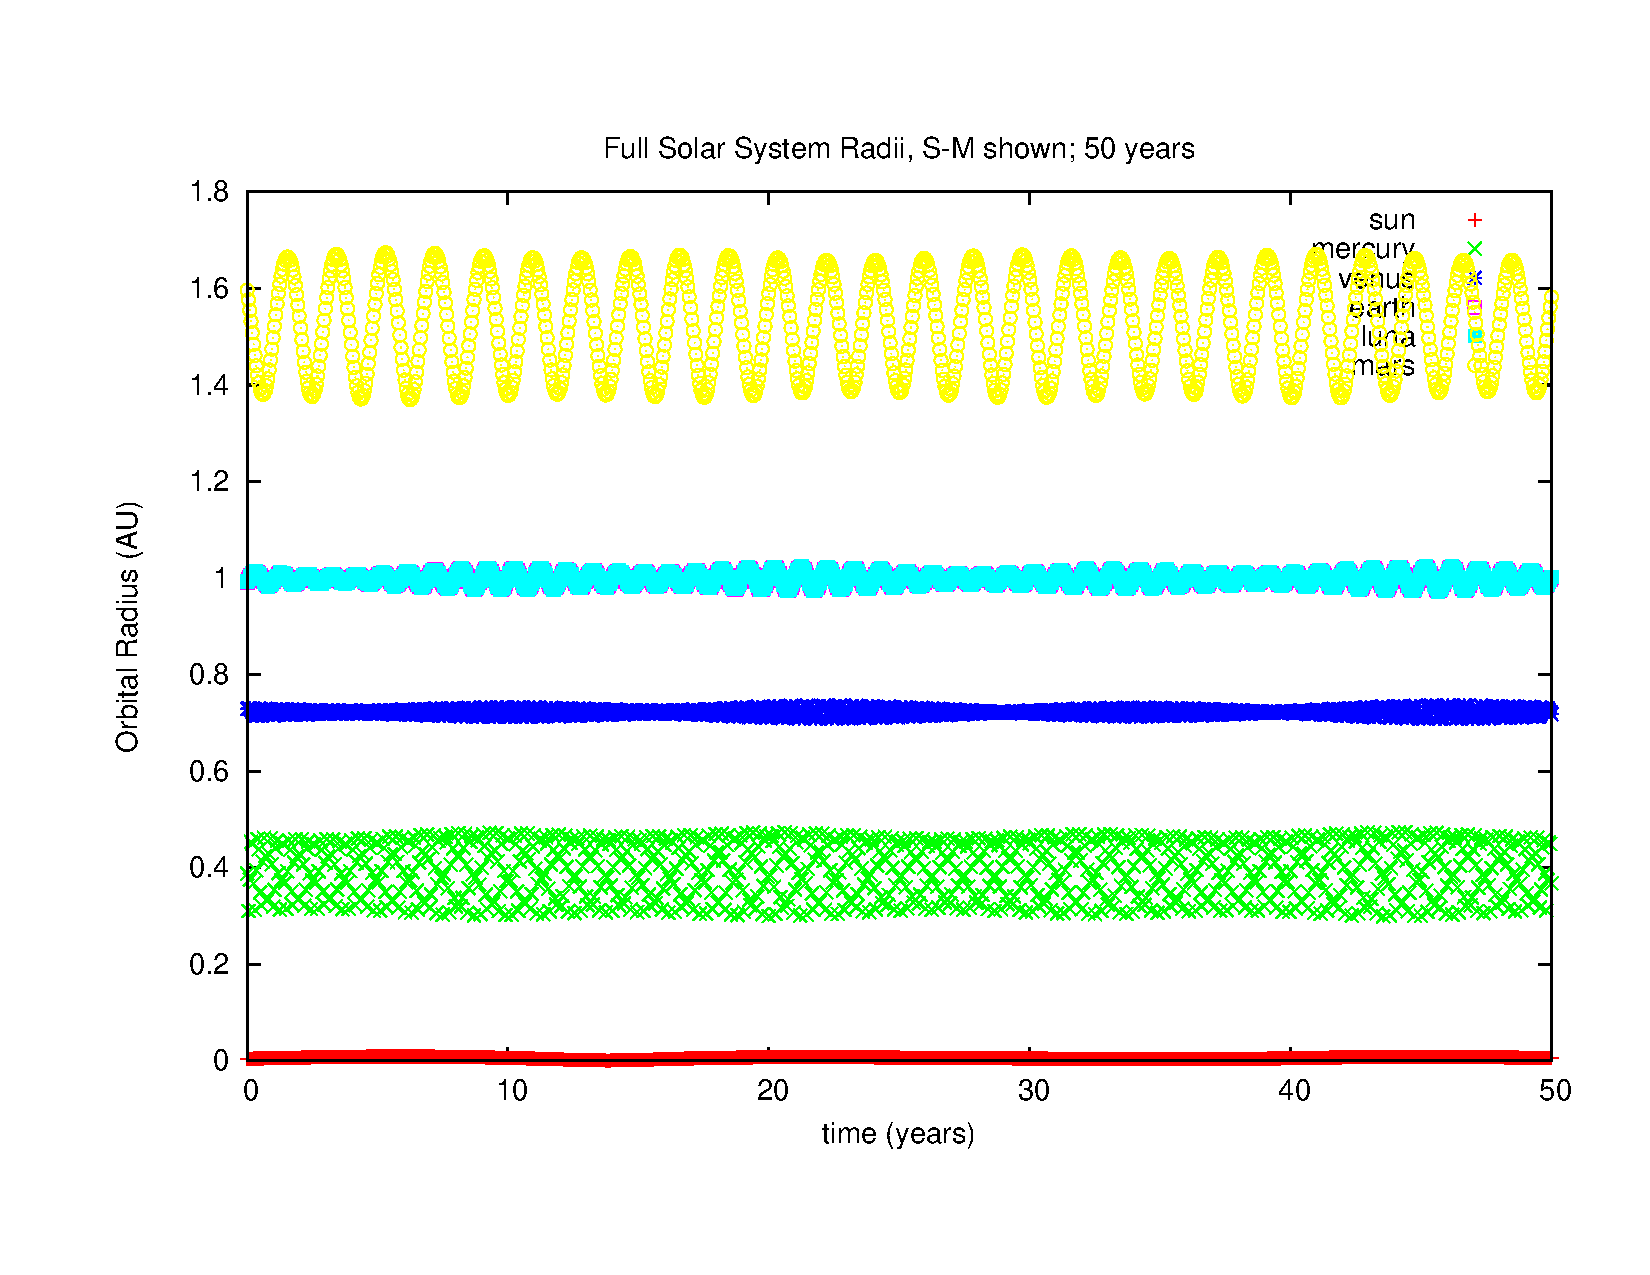
\includegraphics[width=1.0\textwidth]{fullss_radii_s-m_50years.pdf}
\caption{Here we see the evolution of the solar system over 50 years, where all bodies were used for the calculation but only the inner have been plotted for clarity. We plot the radii versus time in years to get a clear picture of the period and eccentricity of each body in the interior of the solar system. At this length scale we are able to discern each path clearly; however, due to the time scale the periods of mercury and venus are unclear. The data pulls them out clearly, but this graph has been prepared with a time scale sufficient to demonstrate their stability and the periodicity of their orbits.}
\end{figure}

\section{Discussion}

Here we discuss the computational speed and stability of the algorithms, as well as the effects of varying the initial velocity and the effects of other planets on the orbital path of the earth. 

We see clearly that the Verlet algorithm is not only faster but also in this particular implementation seems to propagate a lower error. Verlet runs in one-third the time and propagates error as $h^4$ as opposed with RK4's $h^3$. Further, the Verlet with relativistic corrections rights only slightly slower than the full Verlet algorithm with a slight improvement in error propagation. This is likely due to the necessity of approximating not only the position but also the velocity using the RK4 method. In simpler implementations, RK4 exceeds Verlet in accuracy. It should be noted that this is for the ideal case of circular motion with only the orbiting body being allowed to evolve, and these change as additional bodies are added and allowed to be mobile. The error propagation and relative speed remain similar; however, care must be taken for large systems since many, many more numerical evaluations will be required than for those with fewer bodies. This increase in the number of floating point operations will mean that, while the error propagates the same, the error will sum to be significant much sooner. Consider increasing the steps until a stable solution is found; then, optimize for computation time versus accuracy.

In the case of circular motion, we see that the orbital speed required for the earth for such a path is $2\pi \frac{AU}{yr}$ at a distance of one $AU$. As we increase the speed closer and closer to the escape velocity of $2sqrt(2)\pi \frac{AU}{yr}$, we observe that the orbit becomes more and more elliptical and the period increases. Once the speed is increased to $2\sqrt{2}\pi \frac{AU}{yr}$, the earth finally will escape and cease to orbit the sun.

With the additional of Jupiter to the system we see that the orbital of earth is only slightly perturbed. Instead of a perfectly circular orbit, we see deviations from this path due to Jupiter's sizeable mass, about one one-thousandth that of the sun. As we increase the mass of Jupiter tenfold, the perturbations become larger, but still relatively small. However, if we increase Jupiter's mass to one thousand times the original, near that of the sun, we see that earth suffers from a slingshot effect which ejects it from the solar system just after four years. 

Once all nine original planets and the earth's moon have been added for consideration, we see that the number of required steps increases. If the time under consideration is sufficiently small, one thousand steps per year suffices. If long periods of evolution are considered, such as many hundreds of years or several millenia, the required steps increase. Mercury is clearly the least stable since it has been the first ejected in all calculations performed in development of the code. The paths of each planet can be seen using a three dimensional plot, and the period of each orbit can be extracted from a radius versus time graph or from output option four. The solar system model is stable for millenia given sufficient steps, but computation time quickly increases to large values.

\section{Conclusion}

In this project we have developed code for calculating the evolution of a system of bodies given a set of initial positions and velocities, here specialized to the gravitational problem. We investigated the Verlet and Runge-Kutta methodologies for solving this system and found that, for this particular implementation of RK4, the Verlet algorithm requires one-third the time and fewer steps per year, propagating error as $h^4$ as opposed to $h^3$. Using these algorithms, we then applied the code to several variations of the solar system. We found that velocities required for the earth to have a circular orbit or to escape the sun's pull to be $2\pi$ and $2\sqrt{2}\pi \frac{AU}{yr}$, respectively. Further, we find that Jupiter adds only small perturbations to earth's orbit until its mass is increased to near that of the sun, at which point the earth escapes the system. Lastly, the solar system appears to be stable for several millenia as calcualted by this code, which bodes well for us all.

\section{References}

[1] M. Hjorth-Jensen. Computational Physics, lecture notes spring 2016. Department of Physics, Michigan State University, 2016. \newline
[2] Solar System Dynamics. Jet Propulsion Laboratory: California Institute of Technology.  [accessed 18 March 2016; ssd.jpl.nasa.gov/horizons.cgi] \newline

\newpage

\section*{Code Attachment}

\begin{lstlisting}[title={project3.cpp}]
/****************************************************
This code file solves the evolution of a system 
of massive bodies given their respective mass, 
positions, and velocities. In particular, we 
model the solar system given data from Nasa's Jet
Propulsion Laboratory. We proceed by two methods, 
Verlet and Runge Kutta to the fourth order. 


Verlet takes advantage of Taylor expansions, 
resulting in the following equations for the
positions and velocities:

x_i+1 = x_i + h*v_i + (h^2)/2*Force_i/mass
v_i+1 = v_i + (h/2)*(Force_i+1 + Force_i)/mass


RK4 uses Simpson's rule, that is
integral_(t)^(t+h) (f(x,t)) 
 = (h/6)*(f(i) + 4*f(i+1/2) + f(i+1))
 = (h/6)*(f(i) + 2*f(i+1/2) + 2*f(i+1/2) + f(i+1)
 = (h/6)*(k1 + 2*k2 + 2*k3 + k4),
where we define f(i) = f(x_i, t_i). In our case, 
we must perform this operation for both x and v, 
where we follow
 
	k1v = force(i)/mass
	k1x = v(i)
	x_i+1/2 = x(i) + (h/2)*k1x

	k2v = force(i+1/2)/mass
	k2x = v(i) + (h/2)*k2v
	x_i+1/2 = x(i) + (h/2)*k2x

	k3v = force(i+1/2)/mass
	k3x = v(i) + (h/2)*k3v
	x_i+1 = x(i) + h*k3x

	k4v = force(i+1)/mass
	k4x = v(i) + h*k4v

	v_i+1 = v(i) + (h/6)*(k1v + 2*k2v + 2*k3v + k4v)
	x_i+1 = x(i) + (h/6)*(k1x + 2*k2x + 2*k3x + k4x)


There is also the option to allow the system to
evolve using the first relativistic correction to the
force. The methods follow exactly as above once this
modification has been made to the force.

****************************************************/

#include<iostream>
#include<cmath>
#include<iomanip>
#include<fstream>
#include<string>
#include<sstream>
#include "time.h"
#include "project3_library.h"

using namespace std;

ofstream ofile, ofile2;

int main(int argc, char* argv[]){
	double** output, **aphelion, **perihelion;
	char* outfilename;

	int i, j, k, steps, planet_choice, sun_choice, method, outputtype, bodies;
	int stepsperyear, timesperyear;
	int dec_or_inc, aphguess, periguess;
	double tmax, time, timesort;

	clock_t start, finish;
	string periname, aphname;
	stringstream number;

	if(argc<8){
		cout << "Bad usage. Enter also 'outfilename planet_choice immobilize_sun_choice method_choice output_type steps tmax' on same line." << endl;
		cout << "Current options for planet_choice include" << endl;
		cout << "\t1: coplanar earth-sun system" << endl << "\t2: coplanar earth-jupiter-sun system" << endl;
		cout << "\t3: full solar system, with planets and luna" << endl;
		cout << "\t4: coplanar sun-mercury system" << endl << "\t5: rogue star full solar system, for fun" << endl;
		cout << "Current options for immobilze_sun_choice include" << endl;
		cout << "\t0: allow sun to evolve in coordinate space" << endl << "\t1: sun is initialized only and is not affected by other bodies" << endl;
		cout << "Current options for method_choice include" << endl;
		cout << "\t1: RK4" << endl << "\t2: Verlet" << endl << "\t3: non-class Verlet" << endl << "\t4: non-class relativistic Verlet" << endl;
		cout << "Current options for output_type include" << endl;
		cout << "\t1: pure output, steps by 8*bodies + 1" << endl << "\t2: as one, with print maximum aphelion and minimum perihelion to screen" << endl;
		cout << "\t3: 'timesperyear' ouput per earth year, enter after 'tmax'" << endl << "\t4: as three, with helionstates data files created" << endl;
		exit(1);
	}
	else{
		outfilename = argv[1];
		planet_choice = atoi(argv[2]);
		sun_choice = atoi(argv[3]);
		method = atoi(argv[4]);
		outputtype = atoi(argv[5]);
		steps = atoi(argv[6]);
		tmax = atof(argv[7]);
		if(outputtype==3||outputtype==4){
			if(argc<9){
				cout << "Bad usage. Enter also 'timesperyear' after 'tmax.'" << endl;
				exit(1);
			}
			tmax = atoi(argv[7]);
			timesperyear = atoi(argv[8]);
			if(timesperyear==0){
				cout << "Bad usage. Need a non-zero 'timesperyear.'" << endl;
				exit(1);
			}
			if(timesperyear*tmax>steps){
				cout << "Bad usage. 'timesperyear'*'tmax' is bigger than total 'steps.' Insufficient data points for output." << endl;
				exit(1);
			}
			stepsperyear = steps/(tmax*timesperyear);
		}	
	}
		
/********************************************
Here are the major massive bodies present 
within our solar system. Comment out any
which are not desired for the calculation.

Current options are
1: coplanar earth-sun system
2: coplanar earth-jupiter-sun system
3: full solar system, with planets and luna
4: coplanar sun-mercury system
5: rogue star full solar system, for fun
********************************************/

		massivesystem solarsystem;

	if(planet_choice==1){
		massivebody sun(1,0,0,0,0,0,0);
		massivebody earth(3.003489e-6,1,0,0,0,2.0*M_PI,0);
		solarsystem.add(sun);
		solarsystem.add(earth);
	}
	if(planet_choice==2){
		if(sun_choice==0){
			massivebody sun(1,-3.003489e-6,9.5479194e-4*5.2,0,-9.5479194e-4*0.439*2.0*M_PI,-3.003489e-6*2.0*M_PI,0);
			massivebody earth(3.003489e-6,1,0,0,0,2.0*M_PI,0);
			massivebody jupiter(9.5479194e-4,0,-5.2,0,0.439*2.0*M_PI,0,0);
			solarsystem.add(sun);
			solarsystem.add(earth);
			solarsystem.add(jupiter);
		}		
		if(sun_choice==1){
			massivebody sun(1,0,0,0,0,0,0);
			massivebody earth(3.003489e-6,1,0,0,0,2.0*M_PI,0);
			massivebody jupiter(9.5479194e-4,0,-5.2,0,0.439*2.0*M_PI,0,0);
			solarsystem.add(sun);
			solarsystem.add(earth);
			solarsystem.add(jupiter);
		}
	}
	if(planet_choice==3){
		massivebody sun(1,3.771551748320805E-03, 1.938413234187417E-03, -1.625928558000791E-04,365*3.428095941073785E-08, 365*6.978886434512168E-06, 365*-9.372671992938156E-09);
		massivebody mercury(1.6601e-7,3.566221110752382E-01,-1.449153604767920E-01,-4.453344798939488E-02, 365*5.324168987021533E-03,365*2.725352157519689E-02, 365*1.737877336062238E-03);
		massivebody venus(2.4478383e-6,4.456189829066335E-01,-5.759198980424926E-01,-3.358283335789598E-02,365*1.593371764525070E-02, 365*1.222110108236829E-02,365*-7.520174121955455E-04);
		massivebody earth(3.003489e-6,-9.906650404586314E-01,4.353612431574581E-02,-1.569714899841466E-04,365*-9.933032846586867E-04,365*-1.724423592380582E-02,365*2.880574493748607E-07);
		massivebody moon(1.230004e-8, -9.917828800119005E-01, 4.587463373520608E-02, -3.563694480647205E-04, 365*-1.530892843498182E-03, 365*-1.746686609878291E-02, 365*2.803200805250705E-05);
		massivebody mars(3.227151e-7, -1.394909885799664E+00, -7.759974369033253E-01, 1.786251125355763E-02, 365*7.324673346484570E-03, 365*-1.102624283521118E-02, 365*-4.109846883854566E-04);
		massivebody jupiter(9.5479194e-4,-5.321136962878863E+00, 1.055810040982731E+00, 1.146123452783326E-01, 365*-1.556597232697437E-03, 365*-7.046207863842619E-03, 365*6.409351264039102E-05);
		massivebody saturn(2.858860e-4,-3.332098484988519E+00, -9.442038663142483E+00, 2.967846224795282E-01, 365*4.954645896896637E-03, 365*-1.873255191158998E-03, 365*-1.647257228743735E-04);
		massivebody uranus(4.366244e-5, 1.876841090026478E+01, 6.826065082612249E+00, -2.177966843356428E-01, 365*-1.372937790621792E-03, 365*3.512867479374193E-03, 365*3.086802162915850E-05);
		massivebody neptune(5.151389e-5, 2.803900494548452E+01, -1.054870089186826E+01, -4.289565554838171E-01, 365*1.084650993604757E-03, 365*2.957157649376530E-03, 365*-8.562727609311126E-05);
		massivebody pluto(6.5812e-9, 8.773368933896196E+00, -3.186331328356860E+01, 8.718065633574812E-01, 365*3.100891963853092E-03, 365*1.939401372093854E-04, 365*-9.194995916567601E-04);

		solarsystem.add(sun);
		solarsystem.add(mercury);
		solarsystem.add(venus);
		solarsystem.add(earth);
		solarsystem.add(moon);
		solarsystem.add(mars);
		solarsystem.add(jupiter);
		solarsystem.add(saturn);
		solarsystem.add(uranus);
		solarsystem.add(neptune);
		solarsystem.add(pluto);
	}
	if(planet_choice==4){
		massivebody sun(1,0,0,0,0,0,0);
		massivebody mercury(1.6601e-7,0.3075, 0, 0, 0, 12.44, 0);
	
		solarsystem.add(sun);
		solarsystem.add(mercury);
	}
	if(planet_choice==5){

		massivebody sun(1,3.771551748320805E-03, 1.938413234187417E-03, -1.625928558000791E-04,365*3.428095941073785E-08, 365*6.978886434512168E-06, 365*-9.372671992938156E-09);
		massivebody mercury(1.6601e-7,3.566221110752382E-01,-1.449153604767920E-01,-4.453344798939488E-02, 365*5.324168987021533E-03,365*2.725352157519689E-02, 365*1.737877336062238E-03);
		massivebody venus(2.4478383e-6,4.456189829066335E-01,-5.759198980424926E-01,-3.358283335789598E-02,365*1.593371764525070E-02, 365*1.222110108236829E-02,365*-7.520174121955455E-04);
		massivebody earth(3.003489e-6,-9.906650404586314E-01,4.353612431574581E-02,-1.569714899841466E-04,365*-9.933032846586867E-04,365*-1.724423592380582E-02,365*2.880574493748607E-07);
		massivebody moon(1.230004e-8, -9.917828800119005E-01, 4.587463373520608E-02, -3.563694480647205E-04, 365*-1.530892843498182E-03, 365*-1.746686609878291E-02, 365*2.803200805250705E-05);
		massivebody mars(3.227151e-7, -1.394909885799664E+00, -7.759974369033253E-01, 1.786251125355763E-02, 365*7.324673346484570E-03, 365*-1.102624283521118E-02, 365*-4.109846883854566E-04);
		massivebody jupiter(9.5479194e-4,-5.321136962878863E+00, 1.055810040982731E+00, 1.146123452783326E-01, 365*-1.556597232697437E-03, 365*-7.046207863842619E-03, 365*6.409351264039102E-05);
		massivebody saturn(2.858860e-4,-3.332098484988519E+00, -9.442038663142483E+00, 2.967846224795282E-01, 365*4.954645896896637E-03, 365*-1.873255191158998E-03, 365*-1.647257228743735E-04);
		massivebody uranus(4.366244e-5, 1.876841090026478E+01, 6.826065082612249E+00, -2.177966843356428E-01, 365*-1.372937790621792E-03, 365*3.512867479374193E-03, 365*3.086802162915850E-05);
		massivebody neptune(5.151389e-5, 2.803900494548452E+01, -1.054870089186826E+01, -4.289565554838171E-01, 365*1.084650993604757E-03, 365*2.957157649376530E-03, 365*-8.562727609311126E-05);
		massivebody pluto(6.5812e-9, 8.773368933896196E+00, -3.186331328356860E+01, 8.718065633574812E-01, 365*3.100891963853092E-03, 365*1.939401372093854E-04, 365*-9.194995916567601E-04);
		massivebody roguestar(1,-500,0,0,50,0,0);

		solarsystem.add(sun);
		solarsystem.add(mercury);
		solarsystem.add(venus);
		solarsystem.add(earth);
		solarsystem.add(moon);
		solarsystem.add(mars);
		solarsystem.add(jupiter);
		solarsystem.add(saturn);
		solarsystem.add(uranus);
		solarsystem.add(neptune);
		solarsystem.add(pluto);
		solarsystem.add(roguestar);
	}

	bodies = solarsystem.massivebody_count;
	matrix_alloc(output, steps+1, bodies*8+1);

/**********************************************
method choice
	1: RK4
	2: Verlet
	3: Non-massivesystem Verlet
	4: Verlet with relativistic correction
**********************************************/
	if(method==1){
		start = clock();
		solarsystem.RK4(output,steps,tmax,sun_choice);
		finish = clock();
	}
	else if(method==2){
		start = clock();
		solarsystem.verlet(output,steps,tmax,sun_choice);
		finish = clock();
	}
	else if(method==3){
		double* mass = new double[bodies];
		start = clock();
		solarsystem.initialize(output, mass, steps);
		verlet(output,mass,bodies,steps,tmax,sun_choice);
		finish = clock();
		delete[] mass;
	}
	else if(method==4){
		double* mass = new double[bodies];
		start = clock();
		solarsystem.initialize(output, mass, steps);
		verlet_relcor(output,mass,bodies,steps,tmax,sun_choice);
		finish = clock();
		delete[] mass;
	}
	time = (finish - start)/((double) CLOCKS_PER_SEC);

/*****************************************************************
outputfile choice
	1: Pure output file. No modifications
	2: As one, but with the largest and smallest, respectively, 
		aphelion and perihelion for each body printed to screen
	3: Output 'timesperyear' data points per year, for long 
		time spans
	4: As two, but with data files for each body containing all 
		aphelion and perilion positions
*****************************************************************/

	ofile.open(outfilename);
	ofile.precision(8);
	if(outputtype==1){
		start = clock();
		for(i=0;i<steps+1;i++){
			for(j=0;j<bodies*8+1;j++){
				ofile << setw(15) << output[i][j];
			}
			ofile << endl;
		}
		finish = clock();
	}
	else if(outputtype==2){
		start = clock();
		matrix_alloc(aphelion,bodies,2);
		matrix_alloc(perihelion,bodies,2);
		for(i=0;i<steps+1;i++){
			for(j=0;j<bodies*8+1;j++){
				ofile << setw(15) << output[i][j];
			}
			ofile << endl;
		}
		helionstates(output, aphelion, perihelion, bodies, steps);
		for(i=0;i<bodies;i++){
				cout << setw(15) << aphelion[i][0] << setw(15) << aphelion[i][1];
				cout << setw(30) << perihelion[i][0] << setw(15) << perihelion[i][1];
				cout << endl;
		}
		matrix_delete(aphelion,bodies);
		matrix_delete(perihelion,bodies);
		finish = clock();
	}
	else if(outputtype==3){
		start = clock();
		for(i=0;i<steps+1;i+=stepsperyear){
			for(j=0;j<bodies*8+1;j++){
				ofile << setw(15) << output[i][j];
			}
			ofile << endl;
		}
		finish = clock();
	}
	else if(outputtype==4){
		start = clock();
		for(i=0;i<steps+1;i+=stepsperyear){
			for(j=0;j<bodies*8+1;j++){
				ofile << setw(15) << output[i][j];
			}
			ofile << endl;
		}
		for(k=0;k<bodies;k++){
			periname = "perihelion_body_";
			aphname = "aphelion_body_";
			aphguess = 1;
			periguess = aphguess;
			number << k;
			periname += number.str() + ".dat";
			aphname += number.str() + ".dat";
			number.str("");
			matrix_alloc(aphelion,aphguess,5);
			matrix_alloc(perihelion,periguess,5);
			dec_or_inc=1;
			helionstates_dynamic(aphelion, aphguess, perihelion, periguess, output,steps,k,20,dec_or_inc);
			
			ofile2.open(periname);
			ofile2.precision(8);
			for(i=0;i<periguess;i++){
				for(j=0;j<5;j++){
					ofile2 << setw(15) << perihelion[i][j];
				}
				ofile2 << endl;
			}
			ofile2.close();
			ofile2.open(aphname);
			ofile2.precision(8);
			for(i=0;i<aphguess;i++){
				for(j=0;j<5;j++){
					ofile2 << setw(15) << aphelion[i][j];
				}
				ofile2 << endl;
			}
			ofile2.close();

			matrix_delete(aphelion,aphguess);
			matrix_delete(perihelion,periguess);
		}
		finish = clock();
	}
	timesort = (finish - start)/((double) CLOCKS_PER_SEC);

	//print time for calculation to screen
	cout << "\tcomputation time " << time << " seconds" << endl;
	cout << "\toutput time " << timesort << " seconds" << endl;
	ofile.close();

	matrix_delete(output,steps+1);
	return 0;
}
\end{lstlisting}
\begin{lstlisting}[title={project3-library.h}]
#ifndef PROJECT3_LIBRARY_H
#define PROJECT3_LIBRARY_H

#include<iostream>
#include<cmath>
#include<iomanip>
#include<fstream>

using namespace std;

//massivebody contains the mass, positions, and velocities
//a constructor with a "primary" massivebody is given to create
//	an orbiting mass around said "primary"
class massivebody{
	public:
		double mass;
		double position[4];
		double velocity[4];
		massivebody();
		massivebody(double, double, double, double, double, double, double);
		massivebody(massivebody, double, double, double, double, double, double, double);
};

//massivesystem contains all necessary components to solve for evolution
//massivebody_count tracks the size of massivebody* system
//the total mass and Center of Mass positions & velocities are given via
//	mass_total, composition[4], comvelocity[4]
//after defining a massive system, 'add' resizes massivebody* and tacks the
//	new massivebody onto the end
class massivesystem{
	public:
		int massivebody_count;
		massivebody* system;
		double mass_total;
		double composition[4];
		double comvelocity[4];

		massivesystem();
		~massivesystem();

		void add(massivebody guy);
		void update(double**&, int);
		void relpositions(double**&);
		void forces(double*&, const double**&);
		void initialize(double**&, double*&, int);
		void verlet(double**&, int, double, int);
		void RK4(double**&, int, double, int);
		void print();
};
class vector{
	public:
		int length;
		double* array;
};

inline void array_alloc(double*& a, int length);
inline void array_delete(double*& a);
inline void array_resize(double*&, int, int);
inline void matrix_alloc(double**&, int, int);
inline void matrix_delete(double**&, int);
inline void matrix_resize(double**&, int, int, int, int);
inline void threeDarray_alloc(double***& a, int d1, int d2, int d3);
inline void threeDarray_delete(double***& a, int d1, int d2);
inline void rel_position(double**&, double**&, int, int);
inline void rel_coord(double**&, double**&, int, int);
inline void rel_angmomentum(double**&, double**&, int);
inline void gravityforces(double**&, double**&, double*&, int, int);
inline void gravityforces_relcorrection(double**&, double**&, double**&, double*&, int, int);
void verlet(double**&, double*&, int, int, double, int);
void verlet_relcor(double**&, double*&, int, int, double, int);
void helionstates(double**&, double**&, double**&, int, int);
void helionstates_dynamic(double**& aphelion, int& aphguess, double**& perihelion, int& periguess, double**& output, int steps, int body, int range, int dec_or_inc);

/**************************
Begin function definitions
***************************/


/*********************
massivebody functions
*********************/
massivebody::massivebody(){
	mass = 0.0;
	position[0] = 0.0;
	position[1] = 0.0;
	position[2] = 0.0;
	position[3] = 0.0;
	velocity[0] = 0.0;
	velocity[1] = 0.0;
	velocity[2] = 0.0;
	velocity[3] = 0.0;
}
massivebody::massivebody(double Mass, double x, double y, double z, double vx, double vy, double vz){
	mass = Mass;
	position[0] = x;
	position[1] = y;
	position[2] = z;
	position[3] = sqrt(position[0]*position[0] + position[1]*position[1] + position[2]*position[2]);
	velocity[0] = vx;
	velocity[1] = vy;
	velocity[2] = vz;
	velocity[3] = sqrt(vx*vx + vy*vy + vz*vz);
}
massivebody::massivebody(massivebody primary, double Mass, double x, double y, double z, double vx, double vy, double vz){
	mass = Mass;
	position[0] = primary.position[0] + x;
	position[1] = primary.position[1] + y;
	position[2] = primary.position[2] + z;
	position[3] = sqrt(position[0]*position[0] + position[1]*position[1] + position[2]*position[2]);
	velocity[0] = primary.velocity[0] + vx;
	velocity[1] = primary.velocity[1] + vy;
	velocity[2] = primary.velocity[2] + vz;
	velocity[3] = sqrt(velocity[0]*velocity[0] + velocity[1]*velocity[1] + velocity[2]*velocity[2]);
}

/***********************
massivesystem functions
***********************/
massivesystem::massivesystem(){
	massivebody_count = 0;
	system = nullptr;
	mass_total = 0;
	for(int i=0;i<4;i++){
		composition[i]=0.0;
		comvelocity[i]=0.0;
	}
}
massivesystem::~massivesystem(){
	delete[] system;
}
void massivesystem::add(massivebody guy){
	double mass_old = mass_total;
	massivebody* temp = new massivebody[massivebody_count+1];
	for(int i=0;i<massivebody_count;i++){
		temp[i].mass=system[i].mass;
		temp[i].position[0]=system[i].position[0];
		temp[i].position[1]=system[i].position[1];
		temp[i].position[2]=system[i].position[2];
		temp[i].position[3]=system[i].position[3];
		temp[i].velocity[0]=system[i].velocity[0];
		temp[i].velocity[1]=system[i].velocity[1];
		temp[i].velocity[2]=system[i].velocity[2];
		temp[i].velocity[3]=system[i].velocity[3];
	}
	temp[massivebody_count].mass=guy.mass;
	temp[massivebody_count].position[0]=guy.position[0];
	temp[massivebody_count].position[1]=guy.position[1];
	temp[massivebody_count].position[2]=guy.position[2];
	temp[massivebody_count].position[3]=guy.position[3];
	temp[massivebody_count].velocity[0]=guy.velocity[0];
	temp[massivebody_count].velocity[1]=guy.velocity[1];
	temp[massivebody_count].velocity[2]=guy.velocity[2];
	temp[massivebody_count].velocity[3]=guy.velocity[3];

	massivebody_count++;

	delete[] system;
	mass_total += guy.mass;
	for(int i=0;i<3;i++){
		composition[i] = (composition[i]*mass_old + guy.position[i]*guy.mass)/mass_total;
		comvelocity[i] = (comvelocity[i]*mass_old + guy.velocity[i]*guy.mass)/mass_total;
	}
	composition[3] = sqrt(composition[0]*composition[0] + composition[1]*composition[1] + composition[2]*composition[2]);
	comvelocity[3] = sqrt(comvelocity[0]*comvelocity[0] + comvelocity[1]*comvelocity[1] + comvelocity[2]*comvelocity[2]);
	system = temp;
}
void massivesystem::update(double**& output, int i){
	int j;
	mass_total = 0.0;
	for(j=0;j<4;j++){
		composition[j] = 0.0;
		comvelocity[j] = 0.0;
	}

	for(j=0;j<massivebody_count;j++){
		system[j].position[0] = output[i][8*j+1];
		system[j].position[1] = output[i][8*j+2];
		system[j].position[2] = output[i][8*j+3];
		system[j].position[3] = output[i][8*j+4];
		system[j].velocity[0] = output[i][8*j+5];
		system[j].velocity[1] = output[i][8*j+6];
		system[j].velocity[2] = output[i][8*j+7];
		system[j].velocity[3] = output[i][8*j+8];
		mass_total += system[j].mass;
	}
	for(j=0;j<massivebody_count;j++){
		composition[0] += system[j].position[0]*system[j].mass;
		composition[1] += system[j].position[1]*system[j].mass;
		composition[2] += system[j].position[2]*system[j].mass;
		comvelocity[0] += system[j].velocity[0]*system[j].mass;
		comvelocity[1] += system[j].velocity[1]*system[j].mass;
		comvelocity[2] += system[j].velocity[2]*system[j].mass;
	}
	comvelocity[0] /= mass_total;
	comvelocity[1] /= mass_total;
	comvelocity[2] /= mass_total;

	composition[3] = sqrt(composition[0]*composition[0] + composition[1]*composition[1] + composition[2]*composition[2]);
	comvelocity[3] = sqrt(comvelocity[0]*comvelocity[0] + comvelocity[1]*comvelocity[1] + comvelocity[2]*comvelocity[2]);
}
void massivesystem::print(){
	cout << "mass=" << setw(15) << mass_total << endl;
	cout << "body_count=" << setw(15) << massivebody_count << endl;
	for(int i=0;i<4;i++){
		cout << "pos[" << i<< "]=" << setw(15) << composition[i] << endl;
	}
	for(int i=0;i<4;i++){
		cout << "vel[" << i<< "]=" << setw(15) << comvelocity[i] << endl;
	}
}
void massivesystem::relpositions(double**& relcoord){
	int i, j;	
	int bodies = massivebody_count;
	for(i=0;i<bodies;i++){
		for(j=0;j<bodies;j++){
			if(i!=j){
				relcoord[i][j*4] = system[i].position[0] - system[j].position[0];
				relcoord[i][j*4+1] = system[i].position[1] - system[j].position[1];
				relcoord[i][j*4+2] = system[i].position[2] - system[j].position[2];
				relcoord[i][j*4+3] = sqrt(relcoord[i][j*4]*relcoord[i][j*4] + relcoord[i][j*4+1]*relcoord[i][j*4+1]+relcoord[i][j*4+2]*relcoord[i][j*4+2]);
			}
		}
	}
}
void massivesystem::forces(double*& force, const double**& relcoord){
	int j, k;
	int bodies = massivebody_count;
	double rcubed, fourpisq;
	fourpisq = 4.0*M_PI*M_PI;
	for(j=0;j<bodies;j++){
		force[j*3] = 0.0;
		force[j*3+1] = 0.0;
		force[j*3+2] = 0.0;
	}
	for(j=0;j<bodies;j++){
		for(k=0;k<bodies;k++){
			if(j!=k){
				rcubed = pow(relcoord[j][k*4+3],3.0);
				force[j*3] += -system[k].mass*relcoord[j][k*4]/rcubed;
				force[j*3+1] += -system[k].mass*relcoord[j][k*4+1]/rcubed;
				force[j*3+2] += -system[k].mass*relcoord[j][k*4+2]/rcubed;
			}
		}
		force[j*3] *= fourpisq;
		force[j*3+1] *= fourpisq;
		force[j*3+2] *= fourpisq;
	}
}
void massivesystem::initialize(double**& output, double*& mass, int steps){
	int i, j;
	int bodies = massivebody_count;
	output = new double*[steps+1];
	mass = new double[bodies];
	for(int i=0;i<steps+1;i++){
		output[i] = new double[bodies*8+1];
	}
	for(i=1;i<steps+1;i++){
		for(j=0;j<bodies;j++){
			output[i][j*8+1] = 0;
			output[i][j*8+2] = 0;
			output[i][j*8+3] = 0;
			output[i][j*8+4] = 0;
			output[i][j*8+5] = 0;
			output[i][j*8+6] = 0;
			output[i][j*8+7] = 0;
			output[i][j*8+8] = 0;
		}
	}
	for(j=0;j<bodies;j++){
		mass[j] = system[j].mass;
		output[0][j*8+1] = system[j].position[0];
		output[0][j*8+2] = system[j].position[1];
		output[0][j*8+3] = system[j].position[2];
		output[0][j*8+4] = system[j].position[3];
		output[0][j*8+5] = system[j].velocity[0];
		output[0][j*8+6] = system[j].velocity[1];
		output[0][j*8+7] = system[j].velocity[2];
		output[0][j*8+8] = system[j].velocity[3];
	}
}


/***************************
class function solvers,
RK4 and Verlet
***************************/
void massivesystem::RK4(double**& output, int steps, double tmax, int sun_choice){
	int i, j, k, m, n, bodies;
	bodies = massivebody_count;
	double h, halfh, halfhsq, rcubed, fourpisq;
	double* k2, *k3;
	h = (tmax-0.0)/((double) (steps));
	halfh = 0.5*h;
	halfhsq = halfh*h;	
	fourpisq = 4.0*M_PI*M_PI;

	//placeholders arrays
	k2 = new double[bodies*6];
	k3 = new double[bodies*6];
	for(i=0;i<bodies*6;i++){
		k2[i] = 0;
		k3[i] = 0;
	}
	//relcoord to provide relative coordinates, x, y, z, r, of body i with respect to body j
	double** relcoord = new double*[bodies];
	for(i=0;i<bodies;i++){
		relcoord[i] = new double[bodies*4];
	}
	//force provides fx,fy,fz for each body at step i and i+1
	double** force = new double*[2];
	for(i=0;i<2;i++){
		force[i] = new double[bodies*3];
	}
	//initialize all matrices to zero
	for(i=0;i<steps+1;i++){
		for(j=0;j<bodies*8+1;j++){
			output[i][j]=0.0;
		}
	}
	for(i=0;i<bodies;i++){
		for(j=0;j<bodies*4;j++){
			relcoord[i][j]=0.0;
		}
	}
	for(i=0;i<2;i++){
		for(j=0;j<bodies*3;j++){
			force[i][j]=0.0;
		}
	}

	//reinitialize relcoord to initial conditions
	//technically double calculating--consider revising
	for(i=0;i<bodies;i++){
		for(j=0;j<bodies;j++){
			if(i!=j){
				relcoord[i][j*4] = system[i].position[0] - system[j].position[0];
				relcoord[i][j*4+1] = system[i].position[1] - system[j].position[1];
				relcoord[i][j*4+2] = system[i].position[2] - system[j].position[2];
				relcoord[i][j*4+3] = sqrt(relcoord[i][j*4]*relcoord[i][j*4] + relcoord[i][j*4+1]*relcoord[i][j*4+1]+relcoord[i][j*4+2]*relcoord[i][j*4+2]);
			}
		}
	}
	//initialize forces (k1v)
	for(j=0;j<bodies;j++){
		for(k=0;k<bodies;k++){
			if(j!=k){
				rcubed = pow(relcoord[j][k*4+3],3.0);
				force[0][j*3] += -system[k].mass*relcoord[j][k*4]/rcubed;
				force[0][j*3+1] += -system[k].mass*relcoord[j][k*4+1]/rcubed;
				force[0][j*3+2] += -system[k].mass*relcoord[j][k*4+2]/rcubed;
			}
		}
		force[0][j*3] *= fourpisq;
		force[0][j*3+1] *= fourpisq;
		force[0][j*3+2] *= fourpisq;
	}
	//initialize initial conditions for output
	for(j=0;j<bodies;j++){
		output[0][j*8+1] = system[j].position[0];
		output[0][j*8+2] = system[j].position[1];
		output[0][j*8+3] = system[j].position[2];
		output[0][j*8+4] = system[j].position[3];
		output[0][j*8+5] = system[j].velocity[0];
		output[0][j*8+6] = system[j].velocity[1];
		output[0][j*8+7] = system[j].velocity[2];
		output[0][j*8+8] = system[j].velocity[3];
	}

	//Begin RK4 loop
	for(i=0;i<steps;i++){
		output[i+1][0] = output[i][0] + h;
		//calculate first positions [1+1/2]
		// (using k1x)
		for(j=sun_choice;j<bodies;j++){
			output[i+1][j*8+1] = output[i][j*8+1] + halfh*output[i][j*8+5];
			output[i+1][j*8+2] = output[i][j*8+2] + halfh*output[i][j*8+6];
			output[i+1][j*8+3] = output[i][j*8+3] + halfh*output[i][j*8+7];
		}
		//new relative positions at [i+1/2]
		for(m=0;m<bodies;m++){
			for(n=0;n<bodies;n++){
				if(m!=n){
					relcoord[m][n*4] = output[i+1][m*8+1] - output[i+1][n*8+1];
					relcoord[m][n*4+1] = output[i+1][m*8+2] - output[i+1][n*8+2];
					relcoord[m][n*4+2] = output[i+1][m*8+3] - output[i+1][n*8+3];
					relcoord[m][n*4+3] = sqrt(relcoord[m][n*4]*relcoord[m][n*4] + relcoord[m][n*4+1]*relcoord[m][n*4+1]+relcoord[m][n*4+2]*relcoord[m][n*4+2]);
				}
			}
		}
		//new forces with relative positions
		for(j=0;j<bodies*3;j++){
			force[1][j] = 0.0;
		}
		for(j=0;j<bodies;j++){
			for(k=0;k<bodies;k++){
				if(j!=k){
					rcubed = pow(relcoord[j][k*4+3],3.0);
					force[1][j*3] += -system[k].mass*relcoord[j][k*4]/rcubed;
					force[1][j*3+1] += -system[k].mass*relcoord[j][k*4+1]/rcubed;
					force[1][j*3+2] += -system[k].mass*relcoord[j][k*4+2]/rcubed;
				}
			}
			force[1][j*3] *= fourpisq;
			force[1][j*3+1] *= fourpisq;
			force[1][j*3+2] *= fourpisq;
			//k2v
			k2[j*6+3] = force[1][j*3];
			k2[j*6+4] = force[1][j*3+1];
			k2[j*6+5] = force[1][j*3+2];
		}
		//k2x using i+1/2 positions
		for(j=0;j<bodies;j++){
			k2[j*6] = output[i][j*8+5] + halfh*force[1][j*3];
			k2[j*6+1] = output[i][j*8+6] + halfh*force[1][j*3+1];
			k2[j*6+2] = output[i][j*8+7] + halfh*force[1][j*3+2];
		}
		//new temp positions at i+1/2 with k2x
		for(j=sun_choice;j<bodies;j++){
			output[i+1][j*8+1] = output[i][j*8+1] + halfh*k2[j*6];
			output[i+1][j*8+2] = output[i][j*8+2] + halfh*k2[j*6+1];
			output[i+1][j*8+3] = output[i][j*8+3] + halfh*k2[j*6+2];
		}
		//new relative positions at [i+1/2] with k2x
		for(m=0;m<bodies;m++){
			for(n=0;n<bodies;n++){
				if(m!=n){
					relcoord[m][n*4] = output[i+1][m*8+1] - output[i+1][n*8+1];
					relcoord[m][n*4+1] = output[i+1][m*8+2] - output[i+1][n*8+2];
					relcoord[m][n*4+2] = output[i+1][m*8+3] - output[i+1][n*8+3];
					relcoord[m][n*4+3] = sqrt(relcoord[m][n*4]*relcoord[m][n*4] + relcoord[m][n*4+1]*relcoord[m][n*4+1]+relcoord[m][n*4+2]*relcoord[m][n*4+2]);
				}
			}
		}
		//new forces with relative positions
		for(j=0;j<bodies*3;j++){
			force[1][j] = 0.0;
		}
		for(j=0;j<bodies;j++){
			for(k=0;k<bodies;k++){
				if(j!=k){
					rcubed = pow(relcoord[j][k*4+3],3.0);
					force[1][j*3] += -system[k].mass*relcoord[j][k*4]/rcubed;
					force[1][j*3+1] += -system[k].mass*relcoord[j][k*4+1]/rcubed;
					force[1][j*3+2] += -system[k].mass*relcoord[j][k*4+2]/rcubed;
				}
			}
			force[1][j*3] *= fourpisq;
			force[1][j*3+1] *= fourpisq;
			force[1][j*3+2] *= fourpisq;
			//k3v
			k3[j*6+3] = force[1][j*3];
			k3[j*6+4] = force[1][j*3+1];
			k3[j*6+5] = force[1][j*3+2];
		}
		//k3x using i+1/2 positions
		for(j=0;j<bodies;j++){
			k3[j*6] = output[i][j*8+5] + halfh*force[1][j*3];
			k3[j*6+1] = output[i][j*8+6] + halfh*force[1][j*3+1];
			k3[j*6+2] = output[i][j*8+7] + halfh*force[1][j*3+2];
		}
		//new temp positions at i+1 using k3x
		for(j=sun_choice;j<bodies;j++){
			output[i+1][j*8+1] = output[i][j*8+1] + h*k3[j*6];
			output[i+1][j*8+2] = output[i][j*8+2] + h*k3[j*6+1];
			output[i+1][j*8+3] = output[i][j*8+3] + h*k3[j*6+2];
		}
		//new relative positions at [i+1] with k3x
		for(m=0;m<bodies;m++){
			for(n=0;n<bodies;n++){
				if(m!=n){
					relcoord[m][n*4] = output[i+1][m*8+1] - output[i+1][n*8+1];
					relcoord[m][n*4+1] = output[i+1][m*8+2] - output[i+1][n*8+2];
					relcoord[m][n*4+2] = output[i+1][m*8+3] - output[i+1][n*8+3];
					relcoord[m][n*4+3] = sqrt(relcoord[m][n*4]*relcoord[m][n*4] + relcoord[m][n*4+1]*relcoord[m][n*4+1]+relcoord[m][n*4+2]*relcoord[m][n*4+2]);
				}
			}
		}
		//new forces with relative positions
		for(j=0;j<bodies*3;j++){
			force[1][j] = 0.0;
		}
		for(j=0;j<bodies;j++){
			for(k=0;k<bodies;k++){
				if(j!=k){
					rcubed = pow(relcoord[j][k*4+3],3.0);
					force[1][j*3] += -system[k].mass*relcoord[j][k*4]/rcubed;
					force[1][j*3+1] += -system[k].mass*relcoord[j][k*4+1]/rcubed;
					force[1][j*3+2] += -system[k].mass*relcoord[j][k*4+2]/rcubed;
				}
			}
			force[1][j*3] *= fourpisq;
			force[1][j*3+1] *= fourpisq;
			force[1][j*3+2] *= fourpisq;
		}
		//k4x using i+1/2 positions
		for(j=sun_choice;j<bodies;j++){
			output[i+1][j*8+5] = output[i][j*8+5] + h*force[1][j*3];
			output[i+1][j*8+6] = output[i][j*8+6] + h*force[1][j*3+1];
			output[i+1][j*8+7] = output[i][j*8+7] + h*force[1][j*3+2];
		}
		//final positions at i+1
		for(j=sun_choice;j<bodies;j++){
			output[i+1][j*8+1] = output[i][j*8+1] + (h/6.0)*(output[i][j*8+5] + 2.0*k2[j*6] + 2.0*k3[j*6] + output[i+1][j*8+5]);
			output[i+1][j*8+2] = output[i][j*8+2] + (h/6.0)*(output[i][j*8+6] + 2.0*k2[j*6+1] + 2.0*k3[j*6+1] + output[i+1][j*8+6]);
			output[i+1][j*8+3] = output[i][j*8+3] + (h/6.0)*(output[i][j*8+7] + 2.0*k2[j*6+2] + 2.0*k3[j*6+2] + output[i+1][j*8+7]);
			output[i+1][j*8+4] = sqrt(output[i+1][j*8+1]*output[i+1][j*8+1] + output[i+1][j*8+2]*output[i+1][j*8+2] + output[i+1][j*8+3]*output[i+1][j*8+3]);
		}	
		//final velocities at i+1
		for(j=sun_choice;j<bodies;j++){
			output[i+1][j*8+5] = output[i][j*8+5] + (h/6.0)*(force[0][j*3] + 2.0*k2[j*6+3] + 2.0*k3[j*6+3] + force[1][j*3]);
			output[i+1][j*8+6] = output[i][j*8+6] + (h/6.0)*(force[0][j*3+1] + 2.0*k2[j*6+4] + 2.0*k3[j*6+4] + force[1][j*3+1]);
			output[i+1][j*8+7] = output[i][j*8+7] + (h/6.0)*(force[0][j*3+2] + 2.0*k2[j*6+5] + 2.0*k3[j*6+5] + force[1][j*3+2]);
			output[i+1][j*8+8] = sqrt(output[i+1][j*8+5]*output[i+1][j*8+5] + output[i+1][j*8+6]*output[i+1][j*8+6] + output[i+1][j*8+7]*output[i+1][j*8+7]);
		}
		//final relative positions at i+1
		for(m=0;m<bodies;m++){
			for(n=0;n<bodies;n++){
				if(m!=n){
					relcoord[m][n*4] = output[i+1][m*8+1] - output[i+1][n*8+1];
					relcoord[m][n*4+1] = output[i+1][m*8+2] - output[i+1][n*8+2];
					relcoord[m][n*4+2] = output[i+1][m*8+3] - output[i+1][n*8+3];
					relcoord[m][n*4+3] = sqrt(relcoord[m][n*4]*relcoord[m][n*4] + relcoord[m][n*4+1]*relcoord[m][n*4+1]+relcoord[m][n*4+2]*relcoord[m][n*4+2]);
				}
			}
		}
		//final forces with relative positions
		for(j=0;j<bodies*3;j++){
			force[1][j] = 0.0;
		}
		for(j=0;j<bodies;j++){
			for(k=0;k<bodies;k++){
				if(j!=k){
					rcubed = pow(relcoord[j][k*4+3],3.0);
					force[1][j*3] += -system[k].mass*relcoord[j][k*4]/rcubed;
					force[1][j*3+1] += -system[k].mass*relcoord[j][k*4+1]/rcubed;
					force[1][j*3+2] += -system[k].mass*relcoord[j][k*4+2]/rcubed;
				}
			}
			force[1][j*3] *= fourpisq;
			force[1][j*3+1] *= fourpisq;
			force[1][j*3+2] *= fourpisq;
		}
		for(j=0;j<bodies;j++){
			force[0][j*3] = force[1][j*3];
			force[0][j*3+1] = force[1][j*3+1];
			force[0][j*3+2] = force[1][j*3+2];
		}

	}

	//delete dross--keep output
	for(i=0;i<bodies;i++){
		delete[] relcoord[i];
	}
	delete[] relcoord;
	for(i=0;i<2;i++){
		delete[] force[i];
	}
	delete[] force;
	delete[] k2;
	delete[] k3;
}
void massivesystem::verlet(double**& output, int steps, double tmax, int sun_choice){
	int i, j, k, m, n, bodies;
	bodies = massivebody_count;
	double h, halfh, halfhsq, rcubed, fourpisq;
	h = (tmax-0.0)/((double) (steps));
	halfh = 0.5*h;
	halfhsq = halfh*h;	
	fourpisq = 4.0*M_PI*M_PI;
	//output to provide t and x, y, z, vx, vy, vz for each body at each step i
	output = new double*[steps+1];	
	for(int i=0;i<steps+1;i++){
		output[i] = new double[bodies*8+1];
	}
	//relcoord to provide relative coordinates, x, y, z, r, of body i with respect to body j
	//technically double counting--consider revising
	double** relcoord = new double*[bodies];
	for(i=0;i<bodies;i++){
		relcoord[i] = new double[bodies*4];
	}
	//force provides fx,fy,fz for each body at step i and i+1
	double** force = new double*[2];
	for(i=0;i<2;i++){
		force[i] = new double[bodies*3];
	}
	//initialize all matrices to zero
	for(i=0;i<steps+1;i++){
		for(j=0;j<bodies*8+1;j++){
			output[i][j]=0.0;
		}
	}
	for(i=0;i<bodies;i++){
		for(j=0;j<bodies*4;j++){
			relcoord[i][j]=0.0;
		}
	}
	for(i=0;i<2;i++){
		for(j=0;j<bodies*3;j++){
			force[i][j]=0.0;
		}
	}

	//reinitialize relcoord to initial conditions
	for(i=0;i<bodies;i++){
		for(j=0;j<bodies;j++){
			if(i!=j){
				relcoord[i][j*4] = system[i].position[0] - system[j].position[0];
				relcoord[i][j*4+1] = system[i].position[1] - system[j].position[1];
				relcoord[i][j*4+2] = system[i].position[2] - system[j].position[2];
				relcoord[i][j*4+3] = sqrt(relcoord[i][j*4]*relcoord[i][j*4] + relcoord[i][j*4+1]*relcoord[i][j*4+1]+relcoord[i][j*4+2]*relcoord[i][j*4+2]);
			}
		}
	}
	//initialize forces
	for(j=0;j<bodies;j++){
		for(k=0;k<bodies;k++){
			if(j!=k){
				rcubed = pow(relcoord[j][k*4+3],3.0);
				force[0][j*3] += -system[k].mass*relcoord[j][k*4]/rcubed;
				force[0][j*3+1] += -system[k].mass*relcoord[j][k*4+1]/rcubed;
				force[0][j*3+2] += -system[k].mass*relcoord[j][k*4+2]/rcubed;
			}
		}
		force[0][j*3] *= fourpisq;
		force[0][j*3+1] *= fourpisq;
		force[0][j*3+2] *= fourpisq;
	}
	//initialize initial conditions for output
	for(j=0;j<bodies;j++){
		output[0][j*8+1] = system[j].position[0];
		output[0][j*8+2] = system[j].position[1];
		output[0][j*8+3] = system[j].position[2];
		output[0][j*8+4] = system[j].position[3];
		output[0][j*8+5] = system[j].velocity[0];
		output[0][j*8+6] = system[j].velocity[1];
		output[0][j*8+7] = system[j].velocity[2];
		output[0][j*8+8] = system[j].velocity[3];
	}

	//begin solution for-loop
	for(i=0;i<steps;i++){
		//Set next time value
		output[i+1][0] = output[i][0] + h;
		//calculate x,y,z		
		for(j=sun_choice;j<bodies;j++){
			output[i+1][j*8+1] = output[i][j*8+1] + h*output[i][j*8+5] + halfhsq*force[0][j*3];
			output[i+1][j*8+2] = output[i][j*8+2] + h*output[i][j*8+6] + halfhsq*force[0][j*3+1];
			output[i+1][j*8+3] = output[i][j*8+3] + h*output[i][j*8+7] + halfhsq*force[0][j*3+2];
			output[i+1][j*8+4] = sqrt(output[i][j*8+1]*output[i][j*8+1] + output[i][j*8+2]*output[i][j*8+2] + output[i][j*8+3]*output[i][j*8+3]);
		}
		//new relcoord
		for(m=0;m<bodies;m++){
			for(n=0;n<bodies;n++){
				if(m!=n){
					relcoord[m][n*4] = output[i+1][m*8+1] - output[i+1][n*8+1];
					relcoord[m][n*4+1] = output[i+1][m*8+2] - output[i+1][n*8+2];
					relcoord[m][n*4+2] = output[i+1][m*8+3] - output[i+1][n*8+3];
					relcoord[m][n*4+3] = sqrt(relcoord[m][n*4]*relcoord[m][n*4] + relcoord[m][n*4+1]*relcoord[m][n*4+1]+relcoord[m][n*4+2]*relcoord[m][n*4+2]);
				}
			}
		}
		//calculate force_i+1
		for(j=0;j<bodies*3;j++){
			force[1][j] = 0.0;
		}
		for(j=0;j<bodies;j++){
			for(k=0;k<bodies;k++){
				if(j!=k){
					rcubed = pow(relcoord[j][k*4+3],3.0);
					force[1][j*3] += -system[k].mass*relcoord[j][k*4]/rcubed;
					force[1][j*3+1] += -system[k].mass*relcoord[j][k*4+1]/rcubed;
					force[1][j*3+2] += -system[k].mass*relcoord[j][k*4+2]/rcubed;
				}
			}
			force[1][j*3] *= fourpisq;
			force[1][j*3+1] *= fourpisq;
			force[1][j*3+2] *= fourpisq;
		}
		//calculate vx, vy, vz
		for(j=sun_choice;j<bodies;j++){
			output[i+1][j*8+5] = output[i][j*8+5] + halfh*(force[1][j*3] + force[0][j*3]);
			output[i+1][j*8+6] = output[i][j*8+6] + halfh*(force[1][j*3+1] + force[0][j*3+1]);
			output[i+1][j*8+7] = output[i][j*8+7] + halfh*(force[1][j*3+2] + force[0][j*3+2]);
			output[i+1][j*8+8] = sqrt(output[i+1][j*8+5]*output[i+1][j*8+5] + output[i+1][j*8+6]*output[i+1][j*8+6] + output[i+1][j*8+7]*output[i+1][j*8+7]);
		}
		//force_i for next loop is force_i+1 for this loop. No need for double computation.
		for(j=0;j<bodies;j++){
			force[0][j*3] = force[1][j*3];
			force[0][j*3+1] = force[1][j*3+1];
			force[0][j*3+2] = force[1][j*3+2];
		}
	}
	//delete dross--keep output
	for(i=0;i<bodies;i++){
		delete[] relcoord[i];
	}
	delete[] relcoord;
	for(i=0;i<2;i++){
		delete[] force[i];
	}
	delete[] force;

}


/******************************************************
	Begin function non-class functions
******************************************************/

/***************
Array functions
***************/
inline void array_alloc(double*& a, int length){
	int i;	
	a = new double[length];
	for(i=0;i<length;i++){
		a[i] = 0.0;
	}
}
inline void array_delete(double*& a){
	delete[] a;
}
inline void array_resize(double*& array, int oldsize, int newsize){
	double* temp = new double[newsize];
	for(int i=0;i<oldsize;i++){
		temp[i]=array[i];
	}

	delete[] array;
	array = temp;
}


/***************
Matrix functions
***************/
inline void matrix_alloc(double**& a, int rows, int columns){
	int i, j;	
	a = new double*[rows];
	for(i=0;i<rows;i++){
		a[i] = new double[columns];
	}
	for(i=0;i<rows;i++){
		for(j=0;j<columns;j++){
			a[i][j] = 0.0;
		}
	}
}
inline void matrix_delete(double**& a, int rows){
	for(int i=0;i<rows;i++){
		delete a[i];
	}
	delete[] a;
}
inline void matrix_resize(double**& matrix, int oldrows, int oldcol, int newrows, int newcol){
	int i, j;	
	double** temp = new double*[newrows];
	for(i=0;i<newrows;i++){
		temp[i] = new double[newcol];
	}
	for(i=0;i<oldrows;i++){
		for(j=0;j<oldcol;j++){
			temp[i][j]=matrix[i][j];
		}
	}

	for(i=0;i<oldrows;i++){
		delete[] matrix[i];
	}
	delete[] matrix;
	matrix = temp;
}


/*****************
3D-Array functions
*****************/
inline void threeDarray_alloc(double***& a, int d1, int d2, int d3){
	int i, j, k;	
	a = new double**[d1];
	for(i=0;i<d1;i++){
		a[i] = new double*[d2];
	}
	for(i=0;i<d1;i++){
		for(j=0;j<d2;j++){
			a[i][j] = new double[d3];
		}
	}
	for(i=0;i<d1;i++){
		for(j=0;j<d2;j++){
			for(k=0;k<d3;k++){
				a[i][j][k] = 0.0;
			}
		}
	}
	for(i=0;i<d1;i++){
		for(j=0;j<d2;j++){
			for(k=0;k<d3;k++){
				a[i][j][k] = 0.0;
			}
		}
	}
}
inline void threeDarray_delete(double***& a, int d1, int d2){
	int i, j;
	for(i=0;i<d1;i++){
		for(j=0;j<d2;j++){
			delete[] a[i][j];
		}
	}
	for(i=0;i<d1;i++){
		delete[] a[i];
	}
	delete[] a;
}


/***************************
force calculation functions
***************************/
inline void rel_position(double**& relcoord, double**& output, int i, int bodies){
	int m, n;
	for(m=0;m<bodies;m++){
		for(n=0;n<bodies;n++){
			if(m!=n){
				relcoord[m][n*4] = output[i][m*8+1] - output[i][n*8+1];
				relcoord[m][n*4+1] = output[i][m*8+2] - output[i][n*8+2];
				relcoord[m][n*4+2] = output[i][m*8+3] - output[i][n*8+3];
				relcoord[m][n*4+3] = sqrt(relcoord[m][n*4]*relcoord[m][n*4] + relcoord[m][n*4+1]*relcoord[m][n*4+1]+relcoord[m][n*4+2]*relcoord[m][n*4+2]);
			}
		}
	}	
}
inline void rel_coord(double**& relcoord, double**& output, int i, int bodies){
	int m, n;
	for(m=0;m<bodies;m++){
		for(n=0;n<bodies;n++){
			if(m!=n){
				relcoord[m][n*8] = output[i][m*8+1] - output[i][n*8+1];
				relcoord[m][n*8+1] = output[i][m*8+2] - output[i][n*8+2];
				relcoord[m][n*8+2] = output[i][m*8+3] - output[i][n*8+3];
				relcoord[m][n*8+3] = sqrt(relcoord[m][n*8]*relcoord[m][n*8] + relcoord[m][n*8+1]*relcoord[m][n*8+1]+relcoord[m][n*8+2]*relcoord[m][n*8+2]);
				relcoord[m][n*8+4] = output[i][m*8+5] - output[i][n*8+5];
				relcoord[m][n*8+5] = output[i][m*8+6] - output[i][n*8+6];
				relcoord[m][n*8+6] = output[i][m*8+7] - output[i][n*8+7];
				relcoord[m][n*8+7] = sqrt(relcoord[m][n*8+4]*relcoord[m][n*8+4] + relcoord[m][n*8+5]*relcoord[m][n*8+5]+relcoord[m][n*8+6]*relcoord[m][n*8+6]);
			}
		}
	}	
}
inline void rel_angmomentum(double**& relangmomentum, double**& relcoord, int bodies){
	int m, n;
	for(m=0;m<bodies;m++){
		for(n=0;n<bodies;n++){
			if(m!=n){
				relangmomentum[m][n*4] = relcoord[m][n*8+1]*relcoord[m][n*8+6] - relcoord[m][n*8+2]*relcoord[m][n*8+5];
				relangmomentum[m][n*4+1] = relcoord[m][n*8+2]*relcoord[m][n*8+4] - relcoord[m][n*8]*relcoord[m][n*8+6];
				relangmomentum[m][n*4+2] = relcoord[m][n*8]*relcoord[m][n*8+5] - relcoord[m][n*8+1]*relcoord[m][n*8+4];
				relangmomentum[m][n*4+3] = sqrt(relangmomentum[m][n*4]*relangmomentum[m][n*4] + relangmomentum[m][n*4+1]*relangmomentum[m][n*4+1] + relangmomentum[m][n*4+2]*relangmomentum[m][n*4+2]);
			}
		}
	}
}
inline void gravityforces(double**& force, double**& relcoord, double*& mass, int i, int bodies){
	int j, k;
	double rcubed, fourpisq;
	fourpisq = 4.0*M_PI*M_PI;
	for(j=0;j<bodies;j++){
		force[i][j*3] = 0.0;
		force[i][j*3+1] = 0.0;
		force[i][j*3+2] = 0.0;
	}
	for(j=0;j<bodies;j++){
		for(k=0;k<bodies;k++){
			if(j!=k){
				rcubed = pow(relcoord[j][k*4+3],3.0);
				force[i][j*3] += -mass[k]*relcoord[j][k*4]/rcubed;
				force[i][j*3+1] += -mass[k]*relcoord[j][k*4+1]/rcubed;
				force[i][j*3+2] += -mass[k]*relcoord[j][k*4+2]/rcubed;
			}
		}
		force[i][j*3] *= fourpisq;
		force[i][j*3+1] *= fourpisq;
		force[i][j*3+2] *= fourpisq;
	}
}
inline void gravityforces_relcorrection(double**& force, double**& relangmomentum, double**& relcoord, double*& mass, int i, int bodies){
	int j, k;
	double rsq, rcubed, fourpisq, relcor, threeovercsq, fullterm;
	threeovercsq = 3.0/(63197.8*63197.8);
	fourpisq = 4.0*M_PI*M_PI;
	for(j=0;j<bodies;j++){
		force[i][j*3] = 0.0;
		force[i][j*3+1] = 0.0;
		force[i][j*3+2] = 0.0;
	}
	for(j=0;j<bodies;j++){
		for(k=0;k<bodies;k++){
			if(j!=k){
				rsq = pow(relcoord[j][k*8+3],2.0);
				relcor = (threeovercsq/rsq)*(relangmomentum[j][k*4+3]*relangmomentum[j][k*4+3]);
				fullterm = (1.0 + relcor)/(rsq*relcoord[j][k*8+3]);
				force[i][j*3] += -mass[k]*relcoord[j][k*8]*fullterm;
				force[i][j*3+1] += -mass[k]*relcoord[j][k*8+1]*fullterm;
				force[i][j*3+2] += -mass[k]*relcoord[j][k*8+2]*fullterm;
			}
		}
		force[i][j*3] *= fourpisq;
		force[i][j*3+1] *= fourpisq;
		force[i][j*3+2] *= fourpisq;
	}
}


/***************************
Non-class function Verlet
and relativistic Verlet
***************************/
void verlet(double**& output, double*& mass, int bodies, int steps, double tmax, int sun_choice){
	int i, j, k, m, n;
	double h, halfh, halfhsq, rcubed, fourpisq;
	h = (tmax-0.0)/((double) (steps));
	halfh = 0.5*h;
	halfhsq = halfh*h;	
	fourpisq = 4.0*M_PI*M_PI;

	//relcoord to provide relative coordinates, x, y, z, r, of body i with respect to body j
	//technically double calculating--consider revising
	double** relcoord = new double*[bodies];
	for(i=0;i<bodies;i++){
		relcoord[i] = new double[bodies*4];
	}
	//force provides fx,fy,fz for each body at step i and i+1
	double** force = new double*[2];
	for(i=0;i<2;i++){
		force[i] = new double[bodies*3];
	}
	//initialize matrix to zero
	//(note: gravityforces function does this each time it calls--no need to initialize)
	for(i=0;i<bodies;i++){
		for(j=0;j<bodies*4;j++){
			relcoord[i][j]=0.0;
		}
	}
	//reinitialize relcoord to initial conditions
	rel_position(relcoord, output, 0, bodies);
	gravityforces(force, relcoord, mass, 0, bodies);

	//begin solution for-loop
	for(i=0;i<steps;i++){
		//Set next time value
		output[i+1][0] = output[i][0] + h;
		//calculate x,y,z		
		for(j=sun_choice;j<bodies;j++){
			output[i+1][j*8+1] = output[i][j*8+1] + h*output[i][j*8+5] + halfhsq*force[0][j*3];
			output[i+1][j*8+2] = output[i][j*8+2] + h*output[i][j*8+6] + halfhsq*force[0][j*3+1];
			output[i+1][j*8+3] = output[i][j*8+3] + h*output[i][j*8+7] + halfhsq*force[0][j*3+2];
			output[i+1][j*8+4] = sqrt(output[i+1][j*8+1]*output[i+1][j*8+1] + output[i+1][j*8+2]*output[i+1][j*8+2] + output[i+1][j*8+3]*output[i+1][j*8+3]);
		}
		//new relcoord
		rel_position(relcoord, output, i+1, bodies);
		gravityforces(force, relcoord, mass, 1, bodies);
		//calculate vx, vy, vz
		for(j=sun_choice;j<bodies;j++){
			output[i+1][j*8+5] = output[i][j*8+5] + halfh*(force[1][j*3] + force[0][j*3]);
			output[i+1][j*8+6] = output[i][j*8+6] + halfh*(force[1][j*3+1] + force[0][j*3+1]);
			output[i+1][j*8+7] = output[i][j*8+7] + halfh*(force[1][j*3+2] + force[0][j*3+2]);
			output[i+1][j*8+8] = sqrt(output[i+1][j*8+5]*output[i+1][j*8+5] + output[i+1][j*8+6]*output[i+1][j*8+6] + output[i+1][j*8+7]*output[i+1][j*8+7]);
		}
		//force_i for next loop is force_i+1 for this loop. No need for double computation.
		for(j=0;j<bodies;j++){
			force[0][j*3] = force[1][j*3];
			force[0][j*3+1] = force[1][j*3+1];
			force[0][j*3+2] = force[1][j*3+2];
		}
	}
	//delete dross--keep output
	for(i=0;i<bodies;i++){
		delete[] relcoord[i];
	}
	delete[] relcoord;
	for(i=0;i<2;i++){
		delete[] force[i];
	}
	delete[] force;

}
void verlet_relcor(double**& output, double*& mass, int bodies, int steps, double tmax, int sun_choice){
	int i, j, k, m, n;
	double h, halfh, halfhsq, rcubed, fourpisq;
	h = (tmax-0.0)/((double) (steps));
	halfh = 0.5*h;
	halfhsq = halfh*h;
	fourpisq = 4.0*M_PI*M_PI;
	//relcoord to provide relative coordinates, x, y, z, r, of body i with respect to body j
	//technically double calculating--consider revising
	double** relcoord = new double*[bodies];
	for(i=0;i<bodies;i++){
		relcoord[i] = new double[bodies*8];
	}
	double** relangmomentum = new double*[bodies];
	for(i=0;i<bodies;i++){
		relangmomentum[i] = new double[bodies*4];
	}
	//force provides fx,fy,fz for each body at step i and i+1
	double** force = new double*[2];
	for(i=0;i<2;i++){
		force[i] = new double[bodies*3];
	}
	//initialize matrices to zero
	//(note: gravityforces function does this each time it calls--no need to initialize)
	for(i=0;i<bodies;i++){
		for(j=0;j<bodies*8;j++){
			relcoord[i][j]=0.0;
		}
	}
	for(i=0;i<bodies;i++){
		for(j=0;j<bodies*4;j++){
			relangmomentum[i][j]=0.0;
		}
	}

	//initialize to initial conditions
	rel_coord(relcoord, output, 0, bodies);
	rel_angmomentum(relangmomentum, relcoord, bodies);
	gravityforces_relcorrection(force, relangmomentum, relcoord, mass, 0, bodies);

	//begin solution for-loop
	for(i=0;i<steps;i++){
		//Set next time value
		output[i+1][0] = output[i][0] + h;
		//calculate x,y,z		
		for(j=sun_choice;j<bodies;j++){
			output[i+1][j*8+1] = output[i][j*8+1] + h*output[i][j*8+5] + halfhsq*force[0][j*3];
			output[i+1][j*8+2] = output[i][j*8+2] + h*output[i][j*8+6] + halfhsq*force[0][j*3+1];
			output[i+1][j*8+3] = output[i][j*8+3] + h*output[i][j*8+7] + halfhsq*force[0][j*3+2];
			output[i+1][j*8+4] = sqrt(output[i+1][j*8+1]*output[i+1][j*8+1] + output[i+1][j*8+2]*output[i+1][j*8+2] + output[i+1][j*8+3]*output[i+1][j*8+3]);
		}

		//update forces
		rel_coord(relcoord, output, i+1, bodies);
		rel_angmomentum(relangmomentum, relcoord, bodies);
		gravityforces_relcorrection(force, relangmomentum, relcoord, mass, 1, bodies);
		
		//calculate vx, vy, vz
		for(j=sun_choice;j<bodies;j++){
			output[i+1][j*8+5] = output[i][j*8+5] + halfh*(force[1][j*3] + force[0][j*3]);
			output[i+1][j*8+6] = output[i][j*8+6] + halfh*(force[1][j*3+1] + force[0][j*3+1]);
			output[i+1][j*8+7] = output[i][j*8+7] + halfh*(force[1][j*3+2] + force[0][j*3+2]);
			output[i+1][j*8+8] = sqrt(output[i+1][j*8+5]*output[i+1][j*8+5] + output[i+1][j*8+6]*output[i+1][j*8+6] + output[i+1][j*8+7]*output[i+1][j*8+7]);
		}
		//force_i for next loop is force_i+1 for this loop. No need for double computation.
		for(j=0;j<bodies;j++){
			force[0][j*3] = force[1][j*3];
			force[0][j*3+1] = force[1][j*3+1];
			force[0][j*3+2] = force[1][j*3+2];
		}
	}
	//delete dross--keep output
	for(i=0;i<bodies;i++){
		delete[] relcoord[i];
	}
	delete[] relcoord;
	for(i=0;i<2;i++){
		delete[] force[i];
	}
	delete[] force;

}

/***************************
helionstates functions to 
retrieve aphelion & peri-
helion data
***************************/
void helionstates(double**& output, double**& aphelion, double**& perihelion, int bodies, int steps){
	int i, j;
	//Initialize with beginning values
	for(i=0;i<bodies;i++){
		aphelion[i][0] = output[0][i*8+4];
		perihelion[i][0] = aphelion[i][0];
		aphelion[i][1] = output[0][0];
		perihelion[i][1] = aphelion[i][1];
	}
	//sort through all radii and find the largest and smallest for each body
	for(i=1;i<steps+1;i++){
		for(j=0;j<bodies;j++){
			if(output[i][j*8+4]>aphelion[j][0]){
				aphelion[j][0] = output[i][j*8+4];
				aphelion[j][1] = output[i][0];
			}
			if(output[i][j*8+4]<perihelion[j][0]){
				perihelion[j][0] = output[i][j*8+4];
				perihelion[j][1] = output[i][0];
			}
		}
	}
}
void helionstates_dynamic(double**& aphelion, int& aphguess, double**& perihelion, int& periguess, double**& output, int steps, int body, int range, int dec_or_inc){
	int i, j, stepcount, aphcount, pericount, rposition, holder0, holder1;
	double maxtemp[2], mintemp[2], holder[2];
	rposition = body*8+4;

	for(i=1;i<5;i++){
		aphelion[0][i] = output[0][body*8+i];	
		perihelion[0][i] = aphelion[0][i];
	}

	aphelion[0][0] = output[0][0];
	perihelion[0][0] = aphelion[0][0];
	holder[0] = aphelion[0][4];
	holder[1] = 0;

	stepcount = 0;
	aphcount=1;
	pericount=1;	
	
	while(stepcount<steps+1){
		if(aphcount >= aphguess){
			matrix_resize(aphelion, aphguess, 5, aphcount+1, 5);
			aphelion[aphcount][0] = -1;
			for(i=0;i<5;i++){
				aphelion[aphcount][i] = 0;
			}
			aphguess = aphcount+1;
		}if(pericount >= periguess){
			matrix_resize(perihelion, periguess, 5, pericount+1, 5);
			perihelion[pericount][0] = -1;
			for(i=1;i<5;i++){
				perihelion[pericount][i] = 0;
			}
			periguess = pericount+1;
		}

		if(dec_or_inc==0){
			mintemp[0] = holder[0];
			mintemp[1] = holder[1];
			for(i=stepcount;i<stepcount+range;i++){
				if(output[i][rposition]<=mintemp[0]){
					mintemp[0] = output[i][rposition];
					mintemp[1] = i;
				}
			}
			if(mintemp[0]<holder[0]){
				holder[0] = mintemp[0];
				holder[1] = mintemp[1];
			}
			else{
				dec_or_inc = 1;
				holder1=holder[1];
				perihelion[pericount][0] = output[holder1][0];
				for(i=1;i<5;i++){
					perihelion[pericount][i] = output[holder1][body*8+i];
				}	
				pericount++;
			}
		}
		else if(dec_or_inc==1){
			maxtemp[0] = holder[0];
			mintemp[1] = holder[1];
			for(i=stepcount;i<stepcount+range;i++){
				if(output[i][rposition]>=maxtemp[0]){
					maxtemp[0] = output[i][rposition];
					maxtemp[1] = i;
				}
			}
			if(maxtemp[0]>holder[0]){
				holder[0] = maxtemp[0];
				holder[1] = maxtemp[1];
			}
			else{
				dec_or_inc = 0;
				holder1=holder[1];
				aphelion[aphcount][0] = output[holder1][0];
				for(i=1;i<5;i++){			
					aphelion[aphcount][i] = output[holder1][body*8+i];
				}
				aphcount++;
			}
		}
		stepcount += range;
		if(stepcount + range > steps+1){
			range = (steps+1) - stepcount;
		}
	}
}

#endif
\end{lstlisting}
\begin{lstlisting}[title={project3-unittest.cpp}]
#include<iostream>
#include<cmath>
#include<iomanip>
#include<fstream>
#include<string>
#include<sstream>
#include "time.h"
#include "project3_library_unittest.h"

using namespace std;

ofstream ofile, ofile2;

int main(int argc, char* argv[]){
	string periname, aphname;
	stringstream number;
	char* outfilename;
	int i, j, k, steps, method, outputtype, bodies;
	int stepsperyear;
	int dec_or_inc, aphguess, periguess;
	double tmax, time, tolerance;
	clock_t start, finish;

	if(argc<7){
		cout << "Bad usage. Enter also 'outfilename method_choice output_type steps tmax tolerance' on same line." << endl;
		exit(1);
	}
	else{
		outfilename = argv[1];
		method = atoi(argv[2]);
		outputtype = atoi(argv[3]);
		steps = atoi(argv[4]);
		tmax = atof(argv[5]);
		if(outputtype==2||outputtype==3||outputtype==4){
			tmax = atoi(argv[5]);
		}
		tolerance = atof(argv[6]);
		
	}
	double** output, **aphelion, **perihelion;

	massivebody sun(1,3.771551748320805E-03, 1.938413234187417E-03, -1.625928558000791E-04,365*3.428095941073785E-08, 365*6.978886434512168E-06, 365*-9.372671992938156E-09);
	massivebody mercury(1.6601e-7,3.566221110752382E-01,-1.449153604767920E-01,-4.453344798939488E-02, 365*5.324168987021533E-03,365*2.725352157519689E-02, 365*1.737877336062238E-03);
//	massivebody sun(1,0,0,0,0,0,0);
//	massivebody mercury(1.6601e-7,0.3075, 0, 0, 0, 12.44, 0);
	massivebody venus(2.4478383e-6,4.456189829066335E-01,-5.759198980424926E-01,-3.358283335789598E-02,365*1.593371764525070E-02, 365*1.222110108236829E-02,365*-7.520174121955455E-04);
	massivebody earth(3.003489e-6,-9.906650404586314E-01,4.353612431574581E-02,-1.569714899841466E-04,365*-9.933032846586867E-04,365*-1.724423592380582E-02,365*2.880574493748607E-07);
	massivebody moon(1.230004e-8, -9.917828800119005E-01, 4.587463373520608E-02, -3.563694480647205E-04, 365*-1.530892843498182E-03, 365*-1.746686609878291E-02, 365*2.803200805250705E-05);
	massivebody mars(3.227151e-7, -1.394909885799664E+00, -7.759974369033253E-01, 1.786251125355763E-02, 365*7.324673346484570E-03, 365*-1.102624283521118E-02, 365*-4.109846883854566E-04);
	massivebody jupiter(9.5479194e-4,-5.321136962878863E+00, 1.055810040982731E+00, 1.146123452783326E-01, 365*-1.556597232697437E-03, 365*-7.046207863842619E-03, 365*6.409351264039102E-05);
	massivebody saturn(2.858860e-4,-3.332098484988519E+00, -9.442038663142483E+00, 2.967846224795282E-01, 365*4.954645896896637E-03, 365*-1.873255191158998E-03, 365*-1.647257228743735E-04);
	massivebody uranus(4.366244e-5, 1.876841090026478E+01, 6.826065082612249E+00, -2.177966843356428E-01, 365*-1.372937790621792E-03, 365*3.512867479374193E-03, 365*3.086802162915850E-05);
	massivebody neptune(5.151389e-5, 2.803900494548452E+01, -1.054870089186826E+01, -4.289565554838171E-01, 365*1.084650993604757E-03, 365*2.957157649376530E-03, 365*-8.562727609311126E-05);
	massivebody pluto(6.5812e-9, 8.773368933896196E+00, -3.186331328356860E+01, 8.718065633574812E-01, 365*3.100891963853092E-03, 365*1.939401372093854E-04, 365*-9.194995916567601E-04);
	massivebody roguestar(1,-500,0,0,50,0,0);

	massivesystem solarsystem;
	solarsystem.add(sun);
	solarsystem.add(mercury);
	solarsystem.add(venus);
	solarsystem.add(earth);
	solarsystem.add(moon);
	solarsystem.add(mars);
	solarsystem.add(jupiter);
	solarsystem.add(saturn);
	solarsystem.add(uranus);
	solarsystem.add(neptune);
	solarsystem.add(pluto);
//	solarsystem.add(roguestar);

	bodies = solarsystem.massivebody_count;

	matrix_alloc(output, steps+1, bodies*8+1);

	//method choice
	if(method==1){
		start = clock();
		solarsystem.RK4(output,steps,tmax, tolerance);
		finish = clock();
	}
	else if(method==2){
		start = clock();
		solarsystem.verlet(output,steps,tmax, tolerance);
		finish = clock();
	}
	else if(method==3){
		double* mass = new double[bodies];
		start = clock();
		solarsystem.initialize(output, mass, steps);
		verlet(output,mass,bodies,steps,tmax, tolerance);
		finish = clock();
		delete[] mass;
	}
	else if(method==4){
		double* mass = new double[bodies];
		start = clock();
		solarsystem.initialize(output, mass, steps);
		verlet_relcor(output,mass,bodies,steps,tmax);
		finish = clock();
		delete[] mass;
	}

	//outputfile choice
	ofile.open(outfilename);
	ofile.precision(8);
	if(outputtype==1){
		for(i=0;i<steps+1;i++){
			for(j=0;j<bodies*8+1;j++){
				ofile << setw(15) << output[i][j];
			}
			ofile << endl;
		}
	}
	else if(outputtype==2){
		stepsperyear=steps/tmax;
		for(i=0;i<tmax+1;i++){
			for(j=0;j<bodies;j++){
				ofile << setw(15) << output[i*stepsperyear][j*8+1];
				ofile << setw(15) << output[i*stepsperyear][j*8+2];
				ofile << setw(15) << output[i*stepsperyear][j*8+3];
			}
			ofile << endl;
		}
	}
	else if(outputtype==3){
		matrix_alloc(aphelion,bodies,2);
		matrix_alloc(perihelion,bodies,2);
		stepsperyear=steps/tmax;
		for(i=0;i<tmax+1;i++){
			for(j=0;j<bodies*8+1;j++){
				ofile << setw(15) << output[i*stepsperyear][j];
			}
			ofile << endl;
		}
		helionstates(output, aphelion, perihelion, bodies, steps);
		for(i=0;i<bodies;i++){
				cout << setw(15) << aphelion[i][0] << setw(15) << aphelion[i][1];
				cout << setw(30) << perihelion[i][0] << setw(15) << perihelion[i][1];
				cout << endl;
		}
		matrix_delete(aphelion,bodies);
		matrix_delete(perihelion,bodies);
	}
	else if(outputtype==4){
		stepsperyear=steps/tmax;
		for(i=0;i<tmax+1;i++){
			for(j=0;j<bodies*8+1;j++){
				ofile << setw(15) << output[i*stepsperyear][j];
			}
			ofile << endl;
		}
		for(k=0;k<bodies;k++){
			periname = "perihelion_body_";
			aphname = "aphelion_body_";
			aphguess = 1;
			periguess = aphguess;
			number << k;
			periname += number.str() + ".dat";
			aphname += number.str() + ".dat";
			number.str("");
			matrix_alloc(aphelion,aphguess,5);
			matrix_alloc(perihelion,periguess,5);
			dec_or_inc=1;
			helionstates_dynamic(aphelion, aphguess, perihelion, periguess, output,steps,k,20,dec_or_inc);
			
			ofile2.open(periname);
			ofile2.precision(8);
			for(i=0;i<periguess;i++){
				for(j=0;j<5;j++){
					ofile2 << setw(15) << perihelion[i][j];
				}
				ofile2 << endl;
			}
			ofile2.close();
			ofile2.open(aphname);
			ofile2.precision(8);
			for(i=0;i<aphguess;i++){
				for(j=0;j<5;j++){
					ofile2 << setw(15) << aphelion[i][j];
				}
				ofile2 << endl;
			}
			ofile2.close();

			matrix_delete(aphelion,aphguess);
			matrix_delete(perihelion,periguess);
		}
	}

	time = (finish - start)/((double) CLOCKS_PER_SEC);
	cout << "time " << time << " seconds" << endl;
	ofile.close();

	matrix_delete(output,steps+1);
	return 0;
}
\end{lstlisting}
\begin{lstlisting}[title={project3-library-unittest.cpp}]
#ifndef PROJECT3_LIBRARY_H
#define PROJECT3_LIBRARY_H

#include<iostream>
#include<cmath>
#include<iomanip>
#include<fstream>

using namespace std;

class massivebody{
	public:
		double mass;
		double position[4];
		double velocity[4];
		massivebody();
		massivebody(double, double, double, double, double, double, double);
		massivebody(massivebody, double, double, double, double, double, double, double);
};

class massivesystem{
	public:
		int massivebody_count;
		massivebody* system;
		double mass_total;
		double composition[4];
		double comvelocity[4];

		massivesystem();
		~massivesystem();

		void add(massivebody guy);
		void update(double**&, int);
		void relpositions(double**&);
		void forces(double*&, const double**&);
		void initialize(double**&, double*&, int);
		void verlet(double**&, int, double, double);
		void RK4(double**&, int, double, double);
		void print();
};
class vector{
	public:
		int length;
		double* array;
};

inline void array_alloc(double*& a, int length);
inline void array_delete(double*& a);
inline void array_resize(double*&, int, int);
inline void matrix_alloc(double**&, int, int);
inline void matrix_delete(double**&, int);
inline void matrix_resize(double**&, int, int, int, int);
inline void threeDarray_alloc(double***& a, int d1, int d2, int d3);
inline void threeDarray_delete(double***& a, int d1, int d2);
inline void rel_position(double**&, double**&, int, int);
inline void rel_coord(double**&, double**&, int, int);
inline void rel_angmomentum(double**&, double**&, int);
inline void gravityforces(double**&, double**&, double*&, int, int);
inline void gravityforces_relcorrection(double**&, double**&, double**&, double*&, int, int);
void verlet(double**&, double*&, int, int, double, double);
void verlet_relcor(double**&, double*&, int, int, double);
void helionstates(double**&, double**&, double**&, int, int);
void helionstates_dynamic(double**& aphelion, int& aphguess, double**& perihelion, int& periguess, double**& output, int steps, int body, int range, int dec_or_inc);
void helionstates_dynamic(double**& aphelion, int& aphguess, double**& perihelion, int& periguess, double**& output, int steps, int body, int range, int dec_or_inc);

/**************************
Begin function definitions
***************************/

inline void array_alloc(double*& a, int length){
	int i;	
	a = new double[length];
	for(i=0;i<length;i++){
		a[i] = 0.0;
	}
}
inline void array_delete(double*& a){
	delete[] a;
}
inline void array_resize(double*& array, int oldsize, int newsize){
	double* temp = new double[newsize];
	for(int i=0;i<oldsize;i++){
		temp[i]=array[i];
	}

	delete[] array;
	array = temp;
}
inline void matrix_alloc(double**& a, int rows, int columns){
	int i, j;	
	a = new double*[rows];
	for(i=0;i<rows;i++){
		a[i] = new double[columns];
	}
	for(i=0;i<rows;i++){
		for(j=0;j<columns;j++){
			a[i][j] = 0.0;
		}
	}
}
inline void matrix_delete(double**& a, int rows){
	for(int i=0;i<rows;i++){
		delete a[i];
	}
	delete[] a;
}
inline void matrix_resize(double**& matrix, int oldrows, int oldcol, int newrows, int newcol){
	int i, j;	
	double** temp = new double*[newrows];
	for(i=0;i<newrows;i++){
		temp[i] = new double[newcol];
	}
	for(i=0;i<oldrows;i++){
		for(j=0;j<oldcol;j++){
			temp[i][j]=matrix[i][j];
		}
	}

	for(i=0;i<oldrows;i++){
		delete[] matrix[i];
	}
	delete[] matrix;
	matrix = temp;
}
inline void threeDarray_alloc(double***& a, int d1, int d2, int d3){
	int i, j, k;	
	a = new double**[d1];
	for(i=0;i<d1;i++){
		a[i] = new double*[d2];
	}
	for(i=0;i<d1;i++){
		for(j=0;j<d2;j++){
			a[i][j] = new double[d3];
		}
	}
	for(i=0;i<d1;i++){
		for(j=0;j<d2;j++){
			for(k=0;k<d3;k++){
				a[i][j][k] = 0.0;
			}
		}
	}
	for(i=0;i<d1;i++){
		for(j=0;j<d2;j++){
			for(k=0;k<d3;k++){
				a[i][j][k] = 0.0;
			}
		}
	}
}
inline void threeDarray_delete(double***& a, int d1, int d2){
	int i, j;
	for(i=0;i<d1;i++){
		for(j=0;j<d2;j++){
			delete[] a[i][j];
		}
	}
	for(i=0;i<d1;i++){
		delete[] a[i];
	}
	delete[] a;
}
void helionstates_dynamic(double**& aphelion, int& aphguess, double**& perihelion, int& periguess, double**& output, int steps, int body, int range, int dec_or_inc){
	int i, j, stepcount, aphcount, pericount, rposition, holder0, holder1;
	double maxtemp[2], mintemp[2], holder[2];
	rposition = body*8+4;

	for(i=1;i<5;i++){
		aphelion[0][i] = output[0][body*8+i];	
		perihelion[0][i] = aphelion[0][i];
	}

	aphelion[0][0] = output[0][0];
	perihelion[0][0] = aphelion[0][0];
	holder[0] = aphelion[0][4];
	holder[1] = 0;

	stepcount = 0;
	aphcount=1;
	pericount=1;	
	
	while(stepcount<steps+1){
		if(aphcount >= aphguess){
			matrix_resize(aphelion, aphguess, 5, aphcount+1, 5);
			aphelion[aphcount][0] = -1;
			for(i=0;i<5;i++){
				aphelion[aphcount][i] = 0;
			}
			aphguess = aphcount+1;
		}if(pericount >= periguess){
			matrix_resize(perihelion, periguess, 5, pericount+1, 5);
			perihelion[pericount][0] = -1;
			for(i=1;i<5;i++){
				perihelion[pericount][i] = 0;
			}
			periguess = pericount+1;
		}

		if(dec_or_inc==0){
			mintemp[0] = holder[0];
			mintemp[1] = holder[1];
			for(i=stepcount;i<stepcount+range;i++){
				if(output[i][rposition]<=mintemp[0]){
					mintemp[0] = output[i][rposition];
					mintemp[1] = i;
				}
			}
			if(mintemp[0]<holder[0]){
				holder[0] = mintemp[0];
				holder[1] = mintemp[1];
			}
			else{
				dec_or_inc = 1;
				holder1=holder[1];
				perihelion[pericount][0] = output[holder1][0];
				for(i=1;i<5;i++){
					perihelion[pericount][i] = output[holder1][body*8+i];
				}	
				pericount++;
			}
		}
		else if(dec_or_inc==1){
			maxtemp[0] = holder[0];
			mintemp[1] = holder[1];
			for(i=stepcount;i<stepcount+range;i++){
				if(output[i][rposition]>=maxtemp[0]){
					maxtemp[0] = output[i][rposition];
					maxtemp[1] = i;
				}
			}
			if(maxtemp[0]>holder[0]){
				holder[0] = maxtemp[0];
				holder[1] = maxtemp[1];
			}
			else{
				dec_or_inc = 0;
				holder1=holder[1];
				aphelion[aphcount][0] = output[holder1][0];
				for(i=1;i<5;i++){			
					aphelion[aphcount][i] = output[holder1][body*8+i];
				}
				aphcount++;
			}
		}
		stepcount += range;
		if(stepcount + range > steps+1){
			range = (steps+1) - stepcount;
		}
	}
}
massivebody::massivebody(){
	mass = 0.0;
	position[0] = 0.0;
	position[1] = 0.0;
	position[2] = 0.0;
	position[3] = 0.0;
	velocity[0] = 0.0;
	velocity[1] = 0.0;
	velocity[2] = 0.0;
	velocity[3] = 0.0;
}
massivebody::massivebody(double Mass, double x, double y, double z, double vx, double vy, double vz){
	mass = Mass;
	position[0] = x;
	position[1] = y;
	position[2] = z;
	position[3] = sqrt(position[0]*position[0] + position[1]*position[1] + position[2]*position[2]);
	velocity[0] = vx;
	velocity[1] = vy;
	velocity[2] = vz;
	velocity[3] = sqrt(vx*vx + vy*vy + vz*vz);
}
massivebody::massivebody(massivebody primary, double Mass, double x, double y, double z, double vx, double vy, double vz){
	mass = Mass;
	position[0] = primary.position[0] + x;
	position[1] = primary.position[1] + y;
	position[2] = primary.position[2] + z;
	position[3] = sqrt(position[0]*position[0] + position[1]*position[1] + position[2]*position[2]);
	velocity[0] = primary.velocity[0] + vx;
	velocity[1] = primary.velocity[1] + vy;
	velocity[2] = primary.velocity[2] + vz;
	velocity[3] = sqrt(velocity[0]*velocity[0] + velocity[1]*velocity[1] + velocity[2]*velocity[2]);
}
massivesystem::massivesystem(){
	massivebody_count = 0;
	system = nullptr;
	mass_total = 0;
	for(int i=0;i<4;i++){
		composition[i]=0.0;
		comvelocity[i]=0.0;
	}
}
massivesystem::~massivesystem(){
	delete[] system;
}
void massivesystem::add(massivebody guy){
	double mass_old = mass_total;
	massivebody* temp = new massivebody[massivebody_count+1];
	for(int i=0;i<massivebody_count;i++){
		temp[i].mass=system[i].mass;
		temp[i].position[0]=system[i].position[0];
		temp[i].position[1]=system[i].position[1];
		temp[i].position[2]=system[i].position[2];
		temp[i].position[3]=system[i].position[3];
		temp[i].velocity[0]=system[i].velocity[0];
		temp[i].velocity[1]=system[i].velocity[1];
		temp[i].velocity[2]=system[i].velocity[2];
		temp[i].velocity[3]=system[i].velocity[3];
	}
	temp[massivebody_count].mass=guy.mass;
	temp[massivebody_count].position[0]=guy.position[0];
	temp[massivebody_count].position[1]=guy.position[1];
	temp[massivebody_count].position[2]=guy.position[2];
	temp[massivebody_count].position[3]=guy.position[3];
	temp[massivebody_count].velocity[0]=guy.velocity[0];
	temp[massivebody_count].velocity[1]=guy.velocity[1];
	temp[massivebody_count].velocity[2]=guy.velocity[2];
	temp[massivebody_count].velocity[3]=guy.velocity[3];

	massivebody_count++;

	delete[] system;
	mass_total += guy.mass;
	for(int i=0;i<3;i++){
		composition[i] = (composition[i]*mass_old + guy.position[i]*guy.mass)/mass_total;
		comvelocity[i] = (comvelocity[i]*mass_old + guy.velocity[i]*guy.mass)/mass_total;
	}
	composition[3] = sqrt(composition[0]*composition[0] + composition[1]*composition[1] + composition[2]*composition[2]);
	comvelocity[3] = sqrt(comvelocity[0]*comvelocity[0] + comvelocity[1]*comvelocity[1] + comvelocity[2]*comvelocity[2]);
	system = temp;
}
void massivesystem::update(double**& output, int i){
	int j;
	mass_total = 0.0;
	for(j=0;j<4;j++){
		composition[j] = 0.0;
		comvelocity[j] = 0.0;
	}

	for(j=0;j<massivebody_count;j++){
		system[j].position[0] = output[i][8*j+1];
		system[j].position[1] = output[i][8*j+2];
		system[j].position[2] = output[i][8*j+3];
		system[j].position[3] = output[i][8*j+4];
		system[j].velocity[0] = output[i][8*j+5];
		system[j].velocity[1] = output[i][8*j+6];
		system[j].velocity[2] = output[i][8*j+7];
		system[j].velocity[3] = output[i][8*j+8];
		mass_total += system[j].mass;
	}
	for(j=0;j<massivebody_count;j++){
		composition[0] += system[j].position[0]*system[j].mass;
		composition[1] += system[j].position[1]*system[j].mass;
		composition[2] += system[j].position[2]*system[j].mass;
		comvelocity[0] += system[j].velocity[0]*system[j].mass;
		comvelocity[1] += system[j].velocity[1]*system[j].mass;
		comvelocity[2] += system[j].velocity[2]*system[j].mass;
	}
	comvelocity[0] /= mass_total;
	comvelocity[1] /= mass_total;
	comvelocity[2] /= mass_total;

	composition[3] = sqrt(composition[0]*composition[0] + composition[1]*composition[1] + composition[2]*composition[2]);
	comvelocity[3] = sqrt(comvelocity[0]*comvelocity[0] + comvelocity[1]*comvelocity[1] + comvelocity[2]*comvelocity[2]);
}
void massivesystem::print(){
	cout << "mass=" << setw(15) << mass_total << endl;
	cout << "body_count=" << setw(15) << massivebody_count << endl;
	for(int i=0;i<4;i++){
		cout << "pos[" << i<< "]=" << setw(15) << composition[i] << endl;
	}
	for(int i=0;i<4;i++){
		cout << "vel[" << i<< "]=" << setw(15) << comvelocity[i] << endl;
	}
}
void massivesystem::relpositions(double**& relcoord){
	int i, j;	
	int bodies = massivebody_count;
	for(i=0;i<bodies;i++){
		for(j=0;j<bodies;j++){
			if(i!=j){
				relcoord[i][j*4] = system[i].position[0] - system[j].position[0];
				relcoord[i][j*4+1] = system[i].position[1] - system[j].position[1];
				relcoord[i][j*4+2] = system[i].position[2] - system[j].position[2];
				relcoord[i][j*4+3] = sqrt(relcoord[i][j*4]*relcoord[i][j*4] + relcoord[i][j*4+1]*relcoord[i][j*4+1]+relcoord[i][j*4+2]*relcoord[i][j*4+2]);
			}
		}
	}
}
void massivesystem::forces(double*& force, const double**& relcoord){
	int j, k;
	int bodies = massivebody_count;
	double rcubed, fourpisq;
	fourpisq = 4.0*M_PI*M_PI;
	for(j=0;j<bodies;j++){
		force[j*3] = 0.0;
		force[j*3+1] = 0.0;
		force[j*3+2] = 0.0;
	}
	for(j=0;j<bodies;j++){
		for(k=0;k<bodies;k++){
			if(j!=k){
				rcubed = pow(relcoord[j][k*4+3],3.0);
				force[j*3] += -system[k].mass*relcoord[j][k*4]/rcubed;
				force[j*3+1] += -system[k].mass*relcoord[j][k*4+1]/rcubed;
				force[j*3+2] += -system[k].mass*relcoord[j][k*4+2]/rcubed;
			}
		}
		force[j*3] *= fourpisq;
		force[j*3+1] *= fourpisq;
		force[j*3+2] *= fourpisq;
	}
}
void massivesystem::initialize(double**& output, double*& mass, int steps){
	int i, j;
	int bodies = massivebody_count;
	output = new double*[steps+1];
	mass = new double[bodies];
	for(int i=0;i<steps+1;i++){
		output[i] = new double[bodies*8+1];
	}
	for(i=1;i<steps+1;i++){
		for(j=0;j<bodies;j++){
			output[i][j*8+1] = 0;
			output[i][j*8+2] = 0;
			output[i][j*8+3] = 0;
			output[i][j*8+4] = 0;
			output[i][j*8+5] = 0;
			output[i][j*8+6] = 0;
			output[i][j*8+7] = 0;
			output[i][j*8+8] = 0;
		}
	}
	for(j=0;j<bodies;j++){
		mass[j] = system[j].mass;
		output[0][j*8+1] = system[j].position[0];
		output[0][j*8+2] = system[j].position[1];
		output[0][j*8+3] = system[j].position[2];
		output[0][j*8+4] = system[j].position[3];
		output[0][j*8+5] = system[j].velocity[0];
		output[0][j*8+6] = system[j].velocity[1];
		output[0][j*8+7] = system[j].velocity[2];
		output[0][j*8+8] = system[j].velocity[3];
	}
}
void massivesystem::verlet(double**& output, int steps, double tmax, double tolerance){
	int i, j, k, m, n, bodies;
	bodies = massivebody_count;
	double h, halfh, halfhsq, rcubed, fourpisq;
	h = (tmax-0.0)/((double) (steps));
	halfh = 0.5*h;
	halfhsq = halfh*h;	
	fourpisq = 4.0*M_PI*M_PI;
	//output to provide t and x, y, z, vx, vy, vz for each body at each step i
	output = new double*[steps+1];	
	for(int i=0;i<steps+1;i++){
		output[i] = new double[bodies*8+1];
	}
	//relcoord to provide relative coordinates, x, y, z, r, of body i with respect to body j
	//technically double counting--consider revising
	double** relcoord = new double*[bodies];
	for(i=0;i<bodies;i++){
		relcoord[i] = new double[bodies*4];
	}
	//force provides fx,fy,fz for each body at step i and i+1
	double** force = new double*[2];
	for(i=0;i<2;i++){
		force[i] = new double[bodies*3];
	}
	//initialize all matrices to zero
	for(i=0;i<steps+1;i++){
		for(j=0;j<bodies*8+1;j++){
			output[i][j]=0.0;
		}
	}
	for(i=0;i<bodies;i++){
		for(j=0;j<bodies*4;j++){
			relcoord[i][j]=0.0;
		}
	}
	for(i=0;i<2;i++){
		for(j=0;j<bodies*3;j++){
			force[i][j]=0.0;
		}
	}

	//reinitialize relcoord to initial conditions
	for(i=0;i<bodies;i++){
		for(j=0;j<bodies;j++){
			if(i!=j){
				relcoord[i][j*4] = system[i].position[0] - system[j].position[0];
				relcoord[i][j*4+1] = system[i].position[1] - system[j].position[1];
				relcoord[i][j*4+2] = system[i].position[2] - system[j].position[2];
				relcoord[i][j*4+3] = sqrt(relcoord[i][j*4]*relcoord[i][j*4] + relcoord[i][j*4+1]*relcoord[i][j*4+1]+relcoord[i][j*4+2]*relcoord[i][j*4+2]);
			}
		}
	}
	//initialize forces
	for(j=0;j<bodies;j++){
		for(k=0;k<bodies;k++){
			if(j!=k){
				rcubed = pow(relcoord[j][k*4+3],3.0);
				force[0][j*3] += -system[k].mass*relcoord[j][k*4]/rcubed;
				force[0][j*3+1] += -system[k].mass*relcoord[j][k*4+1]/rcubed;
				force[0][j*3+2] += -system[k].mass*relcoord[j][k*4+2]/rcubed;
			}
		}
		force[0][j*3] *= fourpisq;
		force[0][j*3+1] *= fourpisq;
		force[0][j*3+2] *= fourpisq;
	}
	//initialize initial conditions for output
	for(j=0;j<bodies;j++){
		output[0][j*8+1] = system[j].position[0];
		output[0][j*8+2] = system[j].position[1];
		output[0][j*8+3] = system[j].position[2];
		output[0][j*8+4] = system[j].position[3];
		output[0][j*8+5] = system[j].velocity[0];
		output[0][j*8+6] = system[j].velocity[1];
		output[0][j*8+7] = system[j].velocity[2];
		output[0][j*8+8] = system[j].velocity[3];
	}
/********************************
*		BEGIN UNIT TEST			*
*********************************
*		Energy and				*
*	Momentum conservation		*
********************************/
	double energy_total, momentum_total[4], energy_temp;
	double energy_step, momentum_step[4];
	double massofsun = 1.989e30;

	energy_total = 0.0;
	for(j=0;j<4;j++){
		momentum_total[j] = 0.0;
	}
	for(j=0;j<bodies;j++){
		energy_temp = 0.0;
		for(k=0;k<bodies;k++){
			if(k!=j){
				energy_temp += -system[k].mass/relcoord[j][k*4+3];
			}
		}
		energy_temp *= fourpisq*system[j].mass*massofsun;
		energy_total += energy_temp + 0.5*system[j].mass*output[0][j*8+8]*output[0][j*8+8];
	}
	for(j=0;j<bodies;j++){
		momentum_total[0] += system[j].mass*output[0][j*8+5];
		momentum_total[1] += system[j].mass*output[0][j*8+6];
		momentum_total[2] += system[j].mass*output[0][j*8+7];
	}
	momentum_total[3] = sqrt(momentum_total[0]*momentum_total[0] + momentum_total[1]*momentum_total[1] + momentum_total[2]*momentum_total[2]);

	//begin solution for-loop
	for(i=0;i<steps;i++){
		//Set next time value
		output[i+1][0] = output[i][0] + h;
		//calculate x,y,z		
		for(j=0;j<bodies;j++){
			output[i+1][j*8+1] = output[i][j*8+1] + h*output[i][j*8+5] + halfhsq*force[0][j*3];
			output[i+1][j*8+2] = output[i][j*8+2] + h*output[i][j*8+6] + halfhsq*force[0][j*3+1];
			output[i+1][j*8+3] = output[i][j*8+3] + h*output[i][j*8+7] + halfhsq*force[0][j*3+2];
			output[i+1][j*8+4] = sqrt(output[i][j*8+1]*output[i][j*8+1] + output[i][j*8+2]*output[i][j*8+2] + output[i][j*8+3]*output[i][j*8+3]);
		}
		//new relcoord
		for(m=0;m<bodies;m++){
			for(n=0;n<bodies;n++){
				if(m!=n){
					relcoord[m][n*4] = output[i+1][m*8+1] - output[i+1][n*8+1];
					relcoord[m][n*4+1] = output[i+1][m*8+2] - output[i+1][n*8+2];
					relcoord[m][n*4+2] = output[i+1][m*8+3] - output[i+1][n*8+3];
					relcoord[m][n*4+3] = sqrt(relcoord[m][n*4]*relcoord[m][n*4] + relcoord[m][n*4+1]*relcoord[m][n*4+1]+relcoord[m][n*4+2]*relcoord[m][n*4+2]);
				}
			}
		}
		//calculate force_i+1
		for(j=0;j<bodies*3;j++){
			force[1][j] = 0.0;
		}
		for(j=0;j<bodies;j++){
			for(k=0;k<bodies;k++){
				if(j!=k){
					rcubed = pow(relcoord[j][k*4+3],3.0);
					force[1][j*3] += -system[k].mass*relcoord[j][k*4]/rcubed;
					force[1][j*3+1] += -system[k].mass*relcoord[j][k*4+1]/rcubed;
					force[1][j*3+2] += -system[k].mass*relcoord[j][k*4+2]/rcubed;
				}
			}
			force[1][j*3] *= fourpisq;
			force[1][j*3+1] *= fourpisq;
			force[1][j*3+2] *= fourpisq;
		}
		//calculate vx, vy, vz
		for(j=0;j<bodies;j++){
			output[i+1][j*8+5] = output[i][j*8+5] + halfh*(force[1][j*3] + force[0][j*3]);
			output[i+1][j*8+6] = output[i][j*8+6] + halfh*(force[1][j*3+1] + force[0][j*3+1]);
			output[i+1][j*8+7] = output[i][j*8+7] + halfh*(force[1][j*3+2] + force[0][j*3+2]);
			output[i+1][j*8+8] = sqrt(output[i+1][j*8+5]*output[i+1][j*8+5] + output[i+1][j*8+6]*output[i+1][j*8+6] + output[i+1][j*8+7]*output[i+1][j*8+7]);
		}
		//force_i for next loop is force_i+1 for this loop. No need for double computation.
		for(j=0;j<bodies;j++){
			force[0][j*3] = force[1][j*3];
			force[0][j*3+1] = force[1][j*3+1];
			force[0][j*3+2] = force[1][j*3+2];
		}

		if(i%10==0){
			energy_step = 0.0;
			for(j=0;j<4;j++){
				momentum_step[j] = 0.0;
			}
			for(j=0;j<bodies;j++){
				energy_temp = 0.0;
				for(k=0;k<bodies;k++){
					if(j!=k){
						energy_temp += -system[k].mass/relcoord[j][k*4+3];
					}
				}
				energy_temp *= fourpisq*system[j].mass*massofsun;
				energy_step += energy_temp + 0.5*system[j].mass*output[i+1][j*8+8]*output[i+1][j*8+8];
			}
			for(j=0;j<bodies;j++){
				momentum_step[0] += system[j].mass*output[i+1][j*8+5];
				momentum_step[1] += system[j].mass*output[i+1][j*8+6];
				momentum_step[2] += system[j].mass*output[i+1][j*8+7];
			}
			momentum_step[3] = sqrt(momentum_step[0]*momentum_step[0] + momentum_step[1]*momentum_step[1] + momentum_step[2]*momentum_step[2]);
			
			if(fabs((energy_step-energy_total)/energy_total)>tolerance){
				cout << "Energy conservation failed on step " << i+1 << endl;
				cout << "Fraction current differs from original " << fabs((energy_step-energy_total)/energy_total) << endl;				
				cout << "Terminating." << endl;				
				exit(1);
			}
			if(fabs((momentum_step[3]-momentum_total[3])/momentum_total[3])>tolerance){
				cout << "Momentum conservation failed on step " << i+1 << endl;
				cout << "Fraction current differs from original " << fabs((momentum_step[3]-momentum_total[3])/momentum_total[3]) << endl;
				cout << "Terminating." << endl;
				exit(1);
			}
		}
/********************************
*		END	UNIT TEST			*
*********************************
*		Energy and				*
*	Momentum conservation		*
********************************/
	}
	//delete dross--keep output
	for(i=0;i<bodies;i++){
		delete[] relcoord[i];
	}
	delete[] relcoord;
	for(i=0;i<2;i++){
		delete[] force[i];
	}
	delete[] force;

}
void massivesystem::RK4(double**& output, int steps, double tmax, double tolerance){
	int i, j, k, m, n, bodies;
	bodies = massivebody_count;
	double h, halfh, halfhsq, rcubed, fourpisq;
	double* k2, *k3;
	h = (tmax-0.0)/((double) (steps));
	halfh = 0.5*h;
	halfhsq = halfh*h;	
	fourpisq = 4.0*M_PI*M_PI;
	//placeholders arrays
	k2 = new double[bodies*6];
	k3 = new double[bodies*6];
	for(i=0;i<bodies*6;i++){
		k2[i] = 0;
		k3[i] = 0;
	}
	//relcoord to provide relative coordinates, x, y, z, r, of body i with respect to body j
	//technically double counting--consider revising
	double** relcoord = new double*[bodies];
	for(i=0;i<bodies;i++){
		relcoord[i] = new double[bodies*4];
	}
	//force provides fx,fy,fz for each body at step i and i+1
	double** force = new double*[2];
	for(i=0;i<2;i++){
		force[i] = new double[bodies*3];
	}
	//initialize all matrices to zero
	for(i=0;i<steps+1;i++){
		for(j=0;j<bodies*8+1;j++){
			output[i][j]=0.0;
		}
	}
	for(i=0;i<bodies;i++){
		for(j=0;j<bodies*4;j++){
			relcoord[i][j]=0.0;
		}
	}
	for(i=0;i<2;i++){
		for(j=0;j<bodies*3;j++){
			force[i][j]=0.0;
		}
	}

	//reinitialize relcoord to initial conditions	
	for(i=0;i<bodies;i++){
		for(j=0;j<bodies;j++){
			if(i!=j){
				relcoord[i][j*4] = system[i].position[0] - system[j].position[0];
				relcoord[i][j*4+1] = system[i].position[1] - system[j].position[1];
				relcoord[i][j*4+2] = system[i].position[2] - system[j].position[2];
				relcoord[i][j*4+3] = sqrt(relcoord[i][j*4]*relcoord[i][j*4] + relcoord[i][j*4+1]*relcoord[i][j*4+1]+relcoord[i][j*4+2]*relcoord[i][j*4+2]);
			}
		}
	}
	//initialize forces (k1v)
	for(j=0;j<bodies;j++){
		for(k=0;k<bodies;k++){
			if(j!=k){
				rcubed = pow(relcoord[j][k*4+3],3.0);
				force[0][j*3] += -system[k].mass*relcoord[j][k*4]/rcubed;
				force[0][j*3+1] += -system[k].mass*relcoord[j][k*4+1]/rcubed;
				force[0][j*3+2] += -system[k].mass*relcoord[j][k*4+2]/rcubed;
			}
		}
		force[0][j*3] *= fourpisq;
		force[0][j*3+1] *= fourpisq;
		force[0][j*3+2] *= fourpisq;
	}
	//initialize initial conditions for output
	for(j=0;j<bodies;j++){
		output[0][j*8+1] = system[j].position[0];
		output[0][j*8+2] = system[j].position[1];
		output[0][j*8+3] = system[j].position[2];
		output[0][j*8+4] = system[j].position[3];
		output[0][j*8+5] = system[j].velocity[0];
		output[0][j*8+6] = system[j].velocity[1];
		output[0][j*8+7] = system[j].velocity[2];
		output[0][j*8+8] = system[j].velocity[3];
	}

/********************************
*		BEGIN UNIT TEST			*
*********************************
*		Energy and				*
*	Momentum conservation		*
********************************/
	double energy_total, energy_step, energy_temp;
	double momentum_total[4], momentum_step[4];
	double massofsun = 1.989e30;

	energy_total = 0.0;
	for(j=0;j<4;j++){
		momentum_total[j] = 0.0;
	}
	for(j=0;j<bodies;j++){
		energy_temp = 0.0;
		for(k=0;k<bodies;k++){
			if(k!=j){
				energy_temp += -system[k].mass/relcoord[j][k*4+3];
			}
		}
		energy_temp *= fourpisq*system[j].mass*massofsun;
		energy_total += energy_temp + 0.5*system[j].mass*output[0][j*8+8]*output[0][j*8+8];
	}
	for(j=0;j<bodies;j++){
		momentum_total[0] += system[j].mass*output[0][j*8+5];
		momentum_total[1] += system[j].mass*output[0][j*8+6];
		momentum_total[2] += system[j].mass*output[0][j*8+7];
	}	
	
	momentum_total[3] = sqrt(momentum_total[0]*momentum_total[0] + momentum_total[1]*momentum_total[1] + momentum_total[2]*momentum_total[2]);

	//Begin RK4 loop
	for(i=0;i<steps;i++){
		output[i+1][0] = output[i][0] + h;
		//calculate first positions [1+1/2]
		// (using k1x)
		for(j=0;j<bodies;j++){
			output[i+1][j*8+1] = output[i][j*8+1] + halfh*output[i][j*8+5];
			output[i+1][j*8+2] = output[i][j*8+2] + halfh*output[i][j*8+6];
			output[i+1][j*8+3] = output[i][j*8+3] + halfh*output[i][j*8+7];
		}
		//new relative positions at [i+1/2]
		for(m=0;m<bodies;m++){
			for(n=0;n<bodies;n++){
				if(m!=n){
					relcoord[m][n*4] = output[i+1][m*8+1] - output[i+1][n*8+1];
					relcoord[m][n*4+1] = output[i+1][m*8+2] - output[i+1][n*8+2];
					relcoord[m][n*4+2] = output[i+1][m*8+3] - output[i+1][n*8+3];
					relcoord[m][n*4+3] = sqrt(relcoord[m][n*4]*relcoord[m][n*4] + relcoord[m][n*4+1]*relcoord[m][n*4+1]+relcoord[m][n*4+2]*relcoord[m][n*4+2]);
				}
			}
		}
		//new forces with relative positions
		for(j=0;j<bodies*3;j++){
			force[1][j] = 0.0;
		}
		for(j=0;j<bodies;j++){
			for(k=0;k<bodies;k++){
				if(j!=k){
					rcubed = pow(relcoord[j][k*4+3],3.0);
					force[1][j*3] += -system[k].mass*relcoord[j][k*4]/rcubed;
					force[1][j*3+1] += -system[k].mass*relcoord[j][k*4+1]/rcubed;
					force[1][j*3+2] += -system[k].mass*relcoord[j][k*4+2]/rcubed;
				}
			}
			force[1][j*3] *= fourpisq;
			force[1][j*3+1] *= fourpisq;
			force[1][j*3+2] *= fourpisq;
			//k2v
			k2[j*6+3] = force[1][j*3];
			k2[j*6+4] = force[1][j*3+1];
			k2[j*6+5] = force[1][j*3+2];
		}
		//k2x using i+1/2 positions
		for(j=0;j<bodies;j++){
			k2[j*6] = output[i][j*8+5] + halfh*force[1][j*3];
			k2[j*6+1] = output[i][j*8+6] + halfh*force[1][j*3+1];
			k2[j*6+2] = output[i][j*8+7] + halfh*force[1][j*3+2];
		}
		//new temp positions at i+1/2 with k2x
		for(j=0;j<bodies;j++){
			output[i+1][j*8+1] = output[i][j*8+1] + halfh*k2[j*6];
			output[i+1][j*8+2] = output[i][j*8+2] + halfh*k2[j*6+1];
			output[i+1][j*8+3] = output[i][j*8+3] + halfh*k2[j*6+2];
		}
		//new relative positions at [i+1/2] with k2x
		for(m=0;m<bodies;m++){
			for(n=0;n<bodies;n++){
				if(m!=n){
					relcoord[m][n*4] = output[i+1][m*8+1] - output[i+1][n*8+1];
					relcoord[m][n*4+1] = output[i+1][m*8+2] - output[i+1][n*8+2];
					relcoord[m][n*4+2] = output[i+1][m*8+3] - output[i+1][n*8+3];
					relcoord[m][n*4+3] = sqrt(relcoord[m][n*4]*relcoord[m][n*4] + relcoord[m][n*4+1]*relcoord[m][n*4+1]+relcoord[m][n*4+2]*relcoord[m][n*4+2]);
				}
			}
		}
		//new forces with relative positions
		for(j=0;j<bodies*3;j++){
			force[1][j] = 0.0;
		}
		for(j=0;j<bodies;j++){
			for(k=0;k<bodies;k++){
				if(j!=k){
					rcubed = pow(relcoord[j][k*4+3],3.0);
					force[1][j*3] += -system[k].mass*relcoord[j][k*4]/rcubed;
					force[1][j*3+1] += -system[k].mass*relcoord[j][k*4+1]/rcubed;
					force[1][j*3+2] += -system[k].mass*relcoord[j][k*4+2]/rcubed;
				}
			}
			force[1][j*3] *= fourpisq;
			force[1][j*3+1] *= fourpisq;
			force[1][j*3+2] *= fourpisq;
			//k3v
			k3[j*6+3] = force[1][j*3];
			k3[j*6+4] = force[1][j*3+1];
			k3[j*6+5] = force[1][j*3+2];
		}
		//k3x using i+1/2 positions
		for(j=0;j<bodies;j++){
			k3[j*6] = output[i][j*8+5] + halfh*force[1][j*3];
			k3[j*6+1] = output[i][j*8+6] + halfh*force[1][j*3+1];
			k3[j*6+2] = output[i][j*8+7] + halfh*force[1][j*3+2];
		}
		//new temp positions at i+1 using k3x
		for(j=0;j<bodies;j++){
			output[i+1][j*8+1] = output[i][j*8+1] + h*k3[j*6];
			output[i+1][j*8+2] = output[i][j*8+2] + h*k3[j*6+1];
			output[i+1][j*8+3] = output[i][j*8+3] + h*k3[j*6+2];
		}
		//new relative positions at [i+1] with k3x
		for(m=0;m<bodies;m++){
			for(n=0;n<bodies;n++){
				if(m!=n){
					relcoord[m][n*4] = output[i+1][m*8+1] - output[i+1][n*8+1];
					relcoord[m][n*4+1] = output[i+1][m*8+2] - output[i+1][n*8+2];
					relcoord[m][n*4+2] = output[i+1][m*8+3] - output[i+1][n*8+3];
					relcoord[m][n*4+3] = sqrt(relcoord[m][n*4]*relcoord[m][n*4] + relcoord[m][n*4+1]*relcoord[m][n*4+1]+relcoord[m][n*4+2]*relcoord[m][n*4+2]);
				}
			}
		}
		//new forces with relative positions
		for(j=0;j<bodies*3;j++){
			force[1][j] = 0.0;
		}
		for(j=0;j<bodies;j++){
			for(k=0;k<bodies;k++){
				if(j!=k){
					rcubed = pow(relcoord[j][k*4+3],3.0);
					force[1][j*3] += -system[k].mass*relcoord[j][k*4]/rcubed;
					force[1][j*3+1] += -system[k].mass*relcoord[j][k*4+1]/rcubed;
					force[1][j*3+2] += -system[k].mass*relcoord[j][k*4+2]/rcubed;
				}
			}
			force[1][j*3] *= fourpisq;
			force[1][j*3+1] *= fourpisq;
			force[1][j*3+2] *= fourpisq;
		}
		//k4x using i+1/2 positions
		for(j=0;j<bodies;j++){
			output[i+1][j*8+5] = output[i][j*8+5] + h*force[1][j*3];
			output[i+1][j*8+6] = output[i][j*8+6] + h*force[1][j*3+1];
			output[i+1][j*8+7] = output[i][j*8+7] + h*force[1][j*3+2];
		}
		//final positions at i+1
		for(j=0;j<bodies;j++){
			output[i+1][j*8+1] = output[i][j*8+1] + (h/6.0)*(output[i][j*8+5] + 2.0*k2[j*6] + 2.0*k3[j*6] + output[i+1][j*8+5]);
			output[i+1][j*8+2] = output[i][j*8+2] + (h/6.0)*(output[i][j*8+6] + 2.0*k2[j*6+1] + 2.0*k3[j*6+1] + output[i+1][j*8+6]);
			output[i+1][j*8+3] = output[i][j*8+3] + (h/6.0)*(output[i][j*8+7] + 2.0*k2[j*6+2] + 2.0*k3[j*6+2] + output[i+1][j*8+7]);
			output[i+1][j*8+4] = sqrt(output[i+1][j*8+1]*output[i+1][j*8+1] + output[i+1][j*8+2]*output[i+1][j*8+2] + output[i+1][j*8+3]*output[i+1][j*8+3]);
		}	
		//final velocities at i+1
		for(j=0;j<bodies;j++){
			output[i+1][j*8+5] = output[i][j*8+5] + (h/6.0)*(force[0][j*3] + 2.0*k2[j*6+3] + 2.0*k3[j*6+3] + force[1][j*3]);
			output[i+1][j*8+6] = output[i][j*8+6] + (h/6.0)*(force[0][j*3+1] + 2.0*k2[j*6+4] + 2.0*k3[j*6+4] + force[1][j*3+1]);
			output[i+1][j*8+7] = output[i][j*8+7] + (h/6.0)*(force[0][j*3+2] + 2.0*k2[j*6+5] + 2.0*k3[j*6+5] + force[1][j*3+2]);
			output[i+1][j*8+8] = sqrt(output[i+1][j*8+5]*output[i+1][j*8+5] + output[i+1][j*8+6]*output[i+1][j*8+6] + output[i+1][j*8+7]*output[i+1][j*8+7]);
		}
		//final relative positions at i+1
		for(m=0;m<bodies;m++){
			for(n=0;n<bodies;n++){
				if(m!=n){
					relcoord[m][n*4] = output[i+1][m*8+1] - output[i+1][n*8+1];
					relcoord[m][n*4+1] = output[i+1][m*8+2] - output[i+1][n*8+2];
					relcoord[m][n*4+2] = output[i+1][m*8+3] - output[i+1][n*8+3];
					relcoord[m][n*4+3] = sqrt(relcoord[m][n*4]*relcoord[m][n*4] + relcoord[m][n*4+1]*relcoord[m][n*4+1]+relcoord[m][n*4+2]*relcoord[m][n*4+2]);
				}
			}
		}
		//final forces with relative positions
		for(j=0;j<bodies*3;j++){
			force[1][j] = 0.0;
		}
		for(j=0;j<bodies;j++){
			for(k=0;k<bodies;k++){
				if(j!=k){
					rcubed = pow(relcoord[j][k*4+3],3.0);
					force[1][j*3] += -system[k].mass*relcoord[j][k*4]/rcubed;
					force[1][j*3+1] += -system[k].mass*relcoord[j][k*4+1]/rcubed;
					force[1][j*3+2] += -system[k].mass*relcoord[j][k*4+2]/rcubed;
				}
			}
			force[1][j*3] *= fourpisq;
			force[1][j*3+1] *= fourpisq;
			force[1][j*3+2] *= fourpisq;
		}
		for(j=0;j<bodies;j++){
			force[0][j*3] = force[1][j*3];
			force[0][j*3+1] = force[1][j*3+1];
			force[0][j*3+2] = force[1][j*3+2];
		}

/****************
	Unit Test
****************/
		if(i%10==0){
			energy_step = 0.0;
			for(j=0;j<4;j++){
				momentum_step[j] = 0.0;
			}
			for(j=0;j<bodies;j++){
				energy_temp = 0.0;
				for(k=0;k<bodies;k++){
					if(j!=k){
						energy_temp += -system[k].mass/relcoord[j][k*4+3];
					}
				}
				energy_temp *= fourpisq*system[j].mass*massofsun;
				energy_step += energy_temp + 0.5*system[j].mass*output[i+1][j*8+8]*output[i+1][j*8+8];
			}
			for(j=0;j<bodies;j++){
				momentum_step[0] += system[j].mass*output[i+1][j*8+5];
				momentum_step[1] += system[j].mass*output[i+1][j*8+6];
				momentum_step[2] += system[j].mass*output[i+1][j*8+7];
			}
			momentum_step[3] = sqrt(momentum_step[0]*momentum_step[0] + momentum_step[1]*momentum_step[1] + momentum_step[2]*momentum_step[2]);
			if(fabs((energy_step-energy_total)/energy_total)>tolerance){
				cout << "Energy conservation failed on step " << i+1 << endl;
				cout << "Fraction current differs from original " << fabs((energy_step-energy_total)/energy_total) << endl;				
				cout << "Terminating." << endl;				
				exit(1);
			}
			if(fabs((momentum_step[3]-momentum_total[3])/momentum_total[3])>tolerance){
				cout << "Momentum conservation failed on step " << i+1 << endl;
				cout << "Fraction current differs from original " << fabs((momentum_step[3]-momentum_total[3])/momentum_total[3]) << endl;
				cout << "Terminating." << endl;
				exit(1);
			}
		}

/********************************
*		END	UNIT TEST			*
*********************************
*		Energy and				*
*	Momentum conservation		*
********************************/

	}

	//delete dross--keep output
	for(i=0;i<bodies;i++){
		delete[] relcoord[i];
	}
	delete[] relcoord;
	for(i=0;i<2;i++){
		delete[] force[i];
	}
	delete[] force;
	delete[] k2;
	delete[] k3;
}

/******************************************************
	Begin function non-class functions
******************************************************/

inline void rel_position(double**& relcoord, double**& output, int i, int bodies){
	int m, n;
	for(m=0;m<bodies;m++){
		for(n=0;n<bodies;n++){
			if(m!=n){
				relcoord[m][n*4] = output[i][m*8+1] - output[i][n*8+1];
				relcoord[m][n*4+1] = output[i][m*8+2] - output[i][n*8+2];
				relcoord[m][n*4+2] = output[i][m*8+3] - output[i][n*8+3];
				relcoord[m][n*4+3] = sqrt(relcoord[m][n*4]*relcoord[m][n*4] + relcoord[m][n*4+1]*relcoord[m][n*4+1]+relcoord[m][n*4+2]*relcoord[m][n*4+2]);
			}
		}
	}	
}
inline void rel_coord(double**& relcoord, double**& output, int i, int bodies){
	int m, n;
	for(m=0;m<bodies;m++){
		for(n=0;n<bodies;n++){
			if(m!=n){
				relcoord[m][n*8] = output[i][m*8+1] - output[i][n*8+1];
				relcoord[m][n*8+1] = output[i][m*8+2] - output[i][n*8+2];
				relcoord[m][n*8+2] = output[i][m*8+3] - output[i][n*8+3];
				relcoord[m][n*8+3] = sqrt(relcoord[m][n*8]*relcoord[m][n*8] + relcoord[m][n*8+1]*relcoord[m][n*8+1]+relcoord[m][n*8+2]*relcoord[m][n*8+2]);
				relcoord[m][n*8+4] = output[i][m*8+5] - output[i][n*8+5];
				relcoord[m][n*8+5] = output[i][m*8+6] - output[i][n*8+6];
				relcoord[m][n*8+6] = output[i][m*8+7] - output[i][n*8+7];
				relcoord[m][n*8+7] = sqrt(relcoord[m][n*8+4]*relcoord[m][n*8+4] + relcoord[m][n*8+5]*relcoord[m][n*8+5]+relcoord[m][n*8+6]*relcoord[m][n*8+6]);
			}
		}
	}	
}
inline void rel_angmomentum(double**& relangmomentum, double**& relcoord, int bodies){
	int m, n;
	for(m=0;m<bodies;m++){
		for(n=0;n<bodies;n++){
			if(m!=n){
				relangmomentum[m][n*4] = relcoord[m][n*8+1]*relcoord[m][n*8+6] - relcoord[m][n*8+2]*relcoord[m][n*8+5];
				relangmomentum[m][n*4+1] = relcoord[m][n*8+2]*relcoord[m][n*8+4] - relcoord[m][n*8]*relcoord[m][n*8+6];
				relangmomentum[m][n*4+2] = relcoord[m][n*8]*relcoord[m][n*8+5] - relcoord[m][n*8+1]*relcoord[m][n*8+4];
				relangmomentum[m][n*4+3] = sqrt(relangmomentum[m][n*4]*relangmomentum[m][n*4] + relangmomentum[m][n*4+1]*relangmomentum[m][n*4+1] + relangmomentum[m][n*4+2]*relangmomentum[m][n*4+2]);
			}
		}
	}
}
inline void gravityforces(double**& force, double**& relcoord, double*& mass, int i, int bodies){
	int j, k;
	double rcubed, fourpisq;
	fourpisq = 4.0*M_PI*M_PI;
	for(j=0;j<bodies;j++){
		force[i][j*3] = 0.0;
		force[i][j*3+1] = 0.0;
		force[i][j*3+2] = 0.0;
	}
	for(j=0;j<bodies;j++){
		for(k=0;k<bodies;k++){
			if(j!=k){
				rcubed = pow(relcoord[j][k*4+3],3.0);
				force[i][j*3] += -mass[k]*relcoord[j][k*4]/rcubed;
				force[i][j*3+1] += -mass[k]*relcoord[j][k*4+1]/rcubed;
				force[i][j*3+2] += -mass[k]*relcoord[j][k*4+2]/rcubed;
			}
		}
		force[i][j*3] *= fourpisq;
		force[i][j*3+1] *= fourpisq;
		force[i][j*3+2] *= fourpisq;
	}
}
inline void gravityforces_relcorrection(double**& force, double**& relangmomentum, double**& relcoord, double*& mass, int i, int bodies){
	int j, k;
	double rsq, rcubed, fourpisq, relcor, threeovercsq, masssqk, masssqj, fullterm;
	threeovercsq = 3.0/(63197.8*63197.8);
	fourpisq = 4.0*M_PI*M_PI;
	for(j=0;j<bodies;j++){
		force[i][j*3] = 0.0;
		force[i][j*3+1] = 0.0;
		force[i][j*3+2] = 0.0;
	}
	for(j=0;j<bodies;j++){
		masssqj = mass[j]*mass[j];
		for(k=0;k<bodies;k++){
			if(j!=k){
				masssqk = mass[k]*mass[k];
				rsq = pow(relcoord[j][k*8+3],2.0);
				relcor = (threeovercsq/rsq)*(relangmomentum[j][k*4+3]*relangmomentum[j][k*4+3]);
				fullterm = (1.0 + relcor)/(rsq*relcoord[j][k*8+3]);
				force[i][j*3] += -mass[k]*relcoord[j][k*8]*fullterm;
				force[i][j*3+1] += -mass[k]*relcoord[j][k*8+1]*fullterm;
				force[i][j*3+2] += -mass[k]*relcoord[j][k*8+2]*fullterm;
			}
		}
		force[i][j*3] *= fourpisq;
		force[i][j*3+1] *= fourpisq;
		force[i][j*3+2] *= fourpisq;
	}
}
void verlet(double**& output, double*& mass, int bodies, int steps, double tmax, double tolerance){
	int i, j, k, m, n;
	double h, halfh, halfhsq, rcubed, fourpisq;
	h = (tmax-0.0)/((double) (steps));
	halfh = 0.5*h;
	halfhsq = halfh*h;	
	fourpisq = 4.0*M_PI*M_PI;
	//relcoord to provide relative coordinates, x, y, z, r, of body i with respect to body j
	//technically double calculating--consider revising
	double** relcoord = new double*[bodies];
	for(i=0;i<bodies;i++){
		relcoord[i] = new double[bodies*4];
	}
	//force provides fx,fy,fz for each body at step i and i+1
	double** force = new double*[2];
	for(i=0;i<2;i++){
		force[i] = new double[bodies*3];
	}
	//initialize matrix to zero
	//(note: gravityforces function does this each time it calls--no need to initialize)
	for(i=0;i<bodies;i++){
		for(j=0;j<bodies*4;j++){
			relcoord[i][j]=0.0;
		}
	}
	//reinitialize relcoord to initial conditions
	rel_position(relcoord, output, 0, bodies);
	gravityforces(force, relcoord, mass, 0, bodies);

/********************************
*		BEGIN UNIT TEST			*
*********************************
*		Energy and				*
*	Momentum conservation		*
********************************/
	double energy_total, energy_step, energy_temp;
	double momentum_total[4], momentum_step[4];
	double massofsun = 1.989e30;

	energy_total = 0.0;
	for(j=0;j<4;j++){
		momentum_total[j] = 0.0;
	}
	for(j=0;j<bodies;j++){
		energy_temp = 0.0;
		for(k=0;k<bodies;k++){
			if(k!=j){
				energy_temp += -mass[k]/relcoord[j][k*4+3];
			}
		}
		energy_temp *= fourpisq*mass[j]*massofsun;
		energy_total += energy_temp + 0.5*mass[j]*output[0][j*8+8]*output[0][j*8+8];
	}
	for(j=0;j<bodies;j++){
		momentum_total[0] += mass[j]*output[0][j*8+5];
		momentum_total[1] += mass[j]*output[0][j*8+6];
		momentum_total[2] += mass[j]*output[0][j*8+7];
	}	
	
	momentum_total[3] = sqrt(momentum_total[0]*momentum_total[0] + momentum_total[1]*momentum_total[1] + momentum_total[2]*momentum_total[2]);

	//begin solution for-loop
	for(i=0;i<steps;i++){
		//Set next time value
		output[i+1][0] = output[i][0] + h;
		//calculate x,y,z		
		for(j=0;j<bodies;j++){
			output[i+1][j*8+1] = output[i][j*8+1] + h*output[i][j*8+5] + halfhsq*force[0][j*3];
			output[i+1][j*8+2] = output[i][j*8+2] + h*output[i][j*8+6] + halfhsq*force[0][j*3+1];
			output[i+1][j*8+3] = output[i][j*8+3] + h*output[i][j*8+7] + halfhsq*force[0][j*3+2];
			output[i+1][j*8+4] = sqrt(output[i+1][j*8+1]*output[i+1][j*8+1] + output[i+1][j*8+2]*output[i+1][j*8+2] + output[i+1][j*8+3]*output[i+1][j*8+3]);
		}
		//new relcoord
		rel_position(relcoord, output, i+1, bodies);
		gravityforces(force, relcoord, mass, 1, bodies);
		//calculate vx, vy, vz
		for(j=0;j<bodies;j++){
			output[i+1][j*8+5] = output[i][j*8+5] + halfh*(force[1][j*3] + force[0][j*3]);
			output[i+1][j*8+6] = output[i][j*8+6] + halfh*(force[1][j*3+1] + force[0][j*3+1]);
			output[i+1][j*8+7] = output[i][j*8+7] + halfh*(force[1][j*3+2] + force[0][j*3+2]);
			output[i+1][j*8+8] = sqrt(output[i+1][j*8+5]*output[i+1][j*8+5] + output[i+1][j*8+6]*output[i+1][j*8+6] + output[i+1][j*8+7]*output[i+1][j*8+7]);
		}
		//force_i for next loop is force_i+1 for this loop. No need for double computation.
		for(j=0;j<bodies;j++){
			force[0][j*3] = force[1][j*3];
			force[0][j*3+1] = force[1][j*3+1];
			force[0][j*3+2] = force[1][j*3+2];
		}

		if(i%10==0){
			energy_step = 0.0;
			for(j=0;j<4;j++){
				momentum_step[j] = 0.0;
			}
			for(j=0;j<bodies;j++){
				energy_temp = 0.0;
				for(k=0;k<bodies;k++){
					if(j!=k){
						energy_temp += -mass[k]/relcoord[j][k*4+3];
					}
				}
				energy_temp *= fourpisq*mass[j]*massofsun;
				energy_step += energy_temp + 0.5*mass[j]*output[i+1][j*8+8]*output[i+1][j*8+8];
			}
			for(j=0;j<bodies;j++){
				momentum_step[0] += mass[j]*output[i+1][j*8+5];
				momentum_step[1] += mass[j]*output[i+1][j*8+6];
				momentum_step[2] += mass[j]*output[i+1][j*8+7];
			}
			momentum_step[3] = sqrt(momentum_step[0]*momentum_step[0] + momentum_step[1]*momentum_step[1] + momentum_step[2]*momentum_step[2]);
			
			if(fabs((energy_step-energy_total)/energy_total)>tolerance){
				cout << "Energy conservation failed on step " << i+1 << endl;
				cout << "Fraction current differs from original " << fabs((energy_step-energy_total)/energy_total) << endl;				
				cout << "Terminating." << endl;				
				exit(1);
			}
			if(fabs((momentum_step[3]-momentum_total[3])/momentum_total[3])>tolerance){
				cout << "Momentum conservation failed on step " << i+1 << endl;
				cout << "Fraction current differs from original " << fabs((momentum_step[3]-momentum_total[3])/momentum_total[3]) << endl;
				cout << "Terminating." << endl;
				exit(1);
			}
		}
/********************************
*		END	UNIT TEST			*
*********************************
*		Energy and				*
*	Momentum conservation		*
********************************/

	}
	//delete dross--keep output
	for(i=0;i<bodies;i++){
		delete[] relcoord[i];
	}
	delete[] relcoord;
	for(i=0;i<2;i++){
		delete[] force[i];
	}
	delete[] force;

}
void verlet_relcor(double**& output, double*& mass, int bodies, int steps, double tmax){
	int i, j, k, m, n;
	double h, halfh, halfhsq, rcubed, fourpisq;
	h = (tmax-0.0)/((double) (steps));
	halfh = 0.5*h;
	halfhsq = halfh*h;
	fourpisq = 4.0*M_PI*M_PI;
	//relcoord to provide relative coordinates, x, y, z, r, of body i with respect to body j
	//technically double calculating--consider revising
	double** relcoord = new double*[bodies];
	for(i=0;i<bodies;i++){
		relcoord[i] = new double[bodies*8];
	}
	double** relangmomentum = new double*[bodies];
	for(i=0;i<bodies;i++){
		relangmomentum[i] = new double[bodies*4];
	}
	//force provides fx,fy,fz for each body at step i and i+1
	double** force = new double*[2];
	for(i=0;i<2;i++){
		force[i] = new double[bodies*3];
	}
	//initialize matrices to zero
	//(note: gravityforces function does this each time it calls--no need to initialize)
	for(i=0;i<bodies;i++){
		for(j=0;j<bodies*8;j++){
			relcoord[i][j]=0.0;
		}
	}
	for(i=0;i<bodies;i++){
		for(j=0;j<bodies*4;j++){
			relangmomentum[i][j]=0.0;
		}
	}

	//initialize to initial conditions
	rel_coord(relcoord, output, 0, bodies);
	rel_angmomentum(relangmomentum, relcoord, bodies);
	gravityforces_relcorrection(force, relangmomentum, relcoord, mass, 0, bodies);

	//begin solution for-loop
	for(i=0;i<steps;i++){
		//Set next time value
		output[i+1][0] = output[i][0] + h;
		//calculate x,y,z		
		for(j=0;j<bodies;j++){
			output[i+1][j*8+1] = output[i][j*8+1] + h*output[i][j*8+5] + halfhsq*force[0][j*3];
			output[i+1][j*8+2] = output[i][j*8+2] + h*output[i][j*8+6] + halfhsq*force[0][j*3+1];
			output[i+1][j*8+3] = output[i][j*8+3] + h*output[i][j*8+7] + halfhsq*force[0][j*3+2];
			output[i+1][j*8+4] = sqrt(output[i+1][j*8+1]*output[i+1][j*8+1] + output[i+1][j*8+2]*output[i+1][j*8+2] + output[i+1][j*8+3]*output[i+1][j*8+3]);
		}

		//update forces
		rel_coord(relcoord, output, i+1, bodies);
		rel_angmomentum(relangmomentum, relcoord, bodies);
		gravityforces_relcorrection(force, relangmomentum, relcoord, mass, 1, bodies);
		
		//calculate vx, vy, vz
		for(j=0;j<bodies;j++){
			output[i+1][j*8+5] = output[i][j*8+5] + halfh*(force[1][j*3] + force[0][j*3]);
			output[i+1][j*8+6] = output[i][j*8+6] + halfh*(force[1][j*3+1] + force[0][j*3+1]);
			output[i+1][j*8+7] = output[i][j*8+7] + halfh*(force[1][j*3+2] + force[0][j*3+2]);
			output[i+1][j*8+8] = sqrt(output[i+1][j*8+5]*output[i+1][j*8+5] + output[i+1][j*8+6]*output[i+1][j*8+6] + output[i+1][j*8+7]*output[i+1][j*8+7]);
		}
		//force_i for next loop is force_i+1 for this loop. No need for double computation.
		for(j=0;j<bodies;j++){
			force[0][j*3] = force[1][j*3];
			force[0][j*3+1] = force[1][j*3+1];
			force[0][j*3+2] = force[1][j*3+2];
		}
	}
	//delete dross--keep output
	for(i=0;i<bodies;i++){
		delete[] relcoord[i];
	}
	delete[] relcoord;
	for(i=0;i<2;i++){
		delete[] force[i];
	}
	delete[] force;

}
void helionstates(double**& output, double**& aphelion, double**& perihelion, int bodies, int steps){
	int i, j;
	//Initialize with beginning values
	for(i=0;i<bodies;i++){
		aphelion[i][0] = output[0][i*8+4];
		perihelion[i][0] = aphelion[i][0];
		aphelion[i][1] = output[0][0];
		perihelion[i][1] = aphelion[i][1];
	}
	//sort through all radii and find the largest and smallest for each body
	for(i=1;i<steps+1;i++){
		for(j=0;j<bodies;j++){
			if(output[i][j*8+4]>aphelion[j][0]){
				aphelion[j][0] = output[i][j*8+4];
				aphelion[j][1] = output[i][0];
			}
			if(output[i][j*8+4]<perihelion[j][0]){
				perihelion[j][0] = output[i][j*8+4];
				perihelion[j][1] = output[i][0];
			}
		}
	}
}

#endif
\end{lstlisting}
\end{document}

